\documentclass[10pt]{beamer}
\usefonttheme{professionalfonts}
%\usetheme{CambridgeUS}
%
% Choose how your presentation looks.
%
% For more themes, color themes and font themes, see:
% http://deic.uab.es/~iblanes/beamer_gallery/index_by_theme.html
%
\mode<presentation>
{
  \usetheme{default}      % or try Darmstadt, Madrid, Warsaw, ...
  \usecolortheme{beaver} % or try albatross, beaver, crane, ...
  \usefonttheme{default}  % or try serif, structurebold, ...
  \setbeamertemplate{navigation symbols}{}
  \setbeamertemplate{caption}[numbered]
} 

\usepackage[english]{babel}
\usepackage[utf8x]{inputenc}
\usepackage{tikz}
\usepackage{pgfplots}
\usepackage{array}  % for table column M
\usepackage{makecell} % to break line within a cell
\usepackage{verbatim}
\usepackage{graphicx}
\usepackage{epstopdf}
\usepackage{amsfonts}
\usepackage{xcolor}
\usepackage[makeroom]{cancel}
%\captionsetup{compatibility=false}
%\usepackage{dsfont}
\usepackage[absolute,overlay]{textpos}
\usetikzlibrary{calc, angles,quotes}
\usetikzlibrary{pgfplots.fillbetween, backgrounds}
\usetikzlibrary{positioning}
\usetikzlibrary{arrows}
\usetikzlibrary{pgfplots.groupplots}
\usetikzlibrary{arrows.meta}
\usetikzlibrary{plotmarks}

\usepgfplotslibrary{groupplots}
\pgfplotsset{compat=newest} 
%\pgfplotsset{plot coordinates/math parser=false}

\usepackage{hyperref}
\hypersetup{
    colorlinks=true,
    linkcolor=blue,
    filecolor=magenta,      
    urlcolor=cyan,
}

\definecolor{matlabcomment}{RGB}{34,139,34}

\pgfmathdeclarefunction{gauss}{1}{%
	\pgfmathparse{1/(sqrt(2*pi))*exp(-((#1)^2)/2)}%
}

\pgfmathdeclarefunction{laplacian}{2}{%
	\pgfmathparse{1/(#2*2)*exp(-(abs(x-#1))/(#2))}%
}

\pgfmathdeclarefunction{pretty_func}{1}{%
	\pgfmathparse{cos(deg(#1/2)) - sin(deg(#1)) + cos(deg(#1/2)-45) - sin(deg(#1/4)-154)}%
}

\pgfplotsset{
	dirac/.style={
		mark=triangle*,
		mark options={scale=2},
		ycomb,
		scatter,
		visualization depends on={y/abs(y)-1 \as \sign},
		scatter/@pre marker code/.code={\scope[rotate=90*\sign,yshift=-2pt]}
	}
}

\tikzset{
	invisible/.style={opacity=0},
	visible on/.style={alt={#1{}{invisible}}},
	alt/.code args={<#1>#2#3}{%
		\alt<#1>{\pgfkeysalso{#2}}{\pgfkeysalso{#3}} % \pgfkeysalso doesn't change the path
	},
}

\newcommand\PlotSampledSpectrum[4]{%
	\def\fs{#2}%
	\def\fmax{#3}%
	\def\ros{#4}%
	\input{#1}%
}

\pgfmathdeclarefunction{invgauss}{2}{%
	\pgfmathparse{sqrt(-2*ln(#1))*cos(deg(2*pi*#2))}%
}

\tikzset{
	declare function={
		sinc(\x) = (and(\x!=0, 1) * (sin(deg(pi*\x))/(pi*\x)) +
		(and(\x==0, 1) * 1);
	}
}

\DeclareMathOperator{\E}{\mathbb{E}} % expectation

\newcolumntype{M}[1]{>{\centering\arraybackslash}m{#1}}

\definecolor{blue2}{RGB}{51, 105, 232}  
\definecolor{red2}{RGB}{213, 15, 37}  
\definecolor{green2}{RGB}{0, 153, 37}  
\definecolor{green3}{rgb}{0.1922, 0.6392, 0.3294}% 
\definecolor{yellow2}{RGB}{238, 178, 17} 
\definecolor{gray2}{RGB}{102, 102, 102}
\definecolor{orange2}{RGB}{230, 85, 13}

% Qualitative pallete set1 from www.ColorBrewer.org
\definecolor{Qred}{RGB}{228,26,28}
\definecolor{Qblue}{RGB}{55,126,184}
\definecolor{Qgreen}{RGB}{77,175,74}
\definecolor{Qpurple}{RGB}{152,78,163}
\definecolor{Qorange}{RGB}{255,127,0}
\definecolor{Qyellow}{RGB}{255,255,51}
\definecolor{Qbrown}{RGB}{166,86,40}
\definecolor{Qpink}{RGB}{247,129,191}
\definecolor{Qgray}{RGB}{153,153,153}

\newcommand\SimpleSys[4]{%
	\def\xin{#2}%
	\def\Hz{#3}%
	\def\yout{#4}
	\input{#1}%
}

%% 
\title[EE 264]{Properties of LTI Systems}
\author{Jose Krause Perin}
\institute{Stanford University}
\date{July 18, 2017}

\begin{document}

\begin{frame}
  \titlepage
\end{frame}

%
%\begin{frame}{Announcements}
%	\begin{itemize}
%		\item Homework \#2 due today
%		\item Homework \#3 will be released today and it is due next Thursday
%	\end{itemize}
%\end{frame}

%
\begin{frame}{Last lecture}
\begin{itemize}
	\item Quantization is unavoidable in DSP systems
	\item Although quantization is a nonlinear operation on a signal, it is a linear operation on the signal PDF (area sampling)
	\item The probabilistic interpretation of quantization allows us to model the quantization error as an uniformly distributed random process (linear noise model)
	\item Using this linear noise model, we simply replace quantizers by noise sources of average power $\sigma_e^2 = \Delta^2/12$
	\item Quantization noise is assumed white (samples are uncorrelated)
	\item Every extra bit of resolution in a quantizer improves the SNR by 6.02 dB
	\item The signal amplitude must be matched to the dynamic range of the quantizer, otherwise there'll be excessive clipping or some bits won't be used
	\item Noise shaping is a strategy that minimizes quantization noise in A-to-D and D-to-A converters. The goal is to shape the quantization noise PSD, so that most of the noise power falls outside the signal band
	\item Noise shaping requires oversampling to minimize noise aliasing
\end{itemize}
\end{frame}

%
\begin{frame}{Practice and theory}
\begin{block}{In practice}
	\begin{center}
		\resizebox{\linewidth}{!}{\def\layersep{1.5cm}
\def\outsep{0.7cm}
\def\dy{1.25}

\begin{tikzpicture}[->, >=stealth, shorten >= 0pt, draw=black!50, node distance=\layersep, font=\sffamily]
    \tikzstyle{node}=[circle,fill=black,minimum size=2pt,inner sep=0pt]
    \tikzstyle{block}=[draw=black,rectangle,fill=none,minimum size=1.5cm, inner sep=0pt]
    \tikzstyle{annot} = []

	\node[node] (xc) at (0, -\dy cm) {};
    \node[block] (ADC) at (1*\layersep, -\dy cm) {ADC};
    \node[block, text width = 2.5cm, align= center] (DSP) at (3*\layersep, -\dy cm) {Digital Signal Processor};
    \node[block] (DAC) at (5*\layersep, -\dy cm) {DAC};
	\coordinate (yc) at (6*\layersep, -\dy cm) {};
	
	\coordinate (mid1) at ($(ADC.east)!0.5!(DSP.west)$) {};
	\coordinate (mid2) at ($(DSP.east)!0.5!(DAC.west)$) {};
		
    \path (xc) edge (ADC);
    \path (ADC) edge (DSP);
    \path (DSP) edge (DAC);
    \path (DAC) edge (yc);
    
    \node[above = 0.5mm of mid1] {$x[n]$};
    \node[above = 0.5mm of mid2] {$y[n]$};
    \node[left = 0mm of xc, text width = 1cm, align=center] {$x_c(t)$};
    \node[right = 0mm of yc, text width = 1cm, align=center] {$y_c(t)$}; 
    

\end{tikzpicture}}
	\end{center}
\end{block}

\begin{block}{DSP theory}
	\begin{center}
		\resizebox{\linewidth}{!}{\def\layersep{2cm}
\def\outsep{0.7cm}
\def\dy{1.25}

\begin{tikzpicture}[->, >=stealth, shorten >= 0pt, draw=black!50, node distance=\layersep, font=\sffamily]
    \tikzstyle{node}=[circle,fill=black,minimum size=2pt,inner sep=0pt]
    \tikzstyle{block}=[draw=black,rectangle,fill=none,minimum size=1.5cm, inner sep=0pt]
    \tikzstyle{annot} = []

	\node[node] (xc) at (0, -\dy cm) {};
    \node[block] (ADC) at (1*\layersep, -\dy cm) {C-to-D};
    \node[block, text width = 2cm, align= center] (DSP) at (3*\layersep, -\dy cm) {LTI \\ System};
    \node[block] (DAC) at (5*\layersep, -\dy cm) {D-to-C};
	\coordinate (yc) at (6*\layersep, -\dy cm) {};
	
	\coordinate (mid1) at ($(ADC.east)!0.5!(DSP.west)$) {};
	\coordinate (mid2) at ($(DSP.east)!0.5!(DAC.west)$) {};
		
    \path (xc) edge (ADC);
    \path (ADC) edge (DSP);
    \path (DSP) edge (DAC);
    \path (DAC) edge (yc);
    
    \node[above = 0.5mm of mid1] {$x[n]$};
    \node[below = 0.5mm of mid1] {$X(e^{j\omega})$};
    \node[above = 0.5mm of mid2] {$y[n]$};
    \node[below = 0.5mm of mid2] {$Y(e^{j\omega})$};
    \node[above = 0mm of xc, text width = 1cm, align=center] {$x_c(t)$};
    \node[below = 0mm of xc, text width = 1cm, align=center] {$X_c(j\Omega)$};
    \node[above = 0mm of yc, text width = 1cm, align=center] {$y_r(t)$}; 
    \node[below = 0mm of yc, text width = 1cm, align=center] {$Y_r(j\Omega)$};
    \node at ($(DSP.south)-(0, 0.25cm)$) {$h[n] \leftrightarrow H(e^{j\omega})$};
\end{tikzpicture}}
	\end{center}
\end{block}
\end{frame}

\section{Outline}
%
\begin{frame}{Today's lecture}
\tableofcontents
\end{frame}

%
\section{Magnitude and Phase Response}
\begin{frame}{Magnitude and phase response}
Recall that complex exponentials are \textbf{eigenfunctions} of LTI systems
\begin{equation*}
\mathrm{LTI}\{e^{j\omega n}\} = H(e^{j\omega})e^{j\omega n}
\end{equation*}

$H(e^{j\omega})$ is the corresponding \textbf{eigenvalue} of $e^{j\omega n}$

$H(e^{j\omega})$ tell us by how much the LTI system \textbf{scaled} and \textbf{delayed} $e^{j\omega n}$

\begin{equation*}
H(e^{j\omega}) = \underbrace{|H(e^{j\omega})|}_{\text{Magnitude}}\exp(j\underbrace{\arg H(e^{j\omega})}_{\text{Phase}}) \tag{polar coordinates}
\end{equation*}

\pause
Calculating the output $Y(e^{j\omega}) = H(e^{j\omega})X(e^{j\omega})$
\begin{align*}
|Y(e^{j\omega})| &= |H(e^{j\omega})|\cdot|X(e^{j\omega})| \tag{magnitudes multiply} \\ 
\arg Y(e^{j\omega}) &= \arg H(e^{j\omega}) + \arg X(e^{j\omega}) \tag{phases add}
\end{align*} 
\end{frame}

%
\begin{frame}{Magnitude and phase response}
	\begin{block}{Common terminology}
		\begin{itemize}
			\item Gain: $20\log_{10}(|H(e^{j\omega})|)$
			\item Attenuation: $-20\log_{10}(|H(e^{j\omega})|)$
			\item Phase: $\arg H(e^{j\omega}) = \angle H(e^{j\omega})$
			\item Phase lag: $-\arg H(e^{j\omega}) = -\angle H(e^{j\omega})$
		\end{itemize}
	\end{block}
	
	\begin{center}
		\begin{tikzpicture}
		\node (img1) {\resizebox{0.55\linewidth}{!}{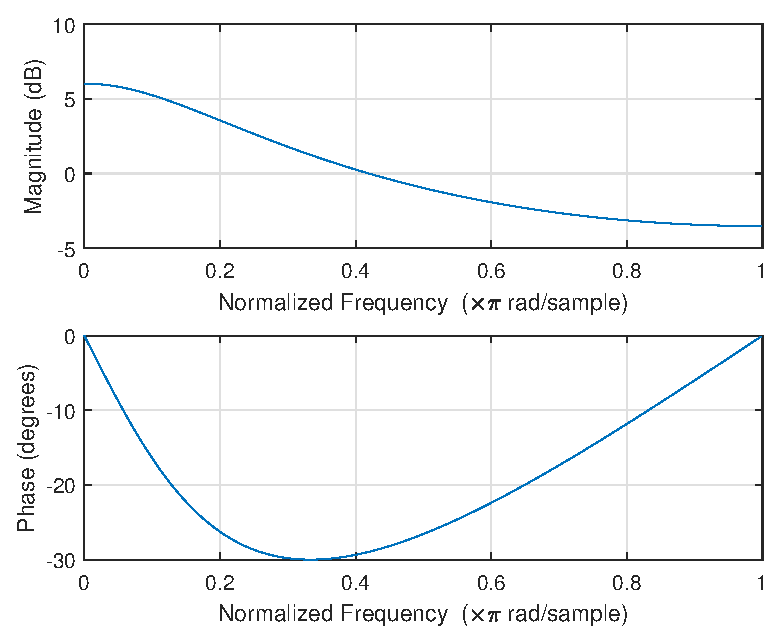
\includegraphics{figs/first_order_sys_freqz.eps}}};
		\node at ($(img1.north east) -(3cm, 0.75cm)$) {$20\log_{10}(|H(e^{j\omega})|)$};
		\node at ($(img1.east)-(3.2cm, 0.5cm)$) {$\angle H(e^{j\omega}) = \arg(H(e^{j\omega}))$};
		\end{tikzpicture}
	\end{center}
\end{frame}

%
\begin{frame}{Phase unwrapping}
	Calculating the phase $\angle H(e^{j\omega})$ using $\arctan(\cdot)$ leads to discontinuities known as \textbf{phase wrapping}, since the image of $\arctan(\cdot)$ is $[-\pi, \pi]$.
	
	\textbf{Phase unwrapping} corrects jumps of $\pm2\pi$ in the phase response.
	
	\begin{center}
		\resizebox{\textwidth}{!}{\begin{tikzpicture}
\begin{axis}[
name=plot1,
axis lines*=middle,
enlargelimits = true, clip=true,
scale only axis,
axis line style={->,>=stealth},
xlabel={$\omega$},
ylabel={$\arg(H(e^{j\omega}))$},
every axis x label/.style={
	at={(ticklabel* cs:1)},
	xshift=-0.2cm,
	anchor=north,
},
every axis y label/.style={
	at={(ticklabel* cs:1)},
	xshift=0.4cm,
	%yshift=0.35cm,
	anchor=south,
},
every outer x axis line/.append style={white!15!black},
every x tick label/.append style={font=\color{white!15!black}},
xmin=0, xmax=3.14,
ymin=-8, ymax=3.14,
xtick={0, 3.14},
xticklabels ={$0$, $\pi$},
ytick={3.14, -3.14, -6.28},
yticklabels={$\pi$, $-\pi$, $-2\pi$},
ymajorgrids,
every outer y axis line/.append style={white!15!black},
every y tick label/.append style={font=\color{white!15!black}},
legend style={draw=white!15!black,fill=white,legend cell align=left}]
\addplot [smooth, dashed, black!10, line width=1.5pt, forget plot, domain=0:3.14, samples=31] {3*x*(x-pi)};
\addplot [smooth, black, line width=1.5pt, forget plot, domain=0:0.379, samples=11] {3*x*(x-pi)};
\addplot [smooth, black, line width=1.5pt, forget plot, domain=0.379:2.76, samples=11] {2*pi + 3*x*(x-pi)};
\addplot [smooth, black, line width=1.5pt, forget plot, domain=2.76:3.14, samples=11] {3*x*(x-pi)};


\node at (axis cs: 1.5, 3.5) {\Large Wrapped phase};
\only<2|handout:1>{\node at (axis cs: 1.5, -8.5) {\large \texttt{>> angle(H)}};}
\end{axis}

\begin{axis}[
name=plot2,
at= (plot1.east), anchor=west,
xshift=1cm,
axis lines*=middle,
enlargelimits = true, clip=true,
scale only axis,
axis line style={->,>=stealth},
xlabel={$\omega$},
ylabel={$\arg(H(e^{j\omega}))$},
every axis x label/.style={
	at={(ticklabel* cs:1)},
	xshift=-0.2cm,
	anchor=north,
},
every axis y label/.style={
	at={(ticklabel* cs:1)},
	xshift=0.4cm,
	%yshift=0.35cm,
	anchor=south,
},
every outer x axis line/.append style={white!15!black},
every x tick label/.append style={font=\color{white!15!black}},
xmin=0, xmax=3.14,
ymin=-8, ymax=3.14,
xtick={0, 3.14},
xticklabels ={$0$, $\pi$},
ytick={3.14, -3.14, -6.28},
yticklabels={$\pi$, $-\pi$, $-2\pi$},
ymajorgrids,
every outer y axis line/.append style={white!15!black},
every y tick label/.append style={font=\color{white!15!black}},
legend style={draw=white!15!black,fill=white,legend cell align=left}]
\addplot [smooth, black, line width=1.5pt, forget plot, domain=0:3.14, samples=31] {3*x*(x-pi)};

\node at (axis cs: 1.5, 3.5) {\Large Unwrapped phase};
\only<2|handout:1>{\node at (axis cs: 1.5, -8.5) {\large \texttt{>> unwrap(angle(H))}};}

\end{axis}

\end{tikzpicture}}
	\end{center}	
	
\end{frame}

%
\begin{frame}{Group delay}
	\begin{block}{Definition}
		\begin{equation*}
			\tau_g(\omega) = \mathrm{grd}~ H(e^{j\omega}) \equiv -\dfrac{d}{d\omega}\mathrm{arg} H(e^{j\omega}) \tag{group delay}
		\end{equation*}
		
		Group delay measures by how much $e^{j\omega}$ is delayed by the LTI system. 
		
		In continuous-time, $\tau_g(\omega)$ has units of seconds. In discrete-time, $\tau_g(\omega)$ has units of samples.
	\end{block}
	
	\begin{block}{Example}
		If a system has linear phase:
		\begin{equation*}
			\mathrm{arg} H(e^{j\omega}) = -\omega n_d \tag{\textbf{linear phase}}
		\end{equation*} 
		
		Then, the group delay is constant:
		\begin{equation*}
		\tau_g(\omega) = -\dfrac{d}{d\omega}(-\omega n_d) = n_d \tag{\textbf{constant group delay}}
		\end{equation*} 
		
		\textbf{Conclusion:} Linear-phase systems delay all frequencies equally.	
	\end{block}
\end{frame}


\begin{frame}{Effect of group delay}
	Consider the \underline{causal} LTI system defined by the following $z$-transform
	\begin{align*}
	&H(z) = \\ &\bigg(\frac{(1-0.98e^{j0.8\pi}z^{-1})(1-0.98e^{-j0.8\pi}z^{-1})}{(1-0.8e^{j0.4\pi}z^{-1})(1-0.8e^{-j0.4\pi}z^{-1})}\bigg)\prod_{k=1}^4\bigg(\frac{(c_k^* -z^{-1})(c_k -z^{-1})}{(1 -c_kz^{-1})(1 -c_k^*z^{-1})}\bigg)^2
	\end{align*}
	where $c_k = 0.95e^{j(0.15\pi + 0.02\pi k)}$
	
	It has the following pole-zero plot:
	
	\begin{center}
		\resizebox{0.5\linewidth}{!}{\begin{tikzpicture}
\begin{axis}[
axis equal,
axis lines*=middle,
enlargelimits = false, clip=true,
xmin=-1.39,
xmax=1.39,
ymin=-1.10,
ymax=1.10,
axis line style={->,>=stealth},
xlabel={$\mathrm{Re}\{z\}$},
ylabel={$\mathrm{Im}\{z\}$},
every axis x label/.style={
at={(ticklabel* cs:1)},
anchor=north,
},
every axis y label/.style={
at={(ticklabel* cs:1)},
anchor=south,
},
xmajorgrids,
ymajorgrids,
every outer y axis line/.append style={white!15!black},
every y tick label/.append style={font=\color{white!15!black}},
legend style={draw=white!15!black,fill=white,legend cell align=left}]
\draw (axis cs:0,0) circle [black!50, dashed, line width=2pt, radius=1];
\addplot [line width=1pt,mark=x, only marks, mark size = 3pt]
table[row sep=crcr]{
	0.24721 0.76085 \\
	0.24721 -0.76085 \\
	0.8177 0.48359 \\
	0.78573 0.53398 \\
	0.75065 0.58226 \\
	0.71261 0.62825 \\
	0.8177 0.48359 \\
	0.78573 0.53398 \\
	0.75065 0.58226 \\
	0.71261 0.62825 \\
	0.8177 -0.48359 \\
	0.78573 -0.53398 \\
	0.75065 -0.58226 \\
	0.71261 -0.62825 \\
	0.8177 -0.48359 \\
	0.78573 -0.53398 \\
	0.75065 -0.58226 \\
	0.71261 -0.62825 \\
};

\addplot [line width=1pt,mark=*, only marks, mark size = 3pt, mark options={fill=white}]
table[row sep=crcr]{
	-0.79284 0.57603 \\
	-0.79284 -0.57603 \\
	0.90604 -0.53583 \\
	0.87061 -0.59167 \\
	0.83174 -0.64517 \\
	0.78959 -0.69612 \\
	0.90604 -0.53583 \\
	0.87061 -0.59167 \\
	0.83174 -0.64517 \\
	0.78959 -0.69612 \\
	0.90604 0.53583 \\
	0.87061 0.59167 \\
	0.83174 0.64517 \\
	0.78959 0.69612 \\
	0.90604 0.53583 \\
	0.87061 0.59167 \\
	0.83174 0.64517 \\
	0.78959 0.69612 \\
};

% Annotations
\node[align=left, anchor=south] at(axis cs: 0.65, -0.67) {\scriptsize $2$};
\node[align=left, anchor=south] at(axis cs: 0.68, -0.61) {\scriptsize $2$};
\node[align=left, anchor=south] at(axis cs: 0.74, -0.56) {\scriptsize $2$};
\node[align=left, anchor=south] at(axis cs: 0.78, -0.5) {\scriptsize $2$};

\node[align=left, anchor=south] at(axis cs: 0.64, 0.5) {\scriptsize $2$};
\node[align=left, anchor=south] at(axis cs: 0.68, 0.45) {\scriptsize $2$};
\node[align=left, anchor=south] at(axis cs: 0.72, 0.40) {\scriptsize $2$};
\node[align=left, anchor=south] at(axis cs: 0.75, 0.34) {\scriptsize $2$};

\node[align=left, anchor=south] at(axis cs: 0.82445, 0.69612) {\scriptsize $2$};
\node[align=left, anchor=south] at(axis cs: 0.8666, 0.64517) {\scriptsize $2$};
\node[align=left, anchor=south] at(axis cs: 0.97, 0.52) {\scriptsize $2$};
\node[align=left, anchor=south] at(axis cs: 0.87, -0.83) {\scriptsize $2$};

\node[align=left, anchor=south] at(axis cs: 0.99, -0.64) {\scriptsize $2$};
\node[align=left, anchor=south] at(axis cs: 0.96, -0.72) {\scriptsize $2$};
\node[align=left, anchor=south] at(axis cs: 0.92, 0.59167) {\scriptsize $2$};
\node[align=left, anchor=south] at(axis cs: 0.92, -0.79) {\scriptsize $2$};
\end{axis}
\end{tikzpicture}}
	\end{center}
\end{frame}

%
\begin{frame}{Effect of group delay}
	\begin{block}{Phase}
		\begin{center}
			\resizebox{0.7\linewidth}{!}{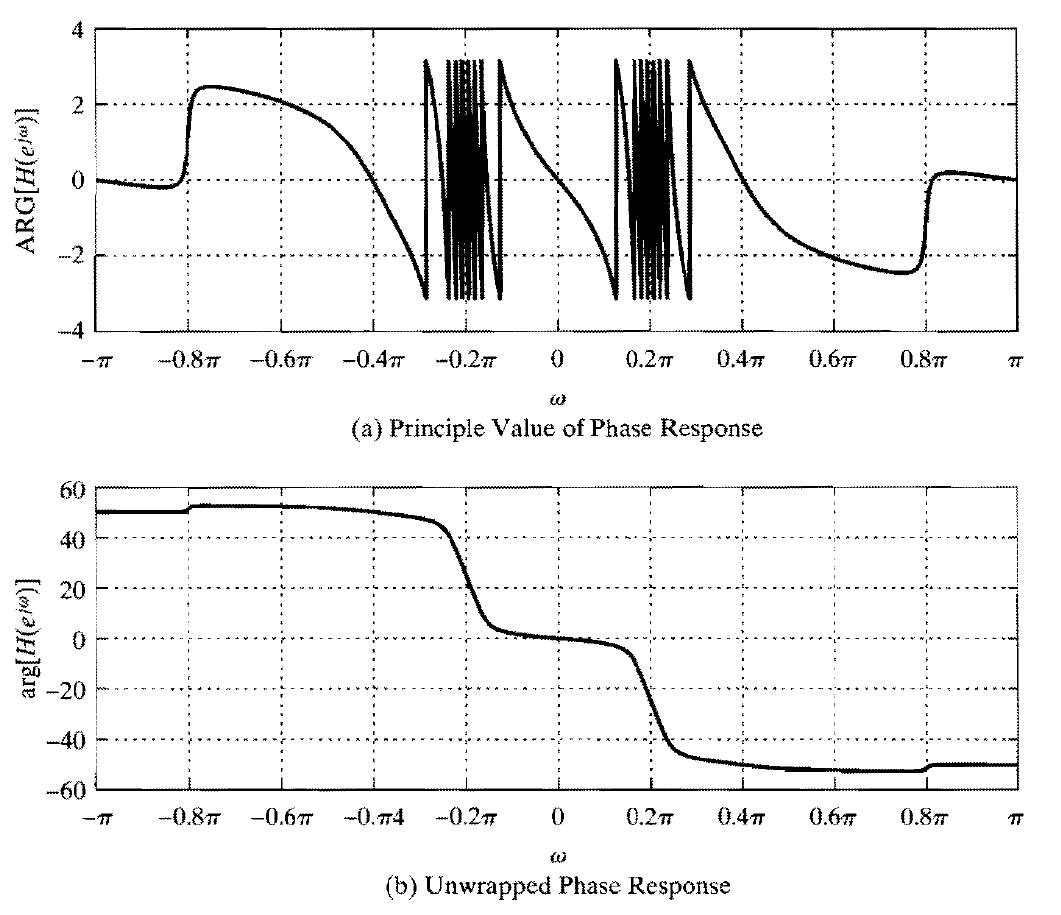
\includegraphics{figs/group_delay_example_phase.png}}
		\end{center}		
	\end{block}
\end{frame}

\begin{frame}{Effect of group delay}
	\begin{block}{Group delay and magnitude}
		\begin{center}
			\resizebox{0.7\linewidth}{!}{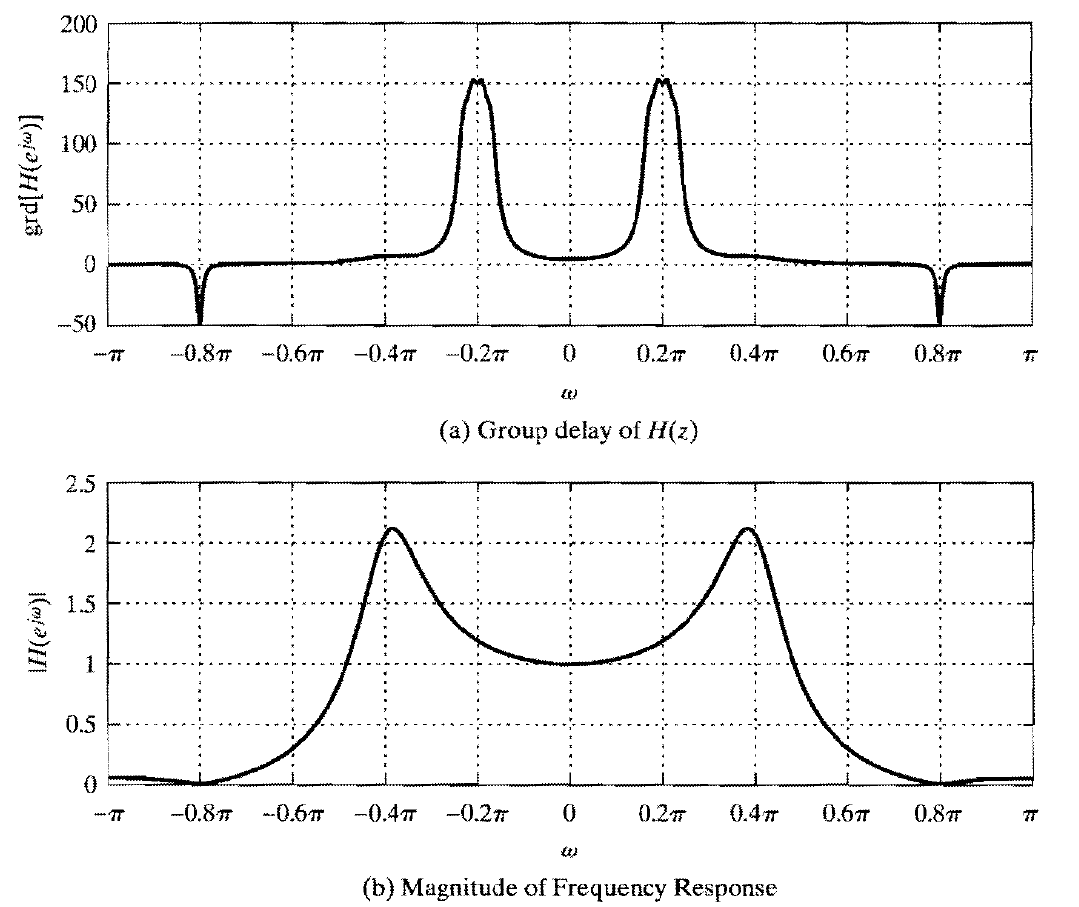
\includegraphics{figs/group_delay_example_delay_magnitude.png}}
		\end{center}		
	\end{block}
\end{frame}

\begin{frame}{Effect of group delay}
	\begin{block}{Consider the following input signal}
		Three sinusoidal pulses of frequencies $\omega_1 = 0.8\pi$, $\omega_2 = 0.2\pi$, and $\omega_3 = 0.4\pi$.
		
	\begin{center}
		\begin{tikzpicture}
		\node (img1) {\resizebox{0.7\linewidth}{!}{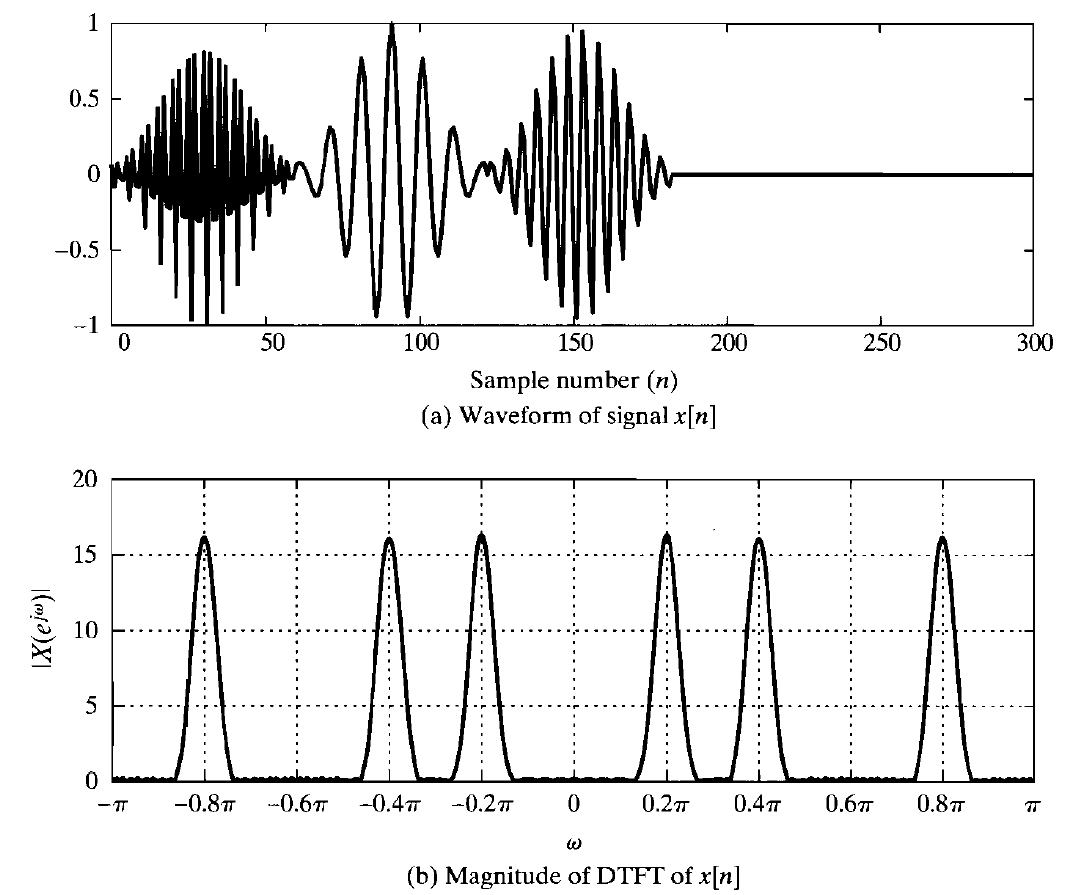
\includegraphics{figs/group_delay_example_input.png}}};
		\node[fill=blue2!20, minimum width=1cm, scale=0.3] (l1) at ($(img1.north west)+(1.5cm, -0cm)$) {\Huge $\omega_1 = 0.8\pi$};
		\node[fill=red2!20, scale=0.3, right=0.25cm of l1] (l2) {\Huge $\omega_2 = 0.2\pi$};
		\node[fill=green2!20, scale=0.3, right=0.25cm of l2] (l3) {\Huge $\omega_3 = 0.4\pi$};
		\node[fill=blue2!20, minimum width=1cm, scale=0.3] (l4) at ($(img1.south east)+(-1.05cm, 2.8cm)$) {\Huge $\omega_1$};
		\node[fill=red2!20, minimum width=1cm, scale=0.3, left=1.6cm of l4] (l5)  {\Huge $\omega_2$};
		\node[fill=green2!20, minimum width=1cm, scale=0.3, left=1cm of l4] (l6)  {\Huge $\omega_3$};
		\end{tikzpicture}
	\end{center}	
	\end{block}
\end{frame}

\begin{frame}{Effect of group delay}
	\begin{block}{Output}
		\vspace{-0.5cm}
		\begin{center}
			\begin{tikzpicture}
			\node (img1) {\resizebox{0.57\linewidth}{!}{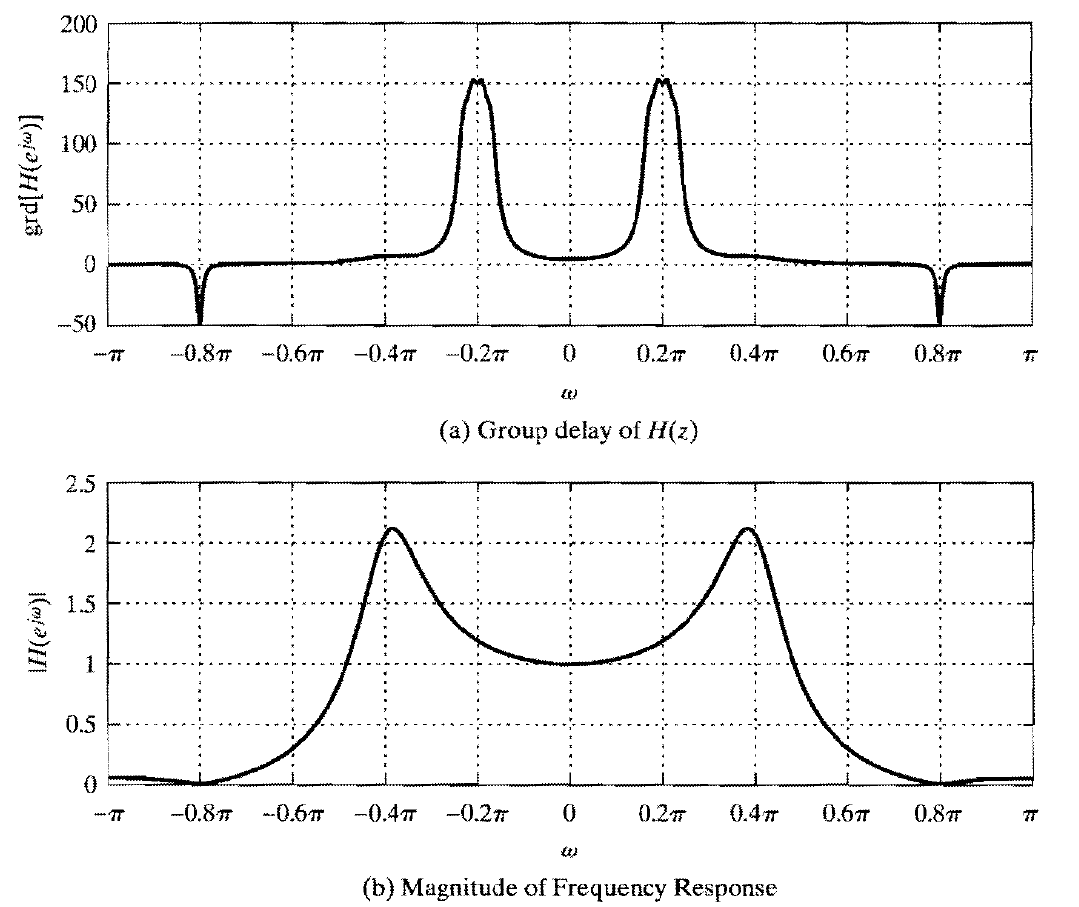
\includegraphics{figs/group_delay_example_delay_magnitude.png}}};
			\node[below=0cm of img1] (img2) {\resizebox{0.55\linewidth}{!}{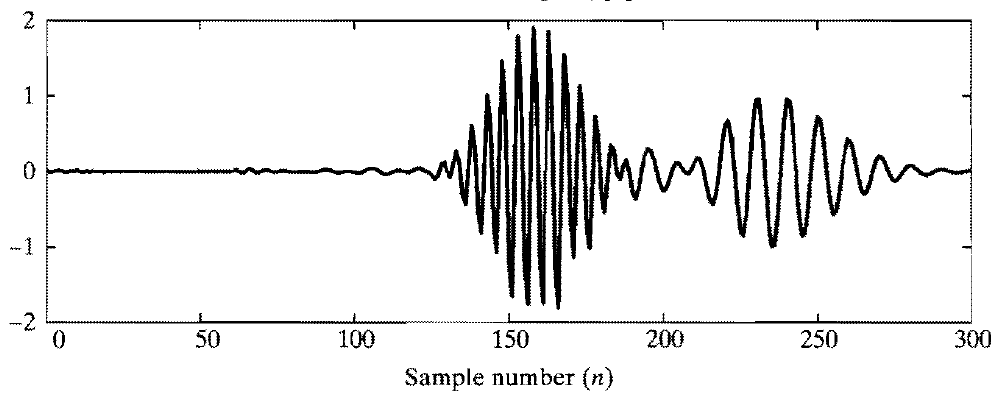
\includegraphics{figs/group_delay_example_output.png}}};

			\node[fill=blue2!20, minimum width=1cm, scale=0.3] (l4) at ($(img1.north east)-(0.9cm, 0.5cm)$) {\Huge $\omega_1$};
			\node[fill=red2!20, minimum width=1cm, scale=0.3, left=1.2cm of l4] (l5)  {\Huge $\omega_2$};
			\node[fill=green2!20, minimum width=1cm, scale=0.3, left=0.7cm of l4] (l6)  {\Huge $\omega_3$};
			
			\node[fill=blue2!20, minimum width=1cm, scale=0.3] (l1) at ($(img1.south east)+(-0.9cm, 2.5cm)$) {\Huge $\omega_1$};
			\node[fill=red2!20, minimum width=1cm, scale=0.3, left=1.2cm of l1] (l2)  {\Huge $\omega_2$};
			\node[fill=green2!20, minimum width=1cm, scale=0.3, left=0.7cm of l1] (l3)  {\Huge $\omega_3$};
			
			\node[fill=blue2!20, minimum width=1cm, scale=0.3] (l7) at ($(img2.north east)+(-5cm, -0.25cm)$) {\Huge $\xcancel{\omega_1 = 0.8\pi}$};
			\node[fill=red2!20, scale=0.3, right=2.5cm of l7] (l9) {\Huge $\omega_2 = 0.2\pi$};
			\node[fill=green2!20, scale=0.3, right=0.9cm of l7] (l8) {\Huge $\omega_3 = 0.4\pi$};
			 
			\end{tikzpicture}
		\end{center}	
	\end{block}
\end{frame}

\begin{frame}<beamer:0|handout:1>

Comments:
\begin{itemize}
	\item The sinusoidal pulse of frequency $\omega_1 = 0.8\pi$ was virtually eliminated, since $H(z)$ has a zero at frequency $0.8\pi$.
	\item The sinusoidal pulse of frequency $\omega_2 = 0.2\pi$ had a gain of about 1.2, but note that the group delay at that frequency is 150 samples.
	\item The sinusoidal pulse of frequency $\omega_3 = 0.4\pi$ had its amplitude doubled, but remained centered around $n = 150$, since the group delay of $H(z)$ around $0.4\pi$ is negligible.
	\item Interestingly, the effect of the system was to switch the position of the two pulses in time. Note that now, the pulse of frequency $\omega_3 = 0.4\pi$ comes before the pulse of frequency $\omega_2 = 0.2\pi$.
\end{itemize}

\end{frame}


%
\section{Poles, Zeros, and the Frequency Response}
\begin{frame}<beamer:1|handout:0>{Outline}
\tableofcontents[currentsection]
\end{frame}

\begin{frame}{Poles and zeros}

The \textbf{zeros} of $H(z)$ are the values of $z$ for which $H(z) = 0$, while the \textbf{poles} of $H(z)$ are the values of $z$ for which $H(z) = \infty$. 

For \textbf{rational $z$-transforms} (ratio of two polynomials in $z^{-1}$ or $z$), zeros and poles are the roots of the numerator and denominator polynomials, respectively.
\begin{align*}
H(z) &= \frac{B(z)}{A(z)} = \frac{b_0 + b_1z^{-1}+\ldots+b_Mz^{-M}}{a_0 + a_1z^{-1}+\ldots+a_Nz^{-N}} \\
&= \frac{b_0}{a_0}z^{N-M}\frac{(z-z_1)(z-z_2)\ldots(z-z_M)}{(z-p_1)(z-p_2)\ldots(z-p_N)}
\end{align*}
\begin{itemize}
	\pause\item If the coefficients $\{b_0, \ldots, b_M\}, \{a_0, \ldots, a_N\}$ are \underline{real}, the poles and zeros are either \underline{real} or they appear in \underline{complex conjugate pairs}
	\pause\item $H(z)$ has \textbf{finite impulse response (FIR)} if $a_k = 0, k = 1, \ldots N$ i.e., all poles of $H(z)$ are at the origin.
	\pause\item $H(z)$ has \textbf{infinite impulse response (IIR)} if $H(z)$ has poles away from the origin.
\end{itemize}	
\end{frame}

%
\begin{frame}{Poles, zeros, and the frequency response}

\textbf{Question:} How do poles and zeros affect the frequency response?

\textbf{Effect of a zero:} $H(z) = 1 - re^{j\theta}z^{-1}$

\begin{columns}[t]
	\begin{column}{0.7\textwidth}
		\vspace{-0.5cm}
		\begin{center}
			\resizebox{\linewidth}{!}{\begin{tikzpicture}
\begin{axis}[
axis equal,
axis lines*=middle,
enlargelimits = false, clip=true,
xmin=-1.39,
xmax=1.39,
ymin=-1.10,
ymax=1.10,
axis line style={->,>=stealth},
xlabel={$\mathrm{Re}\{z\}$},
ylabel={$\mathrm{Im}\{z\}$},
every axis x label/.style={
at={(ticklabel* cs:1)},
anchor=north,
},
every axis y label/.style={
at={(ticklabel* cs:1)},
anchor=south,
},
xtick=1, ytick=\empty,
xticklabel style={xshift=0.1cm},
every outer y axis line/.append style={white!15!black},
every y tick label/.append style={font=\color{white!15!black}},
legend style={draw=white!15!black,fill=white,legend cell align=left}]
\draw (axis cs:0,0) circle [black!50, dashed, line width=2pt, radius=1];
\addplot [line width=1pt,mark=x, only marks, mark size = 3pt]
table[row sep=crcr]{
	0 0 \\
};

\addplot [line width=1pt,mark=*, only marks, mark size = 3pt, mark options={fill=white}]
table[row sep=crcr]{
	0.3 0.8\\
};

\coordinate (axis) at (axis cs: 1, 0);
\coordinate (orig) at (axis cs: 0, 0);
\coordinate (zero) at (axis cs:	0.3, 0.8);
\coordinate (eval) at (axis cs:	0.9397, 0.3420);

\draw[->, >=stealth, shorten >= 2.5pt, thick] (orig) -- (zero);
\pic [draw, <->, "$\theta$", angle eccentricity=1.5] {angle = axis--orig--zero};

\only<2-|handout:1-2>{
\pic [draw, red2, <->, "$\omega$", angle eccentricity=1.25,  angle radius=1cm] {angle = axis--orig--eval};
\draw[->, >=stealth, shorten >= 2.5pt, thick, red2] (orig) -- (eval);
\draw[red2, fill=red2] (eval) circle (3pt);
}

\only<3-|handout:1-2>{
\node at ($(orig)!0.5!(zero) + (-0.1cm, 0.3cm)$) {$v_2$};
\node[red2] at ($(orig)!0.5!(eval) + (0.1cm, 0.3cm)$) {$v_1$};
\draw[->, >=stealth, shorten >= 2.5pt, thick, blue2] (zero) -- (eval);
\node[blue2] at ($(eval)!0.5!(zero) + (-0.1cm, 0.3cm)$) {$v_3$};
}

\end{axis}
\end{tikzpicture}}
		\end{center}
	\end{column}

	\begin{column}{0.3\textwidth}	
		\only<3|handout:1>{
		\textbf{Magnitude}
		\flushleft
		\begin{align*}
		H(z) &= \frac{z - re^{j\theta}}{z} \\
		|H(e^{j\omega})| &= \bigg|\frac{e^{j\omega} - re^{j\theta}}{e^{j\omega}}\bigg| \\
		&= \bigg|\bigg|\frac{{\color{red2} v_1} - {\color{black} v_2}}{{\color{red2} v_1}}\bigg|\bigg|\\
		&= \frac{||{\color{blue2} v_3}||}{||{\color{red2} v_1}||} \\
		&= ||{\color{blue2} v_3}||
		\end{align*}
	}

	\only<4|handout:2>{
	\textbf{Phase}
	\flushleft
	\begin{align*}
	H(z) &= \frac{z - e^{j\theta}}{z} \\
	\angle H(e^{j\omega}) &= \angle \frac{e^{j\omega} - re^{j\theta}}{e^{j\omega}} \\
	&= \angle(e^{j\omega} - re^{j\theta}) \\
	&- \angle e^{j\omega} \\
	&= \angle ({\color{red2} v_1}  - {\color{black} v_2}) - \angle {\color{red2} v_1} \\
	&= \angle {\color{blue2} v_3} - \omega
	\end{align*}
	}
	\end{column}
\end{columns}
\end{frame}

%
\begin{frame}{Poles, zeros, and the frequency response}
	
	\textbf{Effect of a pole:} $H(z) = \displaystyle\frac{1}{1 - re^{j\theta}z^{-1}}$
		
		\begin{columns}[t]
			\begin{column}{0.7\textwidth}
				\vspace{-0.5cm}
				\begin{center}
					\resizebox{\linewidth}{!}{\begin{tikzpicture}
\begin{axis}[
axis equal,
axis lines*=middle,
enlargelimits = false, clip=true,
xmin=-1.39,
xmax=1.39,
ymin=-1.10,
ymax=1.10,
axis line style={->,>=stealth},
xlabel={$\mathrm{Re}\{z\}$},
ylabel={$\mathrm{Im}\{z\}$},
every axis x label/.style={
at={(ticklabel* cs:1)},
anchor=north,
},
every axis y label/.style={
at={(ticklabel* cs:1)},
anchor=south,
},
xtick=1, ytick=\empty,
xticklabel style={xshift=0.1cm},
every outer y axis line/.append style={white!15!black},
every y tick label/.append style={font=\color{white!15!black}},
legend style={draw=white!15!black,fill=white,legend cell align=left}]
\draw (axis cs:0,0) circle [black!50, dashed, line width=2pt, radius=1];
\addplot [line width=1pt,mark=x, only marks, mark size = 3pt]
table[row sep=crcr]{
	0.3 0.8\\
};

\addplot [line width=1pt,mark=*, only marks, mark size = 3pt, mark options={fill=white}]
table[row sep=crcr]{
	0 0 \\
};

\coordinate (axis) at (axis cs: 1, 0);
\coordinate (orig) at (axis cs: 0, 0);
\coordinate (zero) at (axis cs:	0.3, 0.8);
\coordinate (eval) at (axis cs:	0.9397, 0.3420);

\draw[->, >=stealth, shorten >= 2.5pt, thick] (orig) -- (zero);
\pic [draw, <->, "$\theta$", angle eccentricity=1.5] {angle = axis--orig--zero};

\only<2-|handout:1-2>{
\pic [draw, red2, <->, "$\omega$", angle eccentricity=1.25,  angle radius=1cm] {angle = axis--orig--eval};
\draw[->, >=stealth, shorten >= 2.5pt, thick, red2] (orig) -- (eval);
\draw[red2, fill=red2] (eval) circle (3pt);
}

\only<3-|handout:1-2>{
\node at ($(orig)!0.5!(zero) + (-0.1cm, 0.3cm)$) {$v_2$};
\node[red2] at ($(orig)!0.5!(eval) + (0.1cm, 0.3cm)$) {$v_1$};
\draw[->, >=stealth, shorten >= 2.5pt, thick, blue2] (zero) -- (eval);
\node[blue2] at ($(eval)!0.5!(zero) + (-0.1cm, 0.3cm)$) {$v_3$};
}

\end{axis}
\end{tikzpicture}}
				\end{center}
			\end{column}
			
			\begin{column}{0.3\textwidth}	
				\only<3|handout:1>{
					\textbf{Magnitude}
					\flushleft
					\begin{align*}
					H(z) &= \frac{z}{z - re^{j\theta}} \\
					|H(e^{j\omega})| &= \bigg|\frac{e^{j\omega}}{e^{j\omega} - re^{j\theta}}\bigg| \\
					&= \bigg|\frac{{\color{red2} v_1}}{{\color{red2} v_1} - {\color{black} v_2}}\bigg|\\
					&= \frac{||{\color{red2} v_1}||}{||{\color{blue2} v_3}||} \\
					&= \frac{1}{||{\color{blue2} v_3}||}
					\end{align*}
				}
				
				\only<4|handout:2>{
					\textbf{Phase}
					\flushleft
					\begin{align*}
					H(z) &= \frac{z}{z - re^{j\theta}} \\
					\angle H(e^{j\omega}) &= \angle \frac{e^{j\omega}}{e^{j\omega} - re^{j\theta}} \\
					&= -\angle(e^{j\omega} - re^{j\theta}) \\
					&+ \angle e^{j\omega} \\
					&= -\angle {\color{blue2} v_3} + \angle {\color{red2} v_1} \\
					&= -\angle {\color{blue2} v_3} + \omega
					\end{align*}
				}
			\end{column}
		\end{columns}
\end{frame}

%
\begin{frame}{Poles, zeros, and the frequency response}

Summary of effect of poles and zeros

\begin{center}
	\begin{tabular}{c|c|c}
	& Magnitude & Phase \\
	\hline
	Zero & $||{\color{blue2} v_3}||$ & $\angle {\color{blue2} v_3} - \omega$ \\
	Pole & $\displaystyle\frac{1}{||{\color{blue2} v_3}||}$ & $-\angle {\color{blue2} v_3} + \omega$ \\
	\hline
\end{tabular}
\end{center}

\begin{itemize}
	\pause\item As $e^{j\omega}$ approaches a zero, $|H(e^{j\omega})| \to 0$
	\pause\item As $e^{j\omega}$ approaches a zero, $\angle |H(e^{j\omega})|$ decreases ($- \omega$ factor).
	\pause\item At the zero there will be a negative-to-positive sign change of the phase response (\textbf{phase advance}) (must account effect of other zeros/poles)
	\pause\item As $e^{j\omega}$ approaches a pole, $|H(e^{j\omega})| \to \infty$
	\pause\item As $e^{j\omega}$ approaches a pole, $\angle |H(e^{j\omega})|$ increases ($+ \omega$ factor)
	\pause\item At the pole there will be a positive-to-negative sign change of the phase response (\textbf{phase lag}) (must account effect of other zeros/poles).	
\end{itemize}

\pause
\textbf{Conclusion:} Zeros decrease the magnitude and introduce phase advance (negative group delay), while poles increase magnitude and introduce phase lag (positive group delay)

\end{frame}

%
\begin{frame}{Poles, zeros, and the frequency response}
	Example: $H(z) = 1 - 0.9e^{j\pi/4}z^{-1}$
	\begin{center}
		\resizebox{\linewidth}{!}{\begin{tikzpicture}
\begin{axis}[
name=plot1,
axis equal,
axis lines*=middle,
enlargelimits = false, clip=true,
xmin=-1.39,
xmax=1.39,
ymin=-1.10,
ymax=1.10,
axis line style={->,>=stealth},
xlabel={$\mathrm{Re}\{z\}$},
ylabel={$\mathrm{Im}\{z\}$},
every axis x label/.style={
at={(ticklabel* cs:1)},
anchor=north,
},
every axis y label/.style={
at={(ticklabel* cs:1)},
anchor=south,
},
xtick=1, ytick=\empty,
xticklabel style={xshift=0.1cm},
every outer y axis line/.append style={white!15!black},
every y tick label/.append style={font=\color{white!15!black}},
legend style={draw=white!15!black,fill=white,legend cell align=left}]
\draw (axis cs:0,0) circle [black!50, dashed, line width=2pt, radius=1];
\addplot [line width=1pt,mark=x, only marks, mark size = 3pt]
table[row sep=crcr]{
	0 0 \\
};

\addplot [line width=1pt,mark=*, only marks, mark size = 3pt, mark options={fill=white}]
table[row sep=crcr]{
	0.6364 0.6364\\
};

\coordinate (axis) at (axis cs: 1, 0);
\coordinate (orig) at (axis cs: 0, 0);
\coordinate (zero) at (axis cs:	0.6364, 0.6364);
\draw[->, >=stealth, shorten >= 2.5pt, thick] (orig) -- (zero);

\pic [draw, <->, "$\theta$", angle eccentricity=1.5] {angle = axis--orig--zero};

\only<1|handout:0>{
\coordinate (eval) at (axis cs:	1, 0);
%\pic [draw, red2, <->, "$\omega$", angle eccentricity=1.25,  angle radius=1cm] {angle = axis--orig--eval};
\draw[->, >=stealth, shorten >= 2.5pt, thick, red2] (orig) -- (eval);
\draw[red2, fill=red2] (eval) circle (3pt);
\draw[->, >=stealth, shorten >= 2.5pt, thick, blue2] (zero) -- (eval);
}

\only<2|handout:1>{
	\coordinate (eval) at (axis cs:	0.707, 0.707);
	\pic [draw, red2, <->, "$\omega$", angle eccentricity=1.25,  angle radius=1cm] {angle = axis--orig--eval};
	\draw[->, >=stealth, shorten >= 2.5pt, thick, red2] (orig) -- (eval);
	\draw[red2, fill=red2] (eval) circle (3pt);
	\draw[->, >=stealth, shorten >= 2.5pt, thick, blue2] (zero) -- (eval);
}

%\node at ($(orig)!0.5!(zero) + (-0.1cm, 0.3cm)$) {$v_2$};
%\node[red2] at ($(orig)!0.5!(eval) + (0.1cm, 0.3cm)$) {$v_1$};
%\node[blue2] at ($(eval)!0.5!(zero) + (-0.1cm, 0.3cm)$) {$v_3$};

\end{axis}

\begin{axis}[
name=plot2,
at= (plot1.east), anchor=west,
xshift=1cm,
axis lines*=middle,
enlargelimits = upper, clip=true,
scale only axis,
axis line style={->,>=stealth},
xlabel={$\omega$},
ylabel={$20\cdot\log_{10}(|H(e^{j\omega})|)$},
every axis x label/.style={
	at={(ticklabel* cs:1)},
	xshift=-0.2cm,
	anchor=north,
},
every axis y label/.style={
	at={(ticklabel* cs:1)},
	xshift=0.4cm,
	%yshift=0.35cm,
	anchor=south,
},
every outer x axis line/.append style={white!15!black},
every x tick label/.append style={font=\color{white!15!black}},
xmin=0, xmax=3.14,
xtick={0, 0.7850, 1.57, 2.3550, 3.14},
xticklabels ={$0$, $\pi/4$, $\pi/2$, $3\pi/4$, $\pi$},
ymajorgrids,
every outer y axis line/.append style={white!15!black},
every y tick label/.append style={font=\color{white!15!black}},
legend style={draw=white!15!black,fill=white,legend cell align=left}]
\addplot [smooth, black, line width=1.5pt, forget plot, domain=0:3.14, samples=101] {20*log10(sqrt(1+0.81 - 2*0.9*cos(deg(x)-45)))};

\only<1|handout:0>{
\addplot [red2, mark=*, mark size=3pt] coordinates {(0,-2.6986)};
}

\only<2|handout:1>{
	\addplot [red2, mark=*, mark size=3pt] coordinates {(0.7854,-20)};
}

\end{axis}
\end{tikzpicture}}
	\end{center}	
\end{frame}

\begin{frame}{Poles, zeros, and the frequency response}
	Example: $H(z) = 1 - 0.9e^{j\pi/4}z^{-1}$
	\begin{center}
		\resizebox{\linewidth}{!}{\begin{tikzpicture}
\begin{axis}[
name=plot1,
axis equal,
axis lines*=middle,
enlargelimits = false, clip=true,
xmin=-1.39,
xmax=1.39,
ymin=-1.10,
ymax=1.10,
axis line style={->,>=stealth},
xlabel={$\mathrm{Re}\{z\}$},
ylabel={$\mathrm{Im}\{z\}$},
every axis x label/.style={
at={(ticklabel* cs:1)},
anchor=north,
},
every axis y label/.style={
at={(ticklabel* cs:1)},
anchor=south,
},
xtick=1, ytick=\empty,
xticklabel style={xshift=0.1cm},
every outer y axis line/.append style={white!15!black},
every y tick label/.append style={font=\color{white!15!black}},
legend style={draw=white!15!black,fill=white,legend cell align=left}]
\draw (axis cs:0,0) circle [black!50, dashed, line width=2pt, radius=1];
\addplot [line width=1pt,mark=x, only marks, mark size = 3pt]
table[row sep=crcr]{
	0 0 \\
};

\addplot [line width=1pt,mark=*, only marks, mark size = 3pt, mark options={fill=white}]
table[row sep=crcr]{
	0.6364 0.6364\\
};

\coordinate (axis) at (axis cs: 1, 0);
\coordinate (orig) at (axis cs: 0, 0);
\coordinate (zero) at (axis cs:	0.6364, 0.6364);
\draw[->, >=stealth, shorten >= 2.5pt, thick] (orig) -- (zero);

\pic [draw, <->, "$\theta$", angle eccentricity=1.5] {angle = axis--orig--zero};

\only<1|handout:0>{
\coordinate (eval) at (axis cs:	1, 0);
%\pic [draw, red2, <->, "$\omega$", angle eccentricity=1.25,  angle radius=1cm] {angle = axis--orig--eval};
\draw[->, >=stealth, shorten >= 2.5pt, thick, red2] (orig) -- (eval);
\draw[red2, fill=red2] (eval) circle (3pt);
\draw[->, >=stealth, shorten >= 2.5pt, thick, blue2] (zero) -- (eval);
}

\only<2|handout:1>{
	\coordinate (eval) at (axis cs:	0.707, 0.707);
	\pic [draw, red2, <->, "$\omega$", angle eccentricity=1.25,  angle radius=1cm] {angle = axis--orig--eval};
	\draw[->, >=stealth, shorten >= 2.5pt, thick, red2] (orig) -- (eval);
	\draw[red2, fill=red2] (eval) circle (3pt);
	\draw[->, >=stealth, shorten >= 2.5pt, thick, blue2] (zero) -- (eval);
}

%\node at ($(orig)!0.5!(zero) + (-0.1cm, 0.3cm)$) {$v_2$};
%\node[red2] at ($(orig)!0.5!(eval) + (0.1cm, 0.3cm)$) {$v_1$};
%\node[blue2] at ($(eval)!0.5!(zero) + (-0.1cm, 0.3cm)$) {$v_3$};

\end{axis}

\begin{axis}[
name=plot2,
at= (plot1.east), anchor=west,
xshift=1cm,
axis lines*=middle,
enlargelimits = upper, clip=true,
scale only axis,
axis line style={->,>=stealth},
xlabel={$\omega$},
ylabel={$\angle H(e^{j\omega})$},
every axis x label/.style={
	at={(ticklabel* cs:1)},
	xshift=-0.2cm,
	anchor=north,
},
every axis y label/.style={
	at={(ticklabel* cs:1)},
	xshift=0.4cm,
	%yshift=0.35cm,
	anchor=south,
},
every outer x axis line/.append style={white!15!black},
every x tick label/.append style={font=\color{white!15!black}},
xmin=0, xmax=3.14,
xtick={0, 0.7850, 1.57, 2.3550, 3.14},
xticklabels ={$0$, $\pi/4$, $\pi/2$, $3\pi/4$, $\pi$},
ymajorgrids,
every outer y axis line/.append style={white!15!black},
every y tick label/.append style={font=\color{white!15!black}},
legend style={draw=white!15!black,fill=white,legend cell align=left}]
\addplot [smooth, black, line width=1.5pt, forget plot, domain=0:3.14, samples=101]
table[row sep=crcr]{
	0 -60.2586 \\
	0.031733 -60.8336 \\
	0.063467 -61.3812 \\
	0.0952 -61.8979 \\
	0.12693 -62.3792 \\
	0.15867 -62.8199 \\
	0.1904 -63.2139 \\
	0.22213 -63.5535 \\
	0.25387 -63.8295 \\
	0.2856 -64.0303 \\
	0.31733 -64.1415 \\
	0.34907 -64.1449 \\
	0.3808 -64.0171 \\
	0.41253 -63.7275 \\
	0.44427 -63.2356 \\
	0.476 -62.4869 \\
	0.50773 -61.406 \\
	0.53947 -59.8875 \\
	0.5712 -57.7798 \\
	0.60293 -54.8614 \\
	0.63467 -50.8046 \\
	0.6664 -45.1296 \\
	0.69813 -37.1777 \\
	0.72986 -26.2297 \\
	0.7616 -12.0591 \\
	0.79333 4.0828 \\
	0.82506 19.5142 \\
	0.8568 32.1148 \\
	0.88853 41.4852 \\
	0.92026 48.2065 \\
	0.952 53.0011 \\
	0.98373 56.4394 \\
	1.0155 58.9191 \\
	1.0472 60.7096 \\
	1.0789 61.9937 \\
	1.1107 62.8975 \\
	1.1424 63.5099 \\
	1.1741 63.8948 \\
	1.2059 64.0991 \\
	1.2376 64.158 \\
	1.2693 64.0981 \\
	1.3011 63.9401 \\
	1.3328 63.7001 \\
	1.3645 63.3911 \\
	1.3963 63.0232 \\
	1.428 62.605 \\
	1.4597 62.1432 \\
	1.4915 61.6437 \\
	1.5232 61.111 \\
	1.5549 60.5493 \\
	1.5867 59.9618 \\
	1.6184 59.3516 \\
	1.6501 58.7209 \\
	1.6819 58.0721 \\
	1.7136 57.4068 \\
	1.7453 56.7268 \\
	1.7771 56.0333 \\
	1.8088 55.3278 \\
	1.8405 54.6111 \\
	1.8723 53.8844 \\
	1.904 53.1484 \\
	1.9357 52.404 \\
	1.9675 51.6517 \\
	1.9992 50.8923 \\
	2.0309 50.1263 \\
	2.0627 49.3541 \\
	2.0944 48.5762 \\
	2.1261 47.793 \\
	2.1579 47.005 \\
	2.1896 46.2123 \\
	2.2213 45.4154 \\
	2.2531 44.6145 \\
	2.2848 43.81 \\
	2.3165 43.0019 \\
	2.3483 42.1905 \\
	2.38 41.3761 \\
	2.4117 40.5589 \\
	2.4435 39.7389 \\
	2.4752 38.9164 \\
	2.5069 38.0915 \\
	2.5387 37.2643 \\
	2.5704 36.435 \\
	2.6021 35.6037 \\
	2.6339 34.7705 \\
	2.6656 33.9355 \\
	2.6973 33.0989 \\
	2.7291 32.2606 \\
	2.7608 31.4208 \\
	2.7925 30.5796 \\
	2.8243 29.737 \\
	2.856 28.8932 \\
	2.8877 28.0481 \\
	2.9195 27.2019 \\
	2.9512 26.3546 \\
	2.9829 25.5063 \\
	3.0147 24.657 \\
	3.0464 23.8068 \\
	3.0781 22.9557 \\
	3.1099 22.1038 \\
	3.1416 21.2511 \\
};

\only<1|handout:0>{
	\addplot [red2, mark=*, mark size=3pt] coordinates {(0,-60)};
}

\only<2|handout:1>{
	\addplot [red2, mark=*, mark size=3pt] coordinates {(0.777,0)};
}

\end{axis}
\end{tikzpicture}}
	\end{center}	
\end{frame}

\begin{frame}{Poles, zeros, and the frequency response}
	Example: $H(z) = \displaystyle\frac{1}{1 - 0.9e^{j\pi/4}z^{-1}}$
	\begin{center}
		\resizebox{\linewidth}{!}{\begin{tikzpicture}
\begin{axis}[
name=plot1,
axis equal,
axis lines*=middle,
enlargelimits = false, clip=true,
xmin=-1.39,
xmax=1.39,
ymin=-1.10,
ymax=1.10,
axis line style={->,>=stealth},
xlabel={$\mathrm{Re}\{z\}$},
ylabel={$\mathrm{Im}\{z\}$},
every axis x label/.style={
at={(ticklabel* cs:1)},
anchor=north,
},
every axis y label/.style={
at={(ticklabel* cs:1)},
anchor=south,
},
xtick=1, ytick=\empty,
xticklabel style={xshift=0.1cm},
every outer y axis line/.append style={white!15!black},
every y tick label/.append style={font=\color{white!15!black}},
legend style={draw=white!15!black,fill=white,legend cell align=left}]
\draw (axis cs:0,0) circle [black!50, dashed, line width=2pt, radius=1];
\addplot [line width=1pt,mark=x, only marks, mark size = 3pt]
table[row sep=crcr]{
	0.6364 0.6364\\
};

\addplot [line width=1pt,mark=*, only marks, mark size = 3pt, mark options={fill=white}]
table[row sep=crcr]{
	0 0 \\
};

\coordinate (axis) at (axis cs: 1, 0);
\coordinate (orig) at (axis cs: 0, 0);
\coordinate (zero) at (axis cs:	0.6364, 0.6364);
\draw[->, >=stealth, shorten >= 2.5pt, thick] (orig) -- (zero);

\pic [draw, <->, "$\theta$", angle eccentricity=1.5] {angle = axis--orig--zero};

\only<1|handout:0>{
\coordinate (eval) at (axis cs:	1, 0);
%\pic [draw, red2, <->, "$\omega$", angle eccentricity=1.25,  angle radius=1cm] {angle = axis--orig--eval};
\draw[->, >=stealth, shorten >= 2.5pt, thick, red2] (orig) -- (eval);
\draw[red2, fill=red2] (eval) circle (3pt);
\draw[->, >=stealth, shorten >= 2.5pt, thick, blue2] (zero) -- (eval);
}

\only<2|handout:1>{
	\coordinate (eval) at (axis cs:	0.707, 0.707);
	\pic [draw, red2, <->, "$\omega$", angle eccentricity=1.25,  angle radius=1cm] {angle = axis--orig--eval};
	\draw[->, >=stealth, shorten >= 2.5pt, thick, red2] (orig) -- (eval);
	\draw[red2, fill=red2] (eval) circle (3pt);
	\draw[->, >=stealth, shorten >= 2.5pt, thick, blue2] (zero) -- (eval);
}

%\node at ($(orig)!0.5!(zero) + (-0.1cm, 0.3cm)$) {$v_2$};
%\node[red2] at ($(orig)!0.5!(eval) + (0.1cm, 0.3cm)$) {$v_1$};
%\node[blue2] at ($(eval)!0.5!(zero) + (-0.1cm, 0.3cm)$) {$v_3$};

\end{axis}

\begin{axis}[
name=plot2,
at= (plot1.east), anchor=west,
xshift=1cm,
axis lines*=middle,
enlargelimits = upper, clip=true,
scale only axis,
axis line style={->,>=stealth},
xlabel={$\omega$},
ylabel={$20\cdot\log_{10}(|H(e^{j\omega})|)$},
every axis x label/.style={
	at={(ticklabel* cs:1)},
	xshift=-0.2cm,
	anchor=north,
},
every axis y label/.style={
	at={(ticklabel* cs:1)},
	xshift=0.4cm,
	%yshift=0.35cm,
	anchor=south,
},
every outer x axis line/.append style={white!15!black},
every x tick label/.append style={font=\color{white!15!black}},
xmin=0, xmax=3.14,
xtick={0, 0.7850, 1.57, 2.3550, 3.14},
xticklabels ={$0$, $\pi/4$, $\pi/2$, $3\pi/4$, $\pi$},
ymajorgrids,
every outer y axis line/.append style={white!15!black},
every y tick label/.append style={font=\color{white!15!black}},
legend style={draw=white!15!black,fill=white,legend cell align=left}]
\addplot [smooth, black, line width=1.5pt, forget plot, domain=0:3.14, samples=101] {-20*log10(sqrt(1+0.81 - 2*0.9*cos(deg(x)-45)))};

\only<1|handout:0>{
\addplot [red2, mark=*, mark size=3pt] coordinates {(0,2.6986)};
}

\only<2|handout:1>{
	\addplot [red2, mark=*, mark size=3pt] coordinates {(0.7854, 20)};
}

\end{axis}
\end{tikzpicture}}
	\end{center}	
\end{frame}

\begin{frame}{Poles, zeros, and the frequency response}
	Example: $H(z) = \displaystyle\frac{1}{1 - 0.9e^{j\pi/4}z^{-1}}$
	\begin{center}
		\resizebox{\linewidth}{!}{\begin{tikzpicture}
\begin{axis}[
name=plot1,
axis equal,
axis lines*=middle,
enlargelimits = false, clip=true,
xmin=-1.39,
xmax=1.39,
ymin=-1.10,
ymax=1.10,
axis line style={->,>=stealth},
xlabel={$\mathrm{Re}\{z\}$},
ylabel={$\mathrm{Im}\{z\}$},
every axis x label/.style={
at={(ticklabel* cs:1)},
anchor=north,
},
every axis y label/.style={
at={(ticklabel* cs:1)},
anchor=south,
},
xtick=1, ytick=\empty,
xticklabel style={xshift=0.1cm},
every outer y axis line/.append style={white!15!black},
every y tick label/.append style={font=\color{white!15!black}},
legend style={draw=white!15!black,fill=white,legend cell align=left}]
\draw (axis cs:0,0) circle [black!50, dashed, line width=2pt, radius=1];
\addplot [line width=1pt,mark=x, only marks, mark size = 3pt]
table[row sep=crcr]{
	0.6364 0.6364\\
};

\addplot [line width=1pt,mark=*, only marks, mark size = 3pt, mark options={fill=white}]
table[row sep=crcr]{
	0 0 \\
};

\coordinate (axis) at (axis cs: 1, 0);
\coordinate (orig) at (axis cs: 0, 0);
\coordinate (zero) at (axis cs:	0.6364, 0.6364);
\draw[->, >=stealth, shorten >= 2.5pt, thick] (orig) -- (zero);

\pic [draw, <->, "$\theta$", angle eccentricity=1.5] {angle = axis--orig--zero};

\only<1|handout:0>{
\coordinate (eval) at (axis cs:	1, 0);
%\pic [draw, red2, <->, "$\omega$", angle eccentricity=1.25,  angle radius=1cm] {angle = axis--orig--eval};
\draw[->, >=stealth, shorten >= 2.5pt, thick, red2] (orig) -- (eval);
\draw[red2, fill=red2] (eval) circle (3pt);
\draw[->, >=stealth, shorten >= 2.5pt, thick, blue2] (zero) -- (eval);
}

\only<2|handout:1>{
	\coordinate (eval) at (axis cs:	0.707, 0.707);
	\pic [draw, red2, <->, "$\omega$", angle eccentricity=1.25,  angle radius=1cm] {angle = axis--orig--eval};
	\draw[->, >=stealth, shorten >= 2.5pt, thick, red2] (orig) -- (eval);
	\draw[red2, fill=red2] (eval) circle (3pt);
	\draw[->, >=stealth, shorten >= 2.5pt, thick, blue2] (zero) -- (eval);
}

%\node at ($(orig)!0.5!(zero) + (-0.1cm, 0.3cm)$) {$v_2$};
%\node[red2] at ($(orig)!0.5!(eval) + (0.1cm, 0.3cm)$) {$v_1$};
%\node[blue2] at ($(eval)!0.5!(zero) + (-0.1cm, 0.3cm)$) {$v_3$};

\end{axis}

\begin{axis}[
name=plot2,
at= (plot1.east), anchor=west,
xshift=1cm,
axis lines*=middle,
enlargelimits = upper, clip=true,
scale only axis,
axis line style={->,>=stealth},
xlabel={$\omega$},
ylabel={$\angle H(e^{j\omega})$},
every axis x label/.style={
	at={(ticklabel* cs:1)},
	xshift=-0.2cm,
	anchor=north,
},
every axis y label/.style={
	at={(ticklabel* cs:1)},
	xshift=0.4cm,
	%yshift=0.35cm,
	anchor=south,
},
every outer x axis line/.append style={white!15!black},
every x tick label/.append style={font=\color{white!15!black}},
xmin=0, xmax=3.14,
xtick={0, 0.7850, 1.57, 2.3550, 3.14},
xticklabels ={$0$, $\pi/4$, $\pi/2$, $3\pi/4$, $\pi$},
ymajorgrids,
every outer y axis line/.append style={white!15!black},
every y tick label/.append style={font=\color{white!15!black}},
legend style={draw=white!15!black,fill=white,legend cell align=left}]
\addplot [smooth, black, line width=1.5pt, forget plot, domain=0:3.14, samples=101] 
table[row sep=crcr]{
	0 60.2586 \\
	0.031733 60.8336 \\
	0.063467 61.3812 \\
	0.0952 61.8979 \\
	0.12693 62.3792 \\
	0.15867 62.8199 \\
	0.1904 63.2139 \\
	0.22213 63.5535 \\
	0.25387 63.8295 \\
	0.2856 64.0303 \\
	0.31733 64.1415 \\
	0.34907 64.1449 \\
	0.3808 64.0171 \\
	0.41253 63.7275 \\
	0.44427 63.2356 \\
	0.476 62.4869 \\
	0.50773 61.406 \\
	0.53947 59.8875 \\
	0.5712 57.7798 \\
	0.60293 54.8614 \\
	0.63467 50.8046 \\
	0.6664 45.1296 \\
	0.69813 37.1777 \\
	0.72986 26.2297 \\
	0.7616 12.0591 \\
	0.79333 -4.0828 \\
	0.82506 -19.5142 \\
	0.8568 -32.1148 \\
	0.88853 -41.4852 \\
	0.92026 -48.2065 \\
	0.952 -53.0011 \\
	0.98373 -56.4394 \\
	1.0155 -58.9191 \\
	1.0472 -60.7096 \\
	1.0789 -61.9937 \\
	1.1107 -62.8975 \\
	1.1424 -63.5099 \\
	1.1741 -63.8948 \\
	1.2059 -64.0991 \\
	1.2376 -64.158 \\
	1.2693 -64.0981 \\
	1.3011 -63.9401 \\
	1.3328 -63.7001 \\
	1.3645 -63.3911 \\
	1.3963 -63.0232 \\
	1.428 -62.605 \\
	1.4597 -62.1432 \\
	1.4915 -61.6437 \\
	1.5232 -61.111 \\
	1.5549 -60.5493 \\
	1.5867 -59.9618 \\
	1.6184 -59.3516 \\
	1.6501 -58.7209 \\
	1.6819 -58.0721 \\
	1.7136 -57.4068 \\
	1.7453 -56.7268 \\
	1.7771 -56.0333 \\
	1.8088 -55.3278 \\
	1.8405 -54.6111 \\
	1.8723 -53.8844 \\
	1.904 -53.1484 \\
	1.9357 -52.404 \\
	1.9675 -51.6517 \\
	1.9992 -50.8923 \\
	2.0309 -50.1263 \\
	2.0627 -49.3541 \\
	2.0944 -48.5762 \\
	2.1261 -47.793 \\
	2.1579 -47.005 \\
	2.1896 -46.2123 \\
	2.2213 -45.4154 \\
	2.2531 -44.6145 \\
	2.2848 -43.81 \\
	2.3165 -43.0019 \\
	2.3483 -42.1905 \\
	2.38 -41.3761 \\
	2.4117 -40.5589 \\
	2.4435 -39.7389 \\
	2.4752 -38.9164 \\
	2.5069 -38.0915 \\
	2.5387 -37.2643 \\
	2.5704 -36.435 \\
	2.6021 -35.6037 \\
	2.6339 -34.7705 \\
	2.6656 -33.9355 \\
	2.6973 -33.0989 \\
	2.7291 -32.2606 \\
	2.7608 -31.4208 \\
	2.7925 -30.5796 \\
	2.8243 -29.737 \\
	2.856 -28.8932 \\
	2.8877 -28.0481 \\
	2.9195 -27.2019 \\
	2.9512 -26.3546 \\
	2.9829 -25.5063 \\
	3.0147 -24.657 \\
	3.0464 -23.8068 \\
	3.0781 -22.9557 \\
	3.1099 -22.1038 \\
	3.1416 -21.2511 \\
};

\only<1|handout:0>{
	\addplot [red2, mark=*, mark size=3pt] coordinates {(0,60)};
}

\only<2|handout:1>{
	\addplot [red2, mark=*, mark size=3pt] coordinates {(0.777,0)};
}


\end{axis}
\end{tikzpicture}}
	\end{center}	
\end{frame}

%
\begin{frame}{Match the pole-zero plots to the magnitude responses}
	\hspace*{-1cm}\resizebox{\paperwidth}{!}{\begin{tikzpicture}
\begin{axis}[
name=plot1,
axis equal,
axis lines*=middle,
enlargelimits = false, clip=true,
xmin=-1.39,
xmax=1.39,
ymin=-1.10,
ymax=1.10,
axis line style={->,>=stealth},
xlabel={$\mathrm{Re}\{z\}$},
ylabel={$\mathrm{Im}\{z\}$},
every axis x label/.style={
at={(ticklabel* cs:1)},
anchor=north,
},
every axis y label/.style={
at={(ticklabel* cs:1)},
anchor=south,
},
xtick=1, ytick=\empty,
xticklabel style={xshift=0.1cm},
every outer y axis line/.append style={white!15!black},
every y tick label/.append style={font=\color{white!15!black}},
legend style={draw=white!15!black,fill=white,legend cell align=left}]
\draw (axis cs:0,0) circle [black!50, dashed, line width=2pt, radius=1];
\addplot [line width=1pt,mark=x, only marks, mark size = 3pt]
table[row sep=crcr]{
	0 1e-50 \\
	0 1e-50 \\
	0 1e-50 \\
};

\addplot [line width=1pt,mark=*, only marks, mark size = 3pt, mark options={fill=white}]
table[row sep=crcr]{
	-1 0 \\
	-7.7716e-16 1 \\
	-7.7716e-16 -1 \\
};

% Annotations
\node[align=left, anchor=south] at(axis cs: 0.06, 1e-50) {\large $3$};
\end{axis}


\begin{axis}[
name=plot2,
at= (plot1.east), anchor=west, xshift=1cm,
%at=(plot1.below south east), anchor=above north east,
axis equal,
axis lines*=middle,
enlargelimits = false, clip=true,
xmin=-1.39,
xmax=1.39,
ymin=-1.10,
ymax=1.10,
axis line style={->,>=stealth},
xlabel={$\mathrm{Re}\{z\}$},
ylabel={$\mathrm{Im}\{z\}$},
every axis x label/.style={
	at={(ticklabel* cs:1)},
	anchor=north,
},
every axis y label/.style={
	at={(ticklabel* cs:1)},
	anchor=south,
},
xtick=1, ytick=\empty,
xticklabel style={xshift=0.1cm},
every outer y axis line/.append style={white!15!black},
every y tick label/.append style={font=\color{white!15!black}},
legend style={draw=white!15!black,fill=white,legend cell align=left}]
\draw (axis cs:0,0) circle [black!50, dashed, line width=2pt, radius=1];
\addplot [line width=1pt,mark=x, only marks, mark size = 3pt]
table[row sep=crcr]{
	0.72305 0.5224 \\
	0.72305 -0.5224 \\
	0.683 0 \\
};

\addplot [line width=1pt,mark=*, only marks, mark size = 3pt, mark options={fill=white}]
table[row sep=crcr]{
	0.5083 0.86118 \\
	0.5083 -0.86118 \\
	-1 0 \\
};
\end{axis}

\begin{axis}[
name=plot3,
at= (plot2.east), anchor=west, xshift=1cm,
%at=(plot2.below south east), anchor=above north east,
axis equal,
axis lines*=middle,
enlargelimits = false, clip=true,
xmin=-1.39,
xmax=1.39,
ymin=-1.10,
ymax=1.10,
axis line style={->,>=stealth},
xlabel={$\mathrm{Re}\{z\}$},
ylabel={$\mathrm{Im}\{z\}$},
every axis x label/.style={
	at={(ticklabel* cs:1)},
	anchor=north,
},
every axis y label/.style={
	at={(ticklabel* cs:1)},
	anchor=south,
},
xtick=1, ytick=\empty,
xticklabel style={xshift=0.1cm},
every outer y axis line/.append style={white!15!black},
every y tick label/.append style={font=\color{white!15!black}},
legend style={draw=white!15!black,fill=white,legend cell align=left}]
\draw (axis cs:0,0) circle [black!50, dashed, line width=2pt, radius=1];
\addplot [line width=1pt,mark=x, only marks, mark size = 3pt]
table[row sep=crcr]{
	0.35355 0.35355 \\
	0.35355 -0.35355 \\
};

\addplot [line width=1pt,mark=*, only marks, mark size = 3pt, mark options={fill=white}]
table[row sep=crcr]{
	5.5109e-17 0.9 \\
	5.5109e-17 -0.9 \\
};
\end{axis}

\begin{axis}[
name=plot1a,
at=(plot1.below south east), anchor=above north east,
axis lines*=middle,
enlargelimits = upper, clip=true,
scale only axis,
axis line style={->,>=stealth},
width=0.6\textwidth,
height=0.4\textwidth,
xlabel={$\omega$},
ylabel={$20\cdot\log_{10}(|H(e^{j\omega})|)$},
every axis x label/.style={
	at={(ticklabel* cs:1)},
	xshift=-0.2cm,
	anchor=north,
},
every axis y label/.style={
	at={(ticklabel* cs:1)},
	xshift=0.4cm,
	%yshift=0.35cm,
	anchor=south,
},
every outer x axis line/.append style={white!15!black},
every x tick label/.append style={font=\color{white!15!black}},
xmin=0, xmax=1,
xtick={0, 0.25, 0.5, 0.75, 1},
xticklabels ={$0$, $\pi/4$, $\pi/2$, $3\pi/4$, $\pi$},
ymajorgrids,
every outer y axis line/.append style={white!15!black},
every y tick label/.append style={font=\color{white!15!black}},
legend style={draw=white!15!black,fill=white,legend cell align=left}]
\addplot [color=black, solid, line width=1.5pt, forget plot]
table[row sep=crcr]{
	0 0 \\
	0.0019531 -0.00020439 \\
	0.0039063 -0.00081757 \\
	0.0058594 -0.0018396 \\
	0.0078125 -0.0032705 \\
	0.0097656 -0.0051104 \\
	0.011719 -0.0073594 \\
	0.013672 -0.010018 \\
	0.015625 -0.013085 \\
	0.017578 -0.016563 \\
	0.019531 -0.02045 \\
	0.021484 -0.024747 \\
	0.023438 -0.029454 \\
	0.025391 -0.034573 \\
	0.027344 -0.040102 \\
	0.029297 -0.046042 \\
	0.03125 -0.052395 \\
	0.033203 -0.059159 \\
	0.035156 -0.066336 \\
	0.037109 -0.073926 \\
	0.039062 -0.08193 \\
	0.041016 -0.090348 \\
	0.042969 -0.09918 \\
	0.044922 -0.10843 \\
	0.046875 -0.11809 \\
	0.048828 -0.12817 \\
	0.050781 -0.13867 \\
	0.052734 -0.14958 \\
	0.054688 -0.16091 \\
	0.056641 -0.17267 \\
	0.058594 -0.18484 \\
	0.060547 -0.19743 \\
	0.0625 -0.21045 \\
	0.064453 -0.22388 \\
	0.066406 -0.23775 \\
	0.068359 -0.25203 \\
	0.070312 -0.26674 \\
	0.072266 -0.28188 \\
	0.074219 -0.29744 \\
	0.076172 -0.31343 \\
	0.078125 -0.32985 \\
	0.080078 -0.34671 \\
	0.082031 -0.36399 \\
	0.083984 -0.38171 \\
	0.085938 -0.39986 \\
	0.087891 -0.41844 \\
	0.089844 -0.43747 \\
	0.091797 -0.45693 \\
	0.09375 -0.47683 \\
	0.095703 -0.49717 \\
	0.097656 -0.51795 \\
	0.099609 -0.53918 \\
	0.10156 -0.56085 \\
	0.10352 -0.58297 \\
	0.10547 -0.60553 \\
	0.10742 -0.62855 \\
	0.10938 -0.65201 \\
	0.11133 -0.67593 \\
	0.11328 -0.70031 \\
	0.11523 -0.72514 \\
	0.11719 -0.75043 \\
	0.11914 -0.77618 \\
	0.12109 -0.80239 \\
	0.12305 -0.82907 \\
	0.125 -0.85621 \\
	0.12695 -0.88383 \\
	0.12891 -0.91191 \\
	0.13086 -0.94046 \\
	0.13281 -0.96949 \\
	0.13477 -0.99899 \\
	0.13672 -1.029 \\
	0.13867 -1.0594 \\
	0.14062 -1.0904 \\
	0.14258 -1.1218 \\
	0.14453 -1.1537 \\
	0.14648 -1.1862 \\
	0.14844 -1.2191 \\
	0.15039 -1.2525 \\
	0.15234 -1.2864 \\
	0.1543 -1.3208 \\
	0.15625 -1.3557 \\
	0.1582 -1.3911 \\
	0.16016 -1.427 \\
	0.16211 -1.4635 \\
	0.16406 -1.5004 \\
	0.16602 -1.5379 \\
	0.16797 -1.5759 \\
	0.16992 -1.6144 \\
	0.17188 -1.6535 \\
	0.17383 -1.6931 \\
	0.17578 -1.7332 \\
	0.17773 -1.7738 \\
	0.17969 -1.8151 \\
	0.18164 -1.8568 \\
	0.18359 -1.8991 \\
	0.18555 -1.942 \\
	0.1875 -1.9854 \\
	0.18945 -2.0294 \\
	0.19141 -2.0739 \\
	0.19336 -2.119 \\
	0.19531 -2.1647 \\
	0.19727 -2.211 \\
	0.19922 -2.2578 \\
	0.20117 -2.3053 \\
	0.20312 -2.3533 \\
	0.20508 -2.4019 \\
	0.20703 -2.4511 \\
	0.20898 -2.501 \\
	0.21094 -2.5514 \\
	0.21289 -2.6025 \\
	0.21484 -2.6542 \\
	0.2168 -2.7065 \\
	0.21875 -2.7595 \\
	0.2207 -2.8131 \\
	0.22266 -2.8673 \\
	0.22461 -2.9222 \\
	0.22656 -2.9778 \\
	0.22852 -3.034 \\
	0.23047 -3.0908 \\
	0.23242 -3.1484 \\
	0.23437 -3.2066 \\
	0.23633 -3.2656 \\
	0.23828 -3.3252 \\
	0.24023 -3.3855 \\
	0.24219 -3.4466 \\
	0.24414 -3.5083 \\
	0.24609 -3.5708 \\
	0.24805 -3.634 \\
	0.25 -3.698 \\
	0.25195 -3.7627 \\
	0.25391 -3.8282 \\
	0.25586 -3.8944 \\
	0.25781 -3.9614 \\
	0.25977 -4.0292 \\
	0.26172 -4.0978 \\
	0.26367 -4.1672 \\
	0.26563 -4.2374 \\
	0.26758 -4.3084 \\
	0.26953 -4.3803 \\
	0.27148 -4.453 \\
	0.27344 -4.5266 \\
	0.27539 -4.601 \\
	0.27734 -4.6763 \\
	0.2793 -4.7525 \\
	0.28125 -4.8296 \\
	0.2832 -4.9076 \\
	0.28516 -4.9865 \\
	0.28711 -5.0664 \\
	0.28906 -5.1472 \\
	0.29102 -5.229 \\
	0.29297 -5.3117 \\
	0.29492 -5.3955 \\
	0.29688 -5.4802 \\
	0.29883 -5.566 \\
	0.30078 -5.6529 \\
	0.30273 -5.7408 \\
	0.30469 -5.8297 \\
	0.30664 -5.9198 \\
	0.30859 -6.0109 \\
	0.31055 -6.1032 \\
	0.3125 -6.1966 \\
	0.31445 -6.2912 \\
	0.31641 -6.387 \\
	0.31836 -6.484 \\
	0.32031 -6.5822 \\
	0.32227 -6.6816 \\
	0.32422 -6.7824 \\
	0.32617 -6.8844 \\
	0.32813 -6.9877 \\
	0.33008 -7.0924 \\
	0.33203 -7.1985 \\
	0.33398 -7.306 \\
	0.33594 -7.4149 \\
	0.33789 -7.5252 \\
	0.33984 -7.637 \\
	0.3418 -7.7504 \\
	0.34375 -7.8653 \\
	0.3457 -7.9817 \\
	0.34766 -8.0998 \\
	0.34961 -8.2196 \\
	0.35156 -8.341 \\
	0.35352 -8.4642 \\
	0.35547 -8.5892 \\
	0.35742 -8.7159 \\
	0.35938 -8.8445 \\
	0.36133 -8.975 \\
	0.36328 -9.1075 \\
	0.36523 -9.242 \\
	0.36719 -9.3785 \\
	0.36914 -9.5171 \\
	0.37109 -9.6579 \\
	0.37305 -9.801 \\
	0.375 -9.9463 \\
	0.37695 -10.0939 \\
	0.37891 -10.244 \\
	0.38086 -10.3966 \\
	0.38281 -10.5517 \\
	0.38477 -10.7095 \\
	0.38672 -10.87 \\
	0.38867 -11.0334 \\
	0.39063 -11.1996 \\
	0.39258 -11.3688 \\
	0.39453 -11.5412 \\
	0.39648 -11.7167 \\
	0.39844 -11.8956 \\
	0.40039 -12.0779 \\
	0.40234 -12.2639 \\
	0.4043 -12.4535 \\
	0.40625 -12.647 \\
	0.4082 -12.8444 \\
	0.41016 -13.0461 \\
	0.41211 -13.2521 \\
	0.41406 -13.4626 \\
	0.41602 -13.6779 \\
	0.41797 -13.8981 \\
	0.41992 -14.1235 \\
	0.42188 -14.3542 \\
	0.42383 -14.5907 \\
	0.42578 -14.8331 \\
	0.42773 -15.0818 \\
	0.42969 -15.337 \\
	0.43164 -15.5992 \\
	0.43359 -15.8687 \\
	0.43555 -16.146 \\
	0.4375 -16.4316 \\
	0.43945 -16.7258 \\
	0.44141 -17.0294 \\
	0.44336 -17.3428 \\
	0.44531 -17.6669 \\
	0.44727 -18.0023 \\
	0.44922 -18.3498 \\
	0.45117 -18.7105 \\
	0.45312 -19.0853 \\
	0.45508 -19.4754 \\
	0.45703 -19.8823 \\
	0.45898 -20.3074 \\
	0.46094 -20.7524 \\
	0.46289 -21.2194 \\
	0.46484 -21.7108 \\
	0.4668 -22.2293 \\
	0.46875 -22.7782 \\
	0.4707 -23.3613 \\
	0.47266 -23.9833 \\
	0.47461 -24.6501 \\
	0.47656 -25.3686 \\
	0.47852 -26.148 \\
	0.48047 -26.9997 \\
	0.48242 -27.9389 \\
	0.48438 -28.9864 \\
	0.48633 -30.1708 \\
	0.48828 -31.5347 \\
	0.49023 -33.1434 \\
	0.49219 -35.1071 \\
	0.49414 -37.6316 \\
	0.49609 -41.1793 \\
	0.49805 -47.2262 \\
	0.5 -Inf \\
	0.50195 -47.2795 \\
	0.50391 -41.2859 \\
	0.50586 -37.7915 \\
	0.50781 -35.3203 \\
	0.50977 -33.41 \\
	0.51172 -31.8545 \\
	0.51367 -30.544 \\
	0.51563 -29.4129 \\
	0.51758 -28.4188 \\
	0.51953 -27.533 \\
	0.52148 -26.7347 \\
	0.52344 -26.0088 \\
	0.52539 -25.3437 \\
	0.52734 -24.7304 \\
	0.5293 -24.1618 \\
	0.53125 -23.6323 \\
	0.5332 -23.137 \\
	0.53516 -22.6721 \\
	0.53711 -22.2344 \\
	0.53906 -21.821 \\
	0.54102 -21.4297 \\
	0.54297 -21.0584 \\
	0.54492 -20.7053 \\
	0.54688 -20.369 \\
	0.54883 -20.0481 \\
	0.55078 -19.7414 \\
	0.55273 -19.4479 \\
	0.55469 -19.1666 \\
	0.55664 -18.8967 \\
	0.55859 -18.6374 \\
	0.56055 -18.3881 \\
	0.5625 -18.1481 \\
	0.56445 -17.917 \\
	0.56641 -17.6941 \\
	0.56836 -17.4791 \\
	0.57031 -17.2715 \\
	0.57227 -17.0709 \\
	0.57422 -16.8769 \\
	0.57617 -16.6894 \\
	0.57813 -16.5078 \\
	0.58008 -16.332 \\
	0.58203 -16.1617 \\
	0.58398 -15.9967 \\
	0.58594 -15.8367 \\
	0.58789 -15.6815 \\
	0.58984 -15.5309 \\
	0.5918 -15.3848 \\
	0.59375 -15.243 \\
	0.5957 -15.1052 \\
	0.59766 -14.9715 \\
	0.59961 -14.8415 \\
	0.60156 -14.7153 \\
	0.60352 -14.5926 \\
	0.60547 -14.4733 \\
	0.60742 -14.3574 \\
	0.60937 -14.2447 \\
	0.61133 -14.1351 \\
	0.61328 -14.0286 \\
	0.61523 -13.925 \\
	0.61719 -13.8243 \\
	0.61914 -13.7263 \\
	0.62109 -13.6311 \\
	0.62305 -13.5385 \\
	0.625 -13.4484 \\
	0.62695 -13.3609 \\
	0.62891 -13.2758 \\
	0.63086 -13.193 \\
	0.63281 -13.1126 \\
	0.63477 -13.0345 \\
	0.63672 -12.9585 \\
	0.63867 -12.8848 \\
	0.64063 -12.8131 \\
	0.64258 -12.7435 \\
	0.64453 -12.676 \\
	0.64648 -12.6105 \\
	0.64844 -12.5469 \\
	0.65039 -12.4852 \\
	0.65234 -12.4254 \\
	0.6543 -12.3674 \\
	0.65625 -12.3113 \\
	0.6582 -12.2569 \\
	0.66016 -12.2043 \\
	0.66211 -12.1534 \\
	0.66406 -12.1042 \\
	0.66602 -12.0567 \\
	0.66797 -12.0108 \\
	0.66992 -11.9665 \\
	0.67188 -11.9239 \\
	0.67383 -11.8828 \\
	0.67578 -11.8432 \\
	0.67773 -11.8052 \\
	0.67969 -11.7687 \\
	0.68164 -11.7337 \\
	0.68359 -11.7002 \\
	0.68555 -11.6681 \\
	0.6875 -11.6375 \\
	0.68945 -11.6083 \\
	0.69141 -11.5805 \\
	0.69336 -11.5541 \\
	0.69531 -11.5291 \\
	0.69727 -11.5055 \\
	0.69922 -11.4832 \\
	0.70117 -11.4623 \\
	0.70313 -11.4427 \\
	0.70508 -11.4245 \\
	0.70703 -11.4075 \\
	0.70898 -11.3919 \\
	0.71094 -11.3775 \\
	0.71289 -11.3645 \\
	0.71484 -11.3527 \\
	0.7168 -11.3422 \\
	0.71875 -11.333 \\
	0.7207 -11.325 \\
	0.72266 -11.3183 \\
	0.72461 -11.3128 \\
	0.72656 -11.3086 \\
	0.72852 -11.3056 \\
	0.73047 -11.3039 \\
	0.73242 -11.3033 \\
	0.73438 -11.304 \\
	0.73633 -11.306 \\
	0.73828 -11.3091 \\
	0.74023 -11.3135 \\
	0.74219 -11.3191 \\
	0.74414 -11.3258 \\
	0.74609 -11.3339 \\
	0.74805 -11.3431 \\
	0.75 -11.3535 \\
	0.75195 -11.3652 \\
	0.75391 -11.378 \\
	0.75586 -11.3921 \\
	0.75781 -11.4074 \\
	0.75977 -11.4239 \\
	0.76172 -11.4416 \\
	0.76367 -11.4605 \\
	0.76563 -11.4807 \\
	0.76758 -11.5021 \\
	0.76953 -11.5247 \\
	0.77148 -11.5486 \\
	0.77344 -11.5737 \\
	0.77539 -11.6 \\
	0.77734 -11.6276 \\
	0.7793 -11.6564 \\
	0.78125 -11.6865 \\
	0.7832 -11.7179 \\
	0.78516 -11.7506 \\
	0.78711 -11.7845 \\
	0.78906 -11.8197 \\
	0.79102 -11.8562 \\
	0.79297 -11.894 \\
	0.79492 -11.9332 \\
	0.79688 -11.9737 \\
	0.79883 -12.0155 \\
	0.80078 -12.0586 \\
	0.80273 -12.1031 \\
	0.80469 -12.149 \\
	0.80664 -12.1963 \\
	0.80859 -12.245 \\
	0.81055 -12.2951 \\
	0.8125 -12.3466 \\
	0.81445 -12.3995 \\
	0.81641 -12.454 \\
	0.81836 -12.5099 \\
	0.82031 -12.5673 \\
	0.82227 -12.6262 \\
	0.82422 -12.6866 \\
	0.82617 -12.7486 \\
	0.82813 -12.8121 \\
	0.83008 -12.8773 \\
	0.83203 -12.944 \\
	0.83398 -13.0124 \\
	0.83594 -13.0825 \\
	0.83789 -13.1543 \\
	0.83984 -13.2278 \\
	0.8418 -13.303 \\
	0.84375 -13.38 \\
	0.8457 -13.4588 \\
	0.84766 -13.5394 \\
	0.84961 -13.6219 \\
	0.85156 -13.7064 \\
	0.85352 -13.7927 \\
	0.85547 -13.8811 \\
	0.85742 -13.9714 \\
	0.85937 -14.0638 \\
	0.86133 -14.1584 \\
	0.86328 -14.255 \\
	0.86523 -14.3539 \\
	0.86719 -14.455 \\
	0.86914 -14.5584 \\
	0.87109 -14.6642 \\
	0.87305 -14.7723 \\
	0.875 -14.883 \\
	0.87695 -14.9961 \\
	0.87891 -15.1119 \\
	0.88086 -15.2303 \\
	0.88281 -15.3515 \\
	0.88477 -15.4755 \\
	0.88672 -15.6024 \\
	0.88867 -15.7323 \\
	0.89063 -15.8652 \\
	0.89258 -16.0013 \\
	0.89453 -16.1407 \\
	0.89648 -16.2834 \\
	0.89844 -16.4297 \\
	0.90039 -16.5795 \\
	0.90234 -16.733 \\
	0.9043 -16.8905 \\
	0.90625 -17.0519 \\
	0.9082 -17.2175 \\
	0.91016 -17.3874 \\
	0.91211 -17.5618 \\
	0.91406 -17.7408 \\
	0.91602 -17.9247 \\
	0.91797 -18.1137 \\
	0.91992 -18.3081 \\
	0.92188 -18.5079 \\
	0.92383 -18.7136 \\
	0.92578 -18.9253 \\
	0.92773 -19.1434 \\
	0.92969 -19.3683 \\
	0.93164 -19.6002 \\
	0.93359 -19.8396 \\
	0.93555 -20.0869 \\
	0.9375 -20.3425 \\
	0.93945 -20.607 \\
	0.94141 -20.8808 \\
	0.94336 -21.1647 \\
	0.94531 -21.4594 \\
	0.94727 -21.7654 \\
	0.94922 -22.0838 \\
	0.95117 -22.4153 \\
	0.95312 -22.7612 \\
	0.95508 -23.1224 \\
	0.95703 -23.5005 \\
	0.95898 -23.8969 \\
	0.96094 -24.3134 \\
	0.96289 -24.752 \\
	0.96484 -25.2151 \\
	0.9668 -25.7053 \\
	0.96875 -26.226 \\
	0.9707 -26.7811 \\
	0.97266 -27.3752 \\
	0.97461 -28.0141 \\
	0.97656 -28.7049 \\
	0.97852 -29.4566 \\
	0.98047 -30.2807 \\
	0.98242 -31.1925 \\
	0.98437 -32.2125 \\
	0.98633 -33.3697 \\
	0.98828 -34.7064 \\
	0.99023 -36.288 \\
	0.99219 -38.2246 \\
	0.99414 -40.7222 \\
	0.99609 -44.2431 \\
	0.99805 -50.2632 \\
};

\end{axis}

\begin{axis}[
name=plot2a,
at=(plot2.below south east), anchor=above north east,
xshift=1cm,
axis lines*=middle,
enlargelimits = upper, clip=true,
scale only axis,
axis line style={->,>=stealth},
width=0.6\textwidth,
height=0.4\textwidth,
xlabel={$\omega$},
ylabel={$20\cdot\log_{10}(|H(e^{j\omega})|)$},
every axis x label/.style={
	at={(ticklabel* cs:1)},
	xshift=-0.2cm,
	anchor=north,
},
every axis y label/.style={
	at={(ticklabel* cs:1)},
	xshift=0.4cm,
	%yshift=0.35cm,
	anchor=south,
},
every outer x axis line/.append style={white!15!black},
every x tick label/.append style={font=\color{white!15!black}},
xmin=0, xmax=1,
xtick={0, 0.25, 0.5, 0.75, 1},
xticklabels ={$0$, $\pi/4$, $\pi/2$, $3\pi/4$, $\pi$},
ymajorgrids,
every outer y axis line/.append style={white!15!black},
every y tick label/.append style={font=\color{white!15!black}},
legend style={draw=white!15!black,fill=white,legend cell align=left}]
\addplot [color=black, solid, line width=1.5pt, forget plot]
table[row sep=crcr]{
	0 0.45928 \\
	0.0019531 0.45919 \\
	0.0039063 0.45889 \\
	0.0058594 0.45841 \\
	0.0078125 0.45773 \\
	0.0097656 0.45685 \\
	0.011719 0.45577 \\
	0.013672 0.4545 \\
	0.015625 0.45303 \\
	0.017578 0.45136 \\
	0.019531 0.44949 \\
	0.021484 0.44742 \\
	0.023438 0.44515 \\
	0.025391 0.44267 \\
	0.027344 0.43999 \\
	0.029297 0.43709 \\
	0.03125 0.43399 \\
	0.033203 0.43067 \\
	0.035156 0.42714 \\
	0.037109 0.42339 \\
	0.039062 0.41942 \\
	0.041016 0.41522 \\
	0.042969 0.4108 \\
	0.044922 0.40615 \\
	0.046875 0.40127 \\
	0.048828 0.39615 \\
	0.050781 0.39079 \\
	0.052734 0.38519 \\
	0.054688 0.37934 \\
	0.056641 0.37324 \\
	0.058594 0.36688 \\
	0.060547 0.36027 \\
	0.0625 0.35339 \\
	0.064453 0.34624 \\
	0.066406 0.33882 \\
	0.068359 0.33112 \\
	0.070312 0.32313 \\
	0.072266 0.31486 \\
	0.074219 0.30629 \\
	0.076172 0.29742 \\
	0.078125 0.28825 \\
	0.080078 0.27876 \\
	0.082031 0.26896 \\
	0.083984 0.25883 \\
	0.085938 0.24837 \\
	0.087891 0.23758 \\
	0.089844 0.22644 \\
	0.091797 0.21495 \\
	0.09375 0.2031 \\
	0.095703 0.19089 \\
	0.097656 0.1783 \\
	0.099609 0.16534 \\
	0.10156 0.15199 \\
	0.10352 0.13824 \\
	0.10547 0.12409 \\
	0.10742 0.10953 \\
	0.10938 0.094543 \\
	0.11133 0.079133 \\
	0.11328 0.063286 \\
	0.11523 0.046993 \\
	0.11719 0.030245 \\
	0.11914 0.013034 \\
	0.12109 -0.0046507 \\
	0.12305 -0.022817 \\
	0.125 -0.041476 \\
	0.12695 -0.060635 \\
	0.12891 -0.080306 \\
	0.13086 -0.1005 \\
	0.13281 -0.12122 \\
	0.13477 -0.14249 \\
	0.13672 -0.1643 \\
	0.13867 -0.18668 \\
	0.14062 -0.20963 \\
	0.14258 -0.23317 \\
	0.14453 -0.2573 \\
	0.14648 -0.28203 \\
	0.14844 -0.30738 \\
	0.15039 -0.33336 \\
	0.15234 -0.35997 \\
	0.1543 -0.38724 \\
	0.15625 -0.41517 \\
	0.1582 -0.44376 \\
	0.16016 -0.47305 \\
	0.16211 -0.50302 \\
	0.16406 -0.53371 \\
	0.16602 -0.56511 \\
	0.16797 -0.59724 \\
	0.16992 -0.63012 \\
	0.17188 -0.66375 \\
	0.17383 -0.69814 \\
	0.17578 -0.73331 \\
	0.17773 -0.76927 \\
	0.17969 -0.80604 \\
	0.18164 -0.84361 \\
	0.18359 -0.88201 \\
	0.18555 -0.92125 \\
	0.1875 -0.96133 \\
	0.18945 -1.0023 \\
	0.19141 -1.0441 \\
	0.19336 -1.0868 \\
	0.19531 -1.1304 \\
	0.19727 -1.1749 \\
	0.19922 -1.2203 \\
	0.20117 -1.2666 \\
	0.20312 -1.3139 \\
	0.20508 -1.3621 \\
	0.20703 -1.4113 \\
	0.20898 -1.4615 \\
	0.21094 -1.5127 \\
	0.21289 -1.5648 \\
	0.21484 -1.618 \\
	0.2168 -1.6721 \\
	0.21875 -1.7273 \\
	0.2207 -1.7836 \\
	0.22266 -1.8408 \\
	0.22461 -1.8992 \\
	0.22656 -1.9585 \\
	0.22852 -2.019 \\
	0.23047 -2.0806 \\
	0.23242 -2.1432 \\
	0.23437 -2.207 \\
	0.23633 -2.2718 \\
	0.23828 -2.3378 \\
	0.24023 -2.4049 \\
	0.24219 -2.4731 \\
	0.24414 -2.5425 \\
	0.24609 -2.6131 \\
	0.24805 -2.6848 \\
	0.25 -2.7576 \\
	0.25195 -2.8317 \\
	0.25391 -2.9069 \\
	0.25586 -2.9833 \\
	0.25781 -3.0609 \\
	0.25977 -3.1397 \\
	0.26172 -3.2198 \\
	0.26367 -3.301 \\
	0.26563 -3.3835 \\
	0.26758 -3.4672 \\
	0.26953 -3.5521 \\
	0.27148 -3.6383 \\
	0.27344 -3.7257 \\
	0.27539 -3.8144 \\
	0.27734 -3.9043 \\
	0.2793 -3.9955 \\
	0.28125 -4.088 \\
	0.2832 -4.1817 \\
	0.28516 -4.2768 \\
	0.28711 -4.3731 \\
	0.28906 -4.4707 \\
	0.29102 -4.5697 \\
	0.29297 -4.6699 \\
	0.29492 -4.7715 \\
	0.29688 -4.8743 \\
	0.29883 -4.9785 \\
	0.30078 -5.0841 \\
	0.30273 -5.191 \\
	0.30469 -5.2992 \\
	0.30664 -5.4088 \\
	0.30859 -5.5197 \\
	0.31055 -5.632 \\
	0.3125 -5.7457 \\
	0.31445 -5.8608 \\
	0.31641 -5.9772 \\
	0.31836 -6.0951 \\
	0.32031 -6.2144 \\
	0.32227 -6.3351 \\
	0.32422 -6.4572 \\
	0.32617 -6.5808 \\
	0.32813 -6.7059 \\
	0.33008 -6.8324 \\
	0.33203 -6.9603 \\
	0.33398 -7.0898 \\
	0.33594 -7.2208 \\
	0.33789 -7.3532 \\
	0.33984 -7.4872 \\
	0.3418 -7.6228 \\
	0.34375 -7.7599 \\
	0.3457 -7.8986 \\
	0.34766 -8.0389 \\
	0.34961 -8.1808 \\
	0.35156 -8.3243 \\
	0.35352 -8.4695 \\
	0.35547 -8.6164 \\
	0.35742 -8.7649 \\
	0.35938 -8.9152 \\
	0.36133 -9.0672 \\
	0.36328 -9.2209 \\
	0.36523 -9.3765 \\
	0.36719 -9.5338 \\
	0.36914 -9.6931 \\
	0.37109 -9.8542 \\
	0.37305 -10.0172 \\
	0.375 -10.1821 \\
	0.37695 -10.349 \\
	0.37891 -10.5179 \\
	0.38086 -10.6889 \\
	0.38281 -10.8619 \\
	0.38477 -11.0371 \\
	0.38672 -11.2144 \\
	0.38867 -11.394 \\
	0.39063 -11.5758 \\
	0.39258 -11.7598 \\
	0.39453 -11.9463 \\
	0.39648 -12.1351 \\
	0.39844 -12.3263 \\
	0.40039 -12.5201 \\
	0.40234 -12.7164 \\
	0.4043 -12.9154 \\
	0.40625 -13.117 \\
	0.4082 -13.3213 \\
	0.41016 -13.5284 \\
	0.41211 -13.7384 \\
	0.41406 -13.9513 \\
	0.41602 -14.1672 \\
	0.41797 -14.3861 \\
	0.41992 -14.6082 \\
	0.42188 -14.8334 \\
	0.42383 -15.0619 \\
	0.42578 -15.2938 \\
	0.42773 -15.529 \\
	0.42969 -15.7677 \\
	0.43164 -16.0099 \\
	0.43359 -16.2557 \\
	0.43555 -16.5051 \\
	0.4375 -16.7581 \\
	0.43945 -17.0149 \\
	0.44141 -17.2754 \\
	0.44336 -17.5396 \\
	0.44531 -17.8075 \\
	0.44727 -18.0792 \\
	0.44922 -18.3544 \\
	0.45117 -18.6333 \\
	0.45312 -18.9155 \\
	0.45508 -19.201 \\
	0.45703 -19.4895 \\
	0.45898 -19.7807 \\
	0.46094 -20.0743 \\
	0.46289 -20.3697 \\
	0.46484 -20.6665 \\
	0.4668 -20.964 \\
	0.46875 -21.2613 \\
	0.4707 -21.5575 \\
	0.47266 -21.8514 \\
	0.47461 -22.1418 \\
	0.47656 -22.427 \\
	0.47852 -22.7054 \\
	0.48047 -22.9751 \\
	0.48242 -23.2338 \\
	0.48438 -23.4794 \\
	0.48633 -23.7094 \\
	0.48828 -23.9213 \\
	0.49023 -24.1127 \\
	0.49219 -24.2811 \\
	0.49414 -24.4245 \\
	0.49609 -24.541 \\
	0.49805 -24.6292 \\
	0.5 -24.6882 \\
	0.50195 -24.7178 \\
	0.50391 -24.7183 \\
	0.50586 -24.6905 \\
	0.50781 -24.6358 \\
	0.50977 -24.556 \\
	0.51172 -24.4532 \\
	0.51367 -24.3299 \\
	0.51563 -24.1885 \\
	0.51758 -24.0314 \\
	0.51953 -23.8612 \\
	0.52148 -23.68 \\
	0.52344 -23.49 \\
	0.52539 -23.2931 \\
	0.52734 -23.0911 \\
	0.5293 -22.8855 \\
	0.53125 -22.6775 \\
	0.5332 -22.4684 \\
	0.53516 -22.259 \\
	0.53711 -22.0502 \\
	0.53906 -21.8427 \\
	0.54102 -21.637 \\
	0.54297 -21.4336 \\
	0.54492 -21.2328 \\
	0.54688 -21.0349 \\
	0.54883 -20.8402 \\
	0.55078 -20.6488 \\
	0.55273 -20.4609 \\
	0.55469 -20.2764 \\
	0.55664 -20.0956 \\
	0.55859 -19.9184 \\
	0.56055 -19.7447 \\
	0.5625 -19.5747 \\
	0.56445 -19.4082 \\
	0.56641 -19.2453 \\
	0.56836 -19.0858 \\
	0.57031 -18.9298 \\
	0.57227 -18.7771 \\
	0.57422 -18.6278 \\
	0.57617 -18.4816 \\
	0.57813 -18.3387 \\
	0.58008 -18.1988 \\
	0.58203 -18.0619 \\
	0.58398 -17.9279 \\
	0.58594 -17.7968 \\
	0.58789 -17.6685 \\
	0.58984 -17.5429 \\
	0.5918 -17.42 \\
	0.59375 -17.2996 \\
	0.5957 -17.1818 \\
	0.59766 -17.0663 \\
	0.59961 -16.9533 \\
	0.60156 -16.8426 \\
	0.60352 -16.7341 \\
	0.60547 -16.6278 \\
	0.60742 -16.5237 \\
	0.60937 -16.4216 \\
	0.61133 -16.3215 \\
	0.61328 -16.2234 \\
	0.61523 -16.1273 \\
	0.61719 -16.033 \\
	0.61914 -15.9405 \\
	0.62109 -15.8498 \\
	0.62305 -15.7608 \\
	0.625 -15.6734 \\
	0.62695 -15.5878 \\
	0.62891 -15.5037 \\
	0.63086 -15.4211 \\
	0.63281 -15.3401 \\
	0.63477 -15.2606 \\
	0.63672 -15.1825 \\
	0.63867 -15.1058 \\
	0.64063 -15.0305 \\
	0.64258 -14.9565 \\
	0.64453 -14.8839 \\
	0.64648 -14.8125 \\
	0.64844 -14.7423 \\
	0.65039 -14.6734 \\
	0.65234 -14.6057 \\
	0.6543 -14.5391 \\
	0.65625 -14.4737 \\
	0.6582 -14.4094 \\
	0.66016 -14.3461 \\
	0.66211 -14.2839 \\
	0.66406 -14.2228 \\
	0.66602 -14.1627 \\
	0.66797 -14.1036 \\
	0.66992 -14.0454 \\
	0.67188 -13.9882 \\
	0.67383 -13.9319 \\
	0.67578 -13.8766 \\
	0.67773 -13.8221 \\
	0.67969 -13.7685 \\
	0.68164 -13.7157 \\
	0.68359 -13.6638 \\
	0.68555 -13.6128 \\
	0.6875 -13.5625 \\
	0.68945 -13.513 \\
	0.69141 -13.4643 \\
	0.69336 -13.4163 \\
	0.69531 -13.3691 \\
	0.69727 -13.3226 \\
	0.69922 -13.2769 \\
	0.70117 -13.2318 \\
	0.70313 -13.1874 \\
	0.70508 -13.1437 \\
	0.70703 -13.1007 \\
	0.70898 -13.0583 \\
	0.71094 -13.0166 \\
	0.71289 -12.9755 \\
	0.71484 -12.935 \\
	0.7168 -12.8951 \\
	0.71875 -12.8558 \\
	0.7207 -12.817 \\
	0.72266 -12.7789 \\
	0.72461 -12.7413 \\
	0.72656 -12.7043 \\
	0.72852 -12.6678 \\
	0.73047 -12.6319 \\
	0.73242 -12.5965 \\
	0.73438 -12.5616 \\
	0.73633 -12.5272 \\
	0.73828 -12.4933 \\
	0.74023 -12.4599 \\
	0.74219 -12.427 \\
	0.74414 -12.3946 \\
	0.74609 -12.3626 \\
	0.74805 -12.3311 \\
	0.75 -12.3001 \\
	0.75195 -12.2695 \\
	0.75391 -12.2393 \\
	0.75586 -12.2096 \\
	0.75781 -12.1803 \\
	0.75977 -12.1514 \\
	0.76172 -12.123 \\
	0.76367 -12.095 \\
	0.76563 -12.0673 \\
	0.76758 -12.0401 \\
	0.76953 -12.0132 \\
	0.77148 -11.9868 \\
	0.77344 -11.9607 \\
	0.77539 -11.935 \\
	0.77734 -11.9097 \\
	0.7793 -11.8847 \\
	0.78125 -11.8601 \\
	0.7832 -11.8358 \\
	0.78516 -11.8119 \\
	0.78711 -11.7884 \\
	0.78906 -11.7652 \\
	0.79102 -11.7423 \\
	0.79297 -11.7197 \\
	0.79492 -11.6975 \\
	0.79688 -11.6756 \\
	0.79883 -11.6541 \\
	0.80078 -11.6328 \\
	0.80273 -11.6119 \\
	0.80469 -11.5912 \\
	0.80664 -11.5709 \\
	0.80859 -11.5509 \\
	0.81055 -11.5312 \\
	0.8125 -11.5117 \\
	0.81445 -11.4926 \\
	0.81641 -11.4737 \\
	0.81836 -11.4551 \\
	0.82031 -11.4368 \\
	0.82227 -11.4188 \\
	0.82422 -11.4011 \\
	0.82617 -11.3836 \\
	0.82813 -11.3664 \\
	0.83008 -11.3495 \\
	0.83203 -11.3328 \\
	0.83398 -11.3164 \\
	0.83594 -11.3002 \\
	0.83789 -11.2843 \\
	0.83984 -11.2687 \\
	0.8418 -11.2533 \\
	0.84375 -11.2381 \\
	0.8457 -11.2232 \\
	0.84766 -11.2085 \\
	0.84961 -11.1941 \\
	0.85156 -11.1799 \\
	0.85352 -11.1659 \\
	0.85547 -11.1522 \\
	0.85742 -11.1387 \\
	0.85937 -11.1254 \\
	0.86133 -11.1124 \\
	0.86328 -11.0996 \\
	0.86523 -11.087 \\
	0.86719 -11.0746 \\
	0.86914 -11.0625 \\
	0.87109 -11.0505 \\
	0.87305 -11.0388 \\
	0.875 -11.0273 \\
	0.87695 -11.016 \\
	0.87891 -11.0049 \\
	0.88086 -10.994 \\
	0.88281 -10.9834 \\
	0.88477 -10.9729 \\
	0.88672 -10.9626 \\
	0.88867 -10.9526 \\
	0.89063 -10.9427 \\
	0.89258 -10.933 \\
	0.89453 -10.9236 \\
	0.89648 -10.9143 \\
	0.89844 -10.9052 \\
	0.90039 -10.8963 \\
	0.90234 -10.8877 \\
	0.9043 -10.8792 \\
	0.90625 -10.8709 \\
	0.9082 -10.8627 \\
	0.91016 -10.8548 \\
	0.91211 -10.8471 \\
	0.91406 -10.8395 \\
	0.91602 -10.8321 \\
	0.91797 -10.8249 \\
	0.91992 -10.8179 \\
	0.92188 -10.8111 \\
	0.92383 -10.8045 \\
	0.92578 -10.798 \\
	0.92773 -10.7917 \\
	0.92969 -10.7856 \\
	0.93164 -10.7796 \\
	0.93359 -10.7739 \\
	0.93555 -10.7683 \\
	0.9375 -10.7629 \\
	0.93945 -10.7577 \\
	0.94141 -10.7526 \\
	0.94336 -10.7477 \\
	0.94531 -10.743 \\
	0.94727 -10.7385 \\
	0.94922 -10.7341 \\
	0.95117 -10.7299 \\
	0.95312 -10.7258 \\
	0.95508 -10.722 \\
	0.95703 -10.7183 \\
	0.95898 -10.7147 \\
	0.96094 -10.7114 \\
	0.96289 -10.7082 \\
	0.96484 -10.7051 \\
	0.9668 -10.7023 \\
	0.96875 -10.6996 \\
	0.9707 -10.6971 \\
	0.97266 -10.6947 \\
	0.97461 -10.6925 \\
	0.97656 -10.6904 \\
	0.97852 -10.6886 \\
	0.98047 -10.6869 \\
	0.98242 -10.6853 \\
	0.98437 -10.6839 \\
	0.98633 -10.6827 \\
	0.98828 -10.6816 \\
	0.99023 -10.6808 \\
	0.99219 -10.68 \\
	0.99414 -10.6795 \\
	0.99609 -10.679 \\
	0.99805 -10.6788 \\
};
\end{axis}

\begin{axis}[
name=plot3a,
at=(plot3.below south east), anchor=above north east,
xshift=1cm,
axis lines*=middle,
enlargelimits = upper, clip=true,
scale only axis,
axis line style={->,>=stealth},
width=0.6\textwidth,
height=0.4\textwidth,
xlabel={$\omega$},
ylabel={$20\cdot\log_{10}(|H(e^{j\omega})|)$},
every axis x label/.style={
	at={(ticklabel* cs:1)},
	xshift=-0.2cm,
	anchor=north,
},
every axis y label/.style={
	at={(ticklabel* cs:1)},
	xshift=0.4cm,
	%yshift=0.35cm,
	anchor=south,
},
every outer x axis line/.append style={white!15!black},
every x tick label/.append style={font=\color{white!15!black}},
xmin=0, xmax=1,
xtick={0, 0.25, 0.5, 0.75, 1},
xticklabels ={$0$, $\pi/4$, $\pi/2$, $3\pi/4$, $\pi$},
ymajorgrids,
every outer y axis line/.append style={white!15!black},
every y tick label/.append style={font=\color{white!15!black}},
legend style={draw=white!15!black,fill=white,legend cell align=left}]
\addplot [color=black, solid, line width=1.5pt, forget plot]
table[row sep=crcr]{
	0 -0.0010729 \\
	0.0019531 -0.0017734 \\
	0.0039063 -0.0038731 \\
	0.0058594 -0.0073659 \\
	0.0078125 -0.012242 \\
	0.0097656 -0.018486 \\
	0.011719 -0.026082 \\
	0.013672 -0.035007 \\
	0.015625 -0.045236 \\
	0.017578 -0.056739 \\
	0.019531 -0.069485 \\
	0.021484 -0.083436 \\
	0.023438 -0.098554 \\
	0.025391 -0.1148 \\
	0.027344 -0.13212 \\
	0.029297 -0.15047 \\
	0.03125 -0.1698 \\
	0.033203 -0.19006 \\
	0.035156 -0.21119 \\
	0.037109 -0.23314 \\
	0.039062 -0.25584 \\
	0.041016 -0.27923 \\
	0.042969 -0.30325 \\
	0.044922 -0.32784 \\
	0.046875 -0.35292 \\
	0.048828 -0.37845 \\
	0.050781 -0.40433 \\
	0.052734 -0.43051 \\
	0.054688 -0.45693 \\
	0.056641 -0.48349 \\
	0.058594 -0.51015 \\
	0.060547 -0.53682 \\
	0.0625 -0.56343 \\
	0.064453 -0.58992 \\
	0.066406 -0.61621 \\
	0.068359 -0.64222 \\
	0.070312 -0.6679 \\
	0.072266 -0.69315 \\
	0.074219 -0.71792 \\
	0.076172 -0.74213 \\
	0.078125 -0.76571 \\
	0.080078 -0.78858 \\
	0.082031 -0.81068 \\
	0.083984 -0.83193 \\
	0.085938 -0.85226 \\
	0.087891 -0.8716 \\
	0.089844 -0.88987 \\
	0.091797 -0.90701 \\
	0.09375 -0.92295 \\
	0.095703 -0.93761 \\
	0.097656 -0.95093 \\
	0.099609 -0.96283 \\
	0.10156 -0.97324 \\
	0.10352 -0.98209 \\
	0.10547 -0.98932 \\
	0.10742 -0.99485 \\
	0.10938 -0.99862 \\
	0.11133 -1.0006 \\
	0.11328 -1.0006 \\
	0.11523 -0.99867 \\
	0.11719 -0.99472 \\
	0.11914 -0.98869 \\
	0.12109 -0.9805 \\
	0.12305 -0.97012 \\
	0.125 -0.95748 \\
	0.12695 -0.94254 \\
	0.12891 -0.92525 \\
	0.13086 -0.90558 \\
	0.13281 -0.8835 \\
	0.13477 -0.85899 \\
	0.13672 -0.83204 \\
	0.13867 -0.80266 \\
	0.14062 -0.77087 \\
	0.14258 -0.7367 \\
	0.14453 -0.70022 \\
	0.14648 -0.66151 \\
	0.14844 -0.62068 \\
	0.15039 -0.5779 \\
	0.15234 -0.53335 \\
	0.1543 -0.48726 \\
	0.15625 -0.43994 \\
	0.1582 -0.39175 \\
	0.16016 -0.34311 \\
	0.16211 -0.29454 \\
	0.16406 -0.24665 \\
	0.16602 -0.20016 \\
	0.16797 -0.15589 \\
	0.16992 -0.11482 \\
	0.17188 -0.078023 \\
	0.17383 -0.046762 \\
	0.17578 -0.022427 \\
	0.17773 -0.0065629 \\
	0.17969 -0.00085684 \\
	0.18164 -0.0071222 \\
	0.18359 -0.027273 \\
	0.18555 -0.063286 \\
	0.1875 -0.11715 \\
	0.18945 -0.19082 \\
	0.19141 -0.28612 \\
	0.19336 -0.40469 \\
	0.19531 -0.54792 \\
	0.19727 -0.71686 \\
	0.19922 -0.91218 \\
	0.20117 -1.1341 \\
	0.20312 -1.3826 \\
	0.20508 -1.6569 \\
	0.20703 -1.9561 \\
	0.20898 -2.279 \\
	0.21094 -2.624 \\
	0.21289 -2.9894 \\
	0.21484 -3.3733 \\
	0.2168 -3.7739 \\
	0.21875 -4.1894 \\
	0.2207 -4.6179 \\
	0.22266 -5.0578 \\
	0.22461 -5.5076 \\
	0.22656 -5.9658 \\
	0.22852 -6.4312 \\
	0.23047 -6.9028 \\
	0.23242 -7.3795 \\
	0.23437 -7.8607 \\
	0.23633 -8.3456 \\
	0.23828 -8.8338 \\
	0.24023 -9.3247 \\
	0.24219 -9.8182 \\
	0.24414 -10.3139 \\
	0.24609 -10.8117 \\
	0.24805 -11.3116 \\
	0.25 -11.8136 \\
	0.25195 -12.3178 \\
	0.25391 -12.8242 \\
	0.25586 -13.3331 \\
	0.25781 -13.8447 \\
	0.25977 -14.3592 \\
	0.26172 -14.8771 \\
	0.26367 -15.3986 \\
	0.26563 -15.9243 \\
	0.26758 -16.4545 \\
	0.26953 -16.9899 \\
	0.27148 -17.5309 \\
	0.27344 -18.0783 \\
	0.27539 -18.6327 \\
	0.27734 -19.195 \\
	0.2793 -19.766 \\
	0.28125 -20.3468 \\
	0.2832 -20.9384 \\
	0.28516 -21.542 \\
	0.28711 -22.159 \\
	0.28906 -22.7911 \\
	0.29102 -23.4399 \\
	0.29297 -24.1076 \\
	0.29492 -24.7965 \\
	0.29688 -25.5094 \\
	0.29883 -26.2495 \\
	0.30078 -27.0208 \\
	0.30273 -27.8278 \\
	0.30469 -28.6763 \\
	0.30664 -29.5733 \\
	0.30859 -30.5275 \\
	0.31055 -31.5504 \\
	0.3125 -32.6567 \\
	0.31445 -33.8664 \\
	0.31641 -35.2075 \\
	0.31836 -36.7206 \\
	0.32031 -38.4683 \\
	0.32227 -40.5546 \\
	0.32422 -43.1717 \\
	0.32617 -46.7412 \\
	0.32813 -52.5417 \\
	0.33008 -73.5259 \\
	0.33203 -54.6562 \\
	0.33398 -48.3445 \\
	0.33594 -44.8496 \\
	0.33789 -42.453 \\
	0.33984 -40.6456 \\
	0.3418 -39.2063 \\
	0.34375 -38.0187 \\
	0.3457 -37.014 \\
	0.34766 -36.1483 \\
	0.34961 -35.3914 \\
	0.35156 -34.7223 \\
	0.35352 -34.1253 \\
	0.35547 -33.5885 \\
	0.35742 -33.1028 \\
	0.35938 -32.6609 \\
	0.36133 -32.257 \\
	0.36328 -31.8863 \\
	0.36523 -31.5449 \\
	0.36719 -31.2294 \\
	0.36914 -30.9372 \\
	0.37109 -30.6658 \\
	0.37305 -30.4132 \\
	0.375 -30.1777 \\
	0.37695 -29.9576 \\
	0.37891 -29.7518 \\
	0.38086 -29.559 \\
	0.38281 -29.3781 \\
	0.38477 -29.2083 \\
	0.38672 -29.0487 \\
	0.38867 -28.8985 \\
	0.39063 -28.7572 \\
	0.39258 -28.624 \\
	0.39453 -28.4985 \\
	0.39648 -28.3801 \\
	0.39844 -28.2684 \\
	0.40039 -28.163 \\
	0.40234 -28.0636 \\
	0.4043 -27.9697 \\
	0.40625 -27.881 \\
	0.4082 -27.7973 \\
	0.41016 -27.7183 \\
	0.41211 -27.6437 \\
	0.41406 -27.5733 \\
	0.41602 -27.5069 \\
	0.41797 -27.4443 \\
	0.41992 -27.3853 \\
	0.42188 -27.3297 \\
	0.42383 -27.2774 \\
	0.42578 -27.2282 \\
	0.42773 -27.182 \\
	0.42969 -27.1386 \\
	0.43164 -27.098 \\
	0.43359 -27.0599 \\
	0.43555 -27.0243 \\
	0.4375 -26.9911 \\
	0.43945 -26.9602 \\
	0.44141 -26.9315 \\
	0.44336 -26.9049 \\
	0.44531 -26.8803 \\
	0.44727 -26.8577 \\
	0.44922 -26.8369 \\
	0.45117 -26.8179 \\
	0.45312 -26.8007 \\
	0.45508 -26.7852 \\
	0.45703 -26.7712 \\
	0.45898 -26.7589 \\
	0.46094 -26.748 \\
	0.46289 -26.7386 \\
	0.46484 -26.7306 \\
	0.4668 -26.7239 \\
	0.46875 -26.7186 \\
	0.4707 -26.7145 \\
	0.47266 -26.7117 \\
	0.47461 -26.7101 \\
	0.47656 -26.7096 \\
	0.47852 -26.7102 \\
	0.48047 -26.712 \\
	0.48242 -26.7148 \\
	0.48438 -26.7186 \\
	0.48633 -26.7234 \\
	0.48828 -26.7292 \\
	0.49023 -26.7359 \\
	0.49219 -26.7436 \\
	0.49414 -26.7522 \\
	0.49609 -26.7616 \\
	0.49805 -26.7718 \\
	0.5 -26.7829 \\
	0.50195 -26.7948 \\
	0.50391 -26.8075 \\
	0.50586 -26.821 \\
	0.50781 -26.8352 \\
	0.50977 -26.8501 \\
	0.51172 -26.8658 \\
	0.51367 -26.8821 \\
	0.51563 -26.8992 \\
	0.51758 -26.9169 \\
	0.51953 -26.9352 \\
	0.52148 -26.9542 \\
	0.52344 -26.9738 \\
	0.52539 -26.9941 \\
	0.52734 -27.0149 \\
	0.5293 -27.0363 \\
	0.53125 -27.0583 \\
	0.5332 -27.0809 \\
	0.53516 -27.104 \\
	0.53711 -27.1277 \\
	0.53906 -27.1519 \\
	0.54102 -27.1766 \\
	0.54297 -27.2019 \\
	0.54492 -27.2276 \\
	0.54688 -27.2539 \\
	0.54883 -27.2807 \\
	0.55078 -27.3079 \\
	0.55273 -27.3356 \\
	0.55469 -27.3638 \\
	0.55664 -27.3925 \\
	0.55859 -27.4216 \\
	0.56055 -27.4512 \\
	0.5625 -27.4812 \\
	0.56445 -27.5116 \\
	0.56641 -27.5425 \\
	0.56836 -27.5738 \\
	0.57031 -27.6056 \\
	0.57227 -27.6378 \\
	0.57422 -27.6703 \\
	0.57617 -27.7033 \\
	0.57813 -27.7367 \\
	0.58008 -27.7705 \\
	0.58203 -27.8047 \\
	0.58398 -27.8393 \\
	0.58594 -27.8743 \\
	0.58789 -27.9096 \\
	0.58984 -27.9454 \\
	0.5918 -27.9815 \\
	0.59375 -28.018 \\
	0.5957 -28.0549 \\
	0.59766 -28.0922 \\
	0.59961 -28.1298 \\
	0.60156 -28.1678 \\
	0.60352 -28.2062 \\
	0.60547 -28.2449 \\
	0.60742 -28.284 \\
	0.60937 -28.3235 \\
	0.61133 -28.3633 \\
	0.61328 -28.4035 \\
	0.61523 -28.444 \\
	0.61719 -28.4849 \\
	0.61914 -28.5261 \\
	0.62109 -28.5677 \\
	0.62305 -28.6097 \\
	0.625 -28.652 \\
	0.62695 -28.6946 \\
	0.62891 -28.7377 \\
	0.63086 -28.781 \\
	0.63281 -28.8247 \\
	0.63477 -28.8688 \\
	0.63672 -28.9132 \\
	0.63867 -28.9579 \\
	0.64063 -29.003 \\
	0.64258 -29.0485 \\
	0.64453 -29.0943 \\
	0.64648 -29.1405 \\
	0.64844 -29.187 \\
	0.65039 -29.2338 \\
	0.65234 -29.2811 \\
	0.6543 -29.3286 \\
	0.65625 -29.3766 \\
	0.6582 -29.4249 \\
	0.66016 -29.4735 \\
	0.66211 -29.5225 \\
	0.66406 -29.5719 \\
	0.66602 -29.6216 \\
	0.66797 -29.6717 \\
	0.66992 -29.7222 \\
	0.67188 -29.773 \\
	0.67383 -29.8242 \\
	0.67578 -29.8757 \\
	0.67773 -29.9277 \\
	0.67969 -29.98 \\
	0.68164 -30.0327 \\
	0.68359 -30.0858 \\
	0.68555 -30.1392 \\
	0.6875 -30.1931 \\
	0.68945 -30.2473 \\
	0.69141 -30.3019 \\
	0.69336 -30.3569 \\
	0.69531 -30.4123 \\
	0.69727 -30.4682 \\
	0.69922 -30.5244 \\
	0.70117 -30.581 \\
	0.70313 -30.638 \\
	0.70508 -30.6955 \\
	0.70703 -30.7534 \\
	0.70898 -30.8117 \\
	0.71094 -30.8704 \\
	0.71289 -30.9295 \\
	0.71484 -30.9891 \\
	0.7168 -31.0492 \\
	0.71875 -31.1096 \\
	0.7207 -31.1706 \\
	0.72266 -31.2319 \\
	0.72461 -31.2938 \\
	0.72656 -31.3561 \\
	0.72852 -31.4188 \\
	0.73047 -31.4821 \\
	0.73242 -31.5458 \\
	0.73438 -31.61 \\
	0.73633 -31.6747 \\
	0.73828 -31.7399 \\
	0.74023 -31.8056 \\
	0.74219 -31.8718 \\
	0.74414 -31.9386 \\
	0.74609 -32.0058 \\
	0.74805 -32.0736 \\
	0.75 -32.142 \\
	0.75195 -32.2109 \\
	0.75391 -32.2803 \\
	0.75586 -32.3503 \\
	0.75781 -32.4209 \\
	0.75977 -32.492 \\
	0.76172 -32.5637 \\
	0.76367 -32.6361 \\
	0.76563 -32.709 \\
	0.76758 -32.7826 \\
	0.76953 -32.8567 \\
	0.77148 -32.9315 \\
	0.77344 -33.007 \\
	0.77539 -33.0831 \\
	0.77734 -33.1599 \\
	0.7793 -33.2373 \\
	0.78125 -33.3155 \\
	0.7832 -33.3943 \\
	0.78516 -33.4738 \\
	0.78711 -33.5541 \\
	0.78906 -33.6351 \\
	0.79102 -33.7169 \\
	0.79297 -33.7994 \\
	0.79492 -33.8827 \\
	0.79688 -33.9668 \\
	0.79883 -34.0517 \\
	0.80078 -34.1374 \\
	0.80273 -34.224 \\
	0.80469 -34.3114 \\
	0.80664 -34.3996 \\
	0.80859 -34.4888 \\
	0.81055 -34.5789 \\
	0.8125 -34.6699 \\
	0.81445 -34.7618 \\
	0.81641 -34.8547 \\
	0.81836 -34.9486 \\
	0.82031 -35.0435 \\
	0.82227 -35.1394 \\
	0.82422 -35.2363 \\
	0.82617 -35.3344 \\
	0.82813 -35.4335 \\
	0.83008 -35.5337 \\
	0.83203 -35.6351 \\
	0.83398 -35.7377 \\
	0.83594 -35.8414 \\
	0.83789 -35.9464 \\
	0.83984 -36.0526 \\
	0.8418 -36.1601 \\
	0.84375 -36.269 \\
	0.8457 -36.3792 \\
	0.84766 -36.4908 \\
	0.84961 -36.6038 \\
	0.85156 -36.7182 \\
	0.85352 -36.8342 \\
	0.85547 -36.9517 \\
	0.85742 -37.0708 \\
	0.85937 -37.1915 \\
	0.86133 -37.3138 \\
	0.86328 -37.4379 \\
	0.86523 -37.5637 \\
	0.86719 -37.6914 \\
	0.86914 -37.8209 \\
	0.87109 -37.9524 \\
	0.87305 -38.0859 \\
	0.875 -38.2213 \\
	0.87695 -38.359 \\
	0.87891 -38.4987 \\
	0.88086 -38.6408 \\
	0.88281 -38.7851 \\
	0.88477 -38.9319 \\
	0.88672 -39.0811 \\
	0.88867 -39.233 \\
	0.89063 -39.3875 \\
	0.89258 -39.5447 \\
	0.89453 -39.7048 \\
	0.89648 -39.8679 \\
	0.89844 -40.034 \\
	0.90039 -40.2034 \\
	0.90234 -40.3761 \\
	0.9043 -40.5522 \\
	0.90625 -40.732 \\
	0.9082 -40.9155 \\
	0.91016 -41.1029 \\
	0.91211 -41.2945 \\
	0.91406 -41.4903 \\
	0.91602 -41.6906 \\
	0.91797 -41.8955 \\
	0.91992 -42.1054 \\
	0.92188 -42.3205 \\
	0.92383 -42.5409 \\
	0.92578 -42.7671 \\
	0.92773 -42.9993 \\
	0.92969 -43.2378 \\
	0.93164 -43.4829 \\
	0.93359 -43.7352 \\
	0.93555 -43.995 \\
	0.9375 -44.2627 \\
	0.93945 -44.5389 \\
	0.94141 -44.8242 \\
	0.94336 -45.1191 \\
	0.94531 -45.4243 \\
	0.94727 -45.7406 \\
	0.94922 -46.0688 \\
	0.95117 -46.4098 \\
	0.95312 -46.7647 \\
	0.95508 -47.1347 \\
	0.95703 -47.5211 \\
	0.95898 -47.9255 \\
	0.96094 -48.3496 \\
	0.96289 -48.7954 \\
	0.96484 -49.2653 \\
	0.9668 -49.762 \\
	0.96875 -50.2889 \\
	0.9707 -50.8497 \\
	0.97266 -51.4491 \\
	0.97461 -52.093 \\
	0.97656 -52.7884 \\
	0.97852 -53.5444 \\
	0.98047 -54.3724 \\
	0.98242 -55.2877 \\
	0.98437 -56.3108 \\
	0.98633 -57.4708 \\
	0.98828 -58.8098 \\
	0.99023 -60.3935 \\
	0.99219 -62.3318 \\
	0.99414 -64.8306 \\
	0.99609 -68.3525 \\
	0.99805 -74.3731 \\
};

\end{axis}
\node[circle, black, fill=black!20] at ($(plot1.north east)$) {\Large 1};
\node[circle, black, fill=black!20] at ($(plot2.north east)$) {\Large 2};
\node[circle, black, fill=black!20] at ($(plot3.north east)$) {\Large 3};
\node[circle, black, fill=black!20] at ($(plot1a.north east)$) {\Large A};
\node[circle, black, fill=black!20] at ($(plot2a.north east)$) {\Large B};
\node[circle, black, fill=black!20] at ($(plot3a.north east)$) {\Large C};

\end{tikzpicture}}
\end{frame}

%
\begin{frame}{Match the pole-zero plots to the phase responses}
	\hspace*{-1cm}\resizebox{\paperwidth}{!}{\begin{tikzpicture}
\begin{axis}[
name=plot1,
axis equal,
axis lines*=middle,
enlargelimits = false, clip=true,
xmin=-1.39,
xmax=1.39,
ymin=-1.10,
ymax=1.10,
axis line style={->,>=stealth},
xlabel={$\mathrm{Re}\{z\}$},
ylabel={$\mathrm{Im}\{z\}$},
every axis x label/.style={
at={(ticklabel* cs:1)},
anchor=north,
},
every axis y label/.style={
at={(ticklabel* cs:1)},
anchor=south,
},
xtick=1, ytick=\empty,
xticklabel style={xshift=0.1cm},
every outer y axis line/.append style={white!15!black},
every y tick label/.append style={font=\color{white!15!black}},
legend style={draw=white!15!black,fill=white,legend cell align=left}]
\draw (axis cs:0,0) circle [black!50, dashed, line width=2pt, radius=1];
\addplot [line width=1pt,mark=x, only marks, mark size = 3pt]
table[row sep=crcr]{
	0 1e-50 \\
	0 1e-50 \\
	0 1e-50 \\
};

\addplot [line width=1pt,mark=*, only marks, mark size = 3pt, mark options={fill=white}]
table[row sep=crcr]{
	-1 0 \\
	-7.7716e-16 1 \\
	-7.7716e-16 -1 \\
};

% Annotations
\node[align=left, anchor=south] at(axis cs: 0.06, 1e-50) {\large $3$};
\end{axis}


\begin{axis}[
name=plot2,
at= (plot1.east), anchor=west, xshift=1cm,
%at=(plot1.below south east), anchor=above north east,
axis equal,
axis lines*=middle,
enlargelimits = false, clip=true,
xmin=-1.39,
xmax=1.39,
ymin=-1.10,
ymax=1.10,
axis line style={->,>=stealth},
xlabel={$\mathrm{Re}\{z\}$},
ylabel={$\mathrm{Im}\{z\}$},
every axis x label/.style={
	at={(ticklabel* cs:1)},
	anchor=north,
},
every axis y label/.style={
	at={(ticklabel* cs:1)},
	anchor=south,
},
xtick=1, ytick=\empty,
xticklabel style={xshift=0.1cm},
every outer y axis line/.append style={white!15!black},
every y tick label/.append style={font=\color{white!15!black}},
legend style={draw=white!15!black,fill=white,legend cell align=left}]
\draw (axis cs:0,0) circle [black!50, dashed, line width=2pt, radius=1];
\addplot [line width=1pt,mark=x, only marks, mark size = 3pt]
table[row sep=crcr]{
	0.72305 0.5224 \\
	0.72305 -0.5224 \\
	0.683 0 \\
};

\addplot [line width=1pt,mark=*, only marks, mark size = 3pt, mark options={fill=white}]
table[row sep=crcr]{
	0.5083 0.86118 \\
	0.5083 -0.86118 \\
	-1 0 \\
};
\end{axis}

\begin{axis}[
name=plot3,
at= (plot2.east), anchor=west, xshift=1cm,
%at=(plot2.below south east), anchor=above north east,
axis equal,
axis lines*=middle,
enlargelimits = false, clip=true,
xmin=-1.39,
xmax=1.39,
ymin=-1.10,
ymax=1.10,
axis line style={->,>=stealth},
xlabel={$\mathrm{Re}\{z\}$},
ylabel={$\mathrm{Im}\{z\}$},
every axis x label/.style={
	at={(ticklabel* cs:1)},
	anchor=north,
},
every axis y label/.style={
	at={(ticklabel* cs:1)},
	anchor=south,
},
xtick=1, ytick=\empty,
xticklabel style={xshift=0.1cm},
every outer y axis line/.append style={white!15!black},
every y tick label/.append style={font=\color{white!15!black}},
legend style={draw=white!15!black,fill=white,legend cell align=left}]
\draw (axis cs:0,0) circle [black!50, dashed, line width=2pt, radius=1];
\addplot [line width=1pt,mark=x, only marks, mark size = 3pt]
table[row sep=crcr]{
	0.35355 0.35355 \\
	0.35355 -0.35355 \\
};

\addplot [line width=1pt,mark=*, only marks, mark size = 3pt, mark options={fill=white}]
table[row sep=crcr]{
	5.5109e-17 0.9 \\
	5.5109e-17 -0.9 \\
};
\end{axis}

\begin{axis}[
name=plot1a,
at=(plot1.below south east), anchor=above north east,
axis lines*=middle,
enlargelimits = upper, clip=true,
scale only axis,
axis line style={->,>=stealth},
width=0.6\textwidth,
height=0.4\textwidth,
xlabel={$\omega$},
ylabel={$\angle H(e^{j\omega})$},
every axis x label/.style={
	at={(ticklabel* cs:1)},
	xshift=-0.2cm,
	anchor=north,
},
every axis y label/.style={
	at={(ticklabel* cs:1)},
	xshift=0.4cm,
	%yshift=0.35cm,
	anchor=south,
},
every outer x axis line/.append style={white!15!black},
every x tick label/.append style={font=\color{white!15!black}},
xmin=0, xmax=1,
xtick={0, 0.25, 0.5, 0.75, 1},
xticklabels ={$0$, $\pi/4$, $\pi/2$, $3\pi/4$, $\pi$},
ymajorgrids,
every outer y axis line/.append style={white!15!black},
every y tick label/.append style={font=\color{white!15!black}},
legend style={draw=white!15!black,fill=white,legend cell align=left}]
\addplot [color=black, solid, line width=1.5pt, forget plot]
table[row sep=crcr]{
	0 0 \\
	0.0019531 -1.1386 \\
	0.0039063 -2.2769 \\
	0.0058594 -3.4144 \\
	0.0078125 -4.5508 \\
	0.0097656 -5.6858 \\
	0.011719 -6.8189 \\
	0.013672 -7.9499 \\
	0.015625 -9.0783 \\
	0.017578 -10.2039 \\
	0.019531 -11.3264 \\
	0.021484 -12.4454 \\
	0.023438 -13.5607 \\
	0.025391 -14.672 \\
	0.027344 -15.7791 \\
	0.029297 -16.8817 \\
	0.03125 -17.9795 \\
	0.033203 -19.0725 \\
	0.035156 -20.1604 \\
	0.037109 -21.2431 \\
	0.039062 -22.3205 \\
	0.041016 -23.3924 \\
	0.042969 -24.4587 \\
	0.044922 -25.5194 \\
	0.046875 -26.5745 \\
	0.048828 -27.6239 \\
	0.050781 -28.6677 \\
	0.052734 -29.7058 \\
	0.054688 -30.7383 \\
	0.056641 -31.7653 \\
	0.058594 -32.7869 \\
	0.060547 -33.8033 \\
	0.0625 -34.8145 \\
	0.064453 -35.8207 \\
	0.066406 -36.8221 \\
	0.068359 -37.819 \\
	0.070312 -38.8116 \\
	0.072266 -39.8002 \\
	0.074219 -40.785 \\
	0.076172 -41.7664 \\
	0.078125 -42.7446 \\
	0.080078 -43.7202 \\
	0.082031 -44.6934 \\
	0.083984 -45.6648 \\
	0.085938 -46.6346 \\
	0.087891 -47.6035 \\
	0.089844 -48.5719 \\
	0.091797 -49.5404 \\
	0.09375 -50.5095 \\
	0.095703 -51.4799 \\
	0.097656 -52.4521 \\
	0.099609 -53.4269 \\
	0.10156 -54.405 \\
	0.10352 -55.3871 \\
	0.10547 -56.374 \\
	0.10742 -57.3667 \\
	0.10938 -58.3659 \\
	0.11133 -59.3727 \\
	0.11328 -60.3881 \\
	0.11523 -61.4131 \\
	0.11719 -62.4488 \\
	0.11914 -63.4966 \\
	0.12109 -64.5577 \\
	0.12305 -65.6334 \\
	0.125 -66.7253 \\
	0.12695 -67.8349 \\
	0.12891 -68.9638 \\
	0.13086 -70.1138 \\
	0.13281 -71.2869 \\
	0.13477 -72.4851 \\
	0.13672 -73.7105 \\
	0.13867 -74.9654 \\
	0.14062 -76.2523 \\
	0.14258 -77.5738 \\
	0.14453 -78.9328 \\
	0.14648 -80.3321 \\
	0.14844 -81.7751 \\
	0.15039 -83.2651 \\
	0.15234 -84.8056 \\
	0.1543 -86.4004 \\
	0.15625 -88.0535 \\
	0.1582 -89.769 \\
	0.16016 -91.5512 \\
	0.16211 -93.4045 \\
	0.16406 -95.3335 \\
	0.16602 -97.3427 \\
	0.16797 -99.4365 \\
	0.16992 -101.6192 \\
	0.17188 -103.8949 \\
	0.17383 -106.267 \\
	0.17578 -108.7386 \\
	0.17773 -111.3117 \\
	0.17969 -113.9873 \\
	0.18164 -116.765 \\
	0.18359 -119.643 \\
	0.18555 -122.6173 \\
	0.1875 -125.6822 \\
	0.18945 -128.8297 \\
	0.19141 -132.0497 \\
	0.19336 -135.3299 \\
	0.19531 -138.6559 \\
	0.19727 -142.0121 \\
	0.19922 -145.3814 \\
	0.20117 -148.7463 \\
	0.20312 -152.0892 \\
	0.20508 -155.3934 \\
	0.20703 -158.6431 \\
	0.20898 -161.824 \\
	0.21094 -164.9242 \\
	0.21289 -167.9334 \\
	0.21484 -170.8439 \\
	0.2168 -173.6499 \\
	0.21875 -176.3478 \\
	0.2207 -178.9358 \\
	0.22266 -181.4135 \\
	0.22461 -183.782 \\
	0.22656 -186.0433 \\
	0.22852 -188.2005 \\
	0.23047 -190.257 \\
	0.23242 -192.2168 \\
	0.23437 -194.0843 \\
	0.23633 -195.8638 \\
	0.23828 -197.5599 \\
	0.24023 -199.1769 \\
	0.24219 -200.7192 \\
	0.24414 -202.191 \\
	0.24609 -203.5965 \\
	0.24805 -204.9395 \\
	0.25 -206.2236 \\
	0.25195 -207.4524 \\
	0.25391 -208.6292 \\
	0.25586 -209.757 \\
	0.25781 -210.8387 \\
	0.25977 -211.8772 \\
	0.26172 -212.8748 \\
	0.26367 -213.8339 \\
	0.26563 -214.7569 \\
	0.26758 -215.6457 \\
	0.26953 -216.5022 \\
	0.27148 -217.3284 \\
	0.27344 -218.1257 \\
	0.27539 -218.8959 \\
	0.27734 -219.6403 \\
	0.2793 -220.3604 \\
	0.28125 -221.0574 \\
	0.2832 -221.7324 \\
	0.28516 -222.3867 \\
	0.28711 -223.0212 \\
	0.28906 -223.6369 \\
	0.29102 -224.2347 \\
	0.29297 -224.8155 \\
	0.29492 -225.3801 \\
	0.29688 -225.9293 \\
	0.29883 -226.4637 \\
	0.30078 -226.984 \\
	0.30273 -227.4908 \\
	0.30469 -227.9848 \\
	0.30664 -228.4664 \\
	0.30859 -228.9363 \\
	0.31055 -229.3948 \\
	0.3125 -229.8425 \\
	0.31445 -230.2798 \\
	0.31641 -230.7072 \\
	0.31836 -231.1249 \\
	0.32031 -231.5335 \\
	0.32227 -231.9332 \\
	0.32422 -232.3243 \\
	0.32617 -232.7073 \\
	0.32813 -233.0823 \\
	0.33008 -233.4497 \\
	0.33203 -53.8098 \\
	0.33398 -54.1628 \\
	0.33594 -54.509 \\
	0.33789 -54.8486 \\
	0.33984 -55.1817 \\
	0.3418 -55.5087 \\
	0.34375 -55.8298 \\
	0.3457 -56.1451 \\
	0.34766 -56.4547 \\
	0.34961 -56.759 \\
	0.35156 -57.0581 \\
	0.35352 -57.352 \\
	0.35547 -57.6411 \\
	0.35742 -57.9254 \\
	0.35938 -58.205 \\
	0.36133 -58.4801 \\
	0.36328 -58.7509 \\
	0.36523 -59.0175 \\
	0.36719 -59.2799 \\
	0.36914 -59.5383 \\
	0.37109 -59.7929 \\
	0.37305 -60.0436 \\
	0.375 -60.2907 \\
	0.37695 -60.5342 \\
	0.37891 -60.7742 \\
	0.38086 -61.0108 \\
	0.38281 -61.2441 \\
	0.38477 -61.4742 \\
	0.38672 -61.7012 \\
	0.38867 -61.925 \\
	0.39063 -62.1459 \\
	0.39258 -62.3639 \\
	0.39453 -62.5791 \\
	0.39648 -62.7914 \\
	0.39844 -63.0011 \\
	0.40039 -63.2081 \\
	0.40234 -63.4126 \\
	0.4043 -63.6145 \\
	0.40625 -63.8139 \\
	0.4082 -64.011 \\
	0.41016 -64.2057 \\
	0.41211 -64.3981 \\
	0.41406 -64.5882 \\
	0.41602 -64.7762 \\
	0.41797 -64.962 \\
	0.41992 -65.1457 \\
	0.42188 -65.3273 \\
	0.42383 -65.507 \\
	0.42578 -65.6846 \\
	0.42773 -65.8603 \\
	0.42969 -66.0341 \\
	0.43164 -66.2061 \\
	0.43359 -66.3762 \\
	0.43555 -66.5446 \\
	0.4375 -66.7112 \\
	0.43945 -66.8761 \\
	0.44141 -67.0394 \\
	0.44336 -67.201 \\
	0.44531 -67.3609 \\
	0.44727 -67.5193 \\
	0.44922 -67.6762 \\
	0.45117 -67.8315 \\
	0.45312 -67.9853 \\
	0.45508 -68.1377 \\
	0.45703 -68.2886 \\
	0.45898 -68.4381 \\
	0.46094 -68.5862 \\
	0.46289 -68.733 \\
	0.46484 -68.8784 \\
	0.4668 -69.0225 \\
	0.46875 -69.1653 \\
	0.4707 -69.3069 \\
	0.47266 -69.4472 \\
	0.47461 -69.5863 \\
	0.47656 -69.7241 \\
	0.47852 -69.8608 \\
	0.48047 -69.9963 \\
	0.48242 -70.1307 \\
	0.48438 -70.264 \\
	0.48633 -70.3961 \\
	0.48828 -70.5272 \\
	0.49023 -70.6572 \\
	0.49219 -70.7861 \\
	0.49414 -70.9141 \\
	0.49609 -71.0409 \\
	0.49805 -71.1668 \\
	0.5 -71.2917 \\
	0.50195 -71.4157 \\
	0.50391 -71.5387 \\
	0.50586 -71.6607 \\
	0.50781 -71.7818 \\
	0.50977 -71.902 \\
	0.51172 -72.0213 \\
	0.51367 -72.1397 \\
	0.51563 -72.2573 \\
	0.51758 -72.374 \\
	0.51953 -72.4899 \\
	0.52148 -72.6049 \\
	0.52344 -72.7191 \\
	0.52539 -72.8325 \\
	0.52734 -72.9451 \\
	0.5293 -73.0569 \\
	0.53125 -73.168 \\
	0.5332 -73.2782 \\
	0.53516 -73.3878 \\
	0.53711 -73.4966 \\
	0.53906 -73.6047 \\
	0.54102 -73.712 \\
	0.54297 -73.8187 \\
	0.54492 -73.9246 \\
	0.54688 -74.0299 \\
	0.54883 -74.1345 \\
	0.55078 -74.2384 \\
	0.55273 -74.3416 \\
	0.55469 -74.4442 \\
	0.55664 -74.5462 \\
	0.55859 -74.6476 \\
	0.56055 -74.7483 \\
	0.5625 -74.8484 \\
	0.56445 -74.9479 \\
	0.56641 -75.0467 \\
	0.56836 -75.145 \\
	0.57031 -75.2428 \\
	0.57227 -75.3399 \\
	0.57422 -75.4365 \\
	0.57617 -75.5325 \\
	0.57813 -75.628 \\
	0.58008 -75.7229 \\
	0.58203 -75.8173 \\
	0.58398 -75.9111 \\
	0.58594 -76.0044 \\
	0.58789 -76.0972 \\
	0.58984 -76.1895 \\
	0.5918 -76.2813 \\
	0.59375 -76.3726 \\
	0.5957 -76.4634 \\
	0.59766 -76.5537 \\
	0.59961 -76.6436 \\
	0.60156 -76.733 \\
	0.60352 -76.8219 \\
	0.60547 -76.9103 \\
	0.60742 -76.9983 \\
	0.60937 -77.0858 \\
	0.61133 -77.1729 \\
	0.61328 -77.2596 \\
	0.61523 -77.3458 \\
	0.61719 -77.4316 \\
	0.61914 -77.5169 \\
	0.62109 -77.6019 \\
	0.62305 -77.6864 \\
	0.625 -77.7706 \\
	0.62695 -77.8543 \\
	0.62891 -77.9376 \\
	0.63086 -78.0206 \\
	0.63281 -78.1031 \\
	0.63477 -78.1853 \\
	0.63672 -78.2671 \\
	0.63867 -78.3485 \\
	0.64063 -78.4295 \\
	0.64258 -78.5102 \\
	0.64453 -78.5906 \\
	0.64648 -78.6705 \\
	0.64844 -78.7501 \\
	0.65039 -78.8294 \\
	0.65234 -78.9083 \\
	0.6543 -78.9869 \\
	0.65625 -79.0652 \\
	0.6582 -79.1431 \\
	0.66016 -79.2207 \\
	0.66211 -79.2979 \\
	0.66406 -79.3749 \\
	0.66602 -79.4515 \\
	0.66797 -79.5278 \\
	0.66992 -79.6039 \\
	0.67188 -79.6796 \\
	0.67383 -79.755 \\
	0.67578 -79.8301 \\
	0.67773 -79.9049 \\
	0.67969 -79.9794 \\
	0.68164 -80.0536 \\
	0.68359 -80.1276 \\
	0.68555 -80.2012 \\
	0.6875 -80.2746 \\
	0.68945 -80.3477 \\
	0.69141 -80.4206 \\
	0.69336 -80.4932 \\
	0.69531 -80.5655 \\
	0.69727 -80.6375 \\
	0.69922 -80.7093 \\
	0.70117 -80.7808 \\
	0.70313 -80.8521 \\
	0.70508 -80.9231 \\
	0.70703 -80.9939 \\
	0.70898 -81.0645 \\
	0.71094 -81.1348 \\
	0.71289 -81.2048 \\
	0.71484 -81.2746 \\
	0.7168 -81.3442 \\
	0.71875 -81.4136 \\
	0.7207 -81.4827 \\
	0.72266 -81.5516 \\
	0.72461 -81.6203 \\
	0.72656 -81.6888 \\
	0.72852 -81.757 \\
	0.73047 -81.825 \\
	0.73242 -81.8929 \\
	0.73438 -81.9605 \\
	0.73633 -82.0279 \\
	0.73828 -82.0951 \\
	0.74023 -82.1621 \\
	0.74219 -82.2289 \\
	0.74414 -82.2955 \\
	0.74609 -82.3618 \\
	0.74805 -82.4281 \\
	0.75 -82.4941 \\
	0.75195 -82.5599 \\
	0.75391 -82.6255 \\
	0.75586 -82.691 \\
	0.75781 -82.7563 \\
	0.75977 -82.8214 \\
	0.76172 -82.8863 \\
	0.76367 -82.951 \\
	0.76563 -83.0156 \\
	0.76758 -83.08 \\
	0.76953 -83.1442 \\
	0.77148 -83.2083 \\
	0.77344 -83.2722 \\
	0.77539 -83.3359 \\
	0.77734 -83.3995 \\
	0.7793 -83.4629 \\
	0.78125 -83.5261 \\
	0.7832 -83.5892 \\
	0.78516 -83.6522 \\
	0.78711 -83.715 \\
	0.78906 -83.7776 \\
	0.79102 -83.8401 \\
	0.79297 -83.9025 \\
	0.79492 -83.9647 \\
	0.79688 -84.0267 \\
	0.79883 -84.0887 \\
	0.80078 -84.1505 \\
	0.80273 -84.2121 \\
	0.80469 -84.2736 \\
	0.80664 -84.335 \\
	0.80859 -84.3962 \\
	0.81055 -84.4574 \\
	0.8125 -84.5184 \\
	0.81445 -84.5792 \\
	0.81641 -84.64 \\
	0.81836 -84.7006 \\
	0.82031 -84.7611 \\
	0.82227 -84.8215 \\
	0.82422 -84.8817 \\
	0.82617 -84.9418 \\
	0.82813 -85.0019 \\
	0.83008 -85.0618 \\
	0.83203 -85.1216 \\
	0.83398 -85.1813 \\
	0.83594 -85.2409 \\
	0.83789 -85.3003 \\
	0.83984 -85.3597 \\
	0.8418 -85.419 \\
	0.84375 -85.4781 \\
	0.8457 -85.5372 \\
	0.84766 -85.5962 \\
	0.84961 -85.655 \\
	0.85156 -85.7138 \\
	0.85352 -85.7725 \\
	0.85547 -85.8311 \\
	0.85742 -85.8895 \\
	0.85937 -85.9479 \\
	0.86133 -86.0063 \\
	0.86328 -86.0645 \\
	0.86523 -86.1226 \\
	0.86719 -86.1807 \\
	0.86914 -86.2386 \\
	0.87109 -86.2965 \\
	0.87305 -86.3543 \\
	0.875 -86.412 \\
	0.87695 -86.4697 \\
	0.87891 -86.5273 \\
	0.88086 -86.5848 \\
	0.88281 -86.6422 \\
	0.88477 -86.6995 \\
	0.88672 -86.7568 \\
	0.88867 -86.814 \\
	0.89063 -86.8711 \\
	0.89258 -86.9282 \\
	0.89453 -86.9852 \\
	0.89648 -87.0422 \\
	0.89844 -87.099 \\
	0.90039 -87.1559 \\
	0.90234 -87.2126 \\
	0.9043 -87.2693 \\
	0.90625 -87.3259 \\
	0.9082 -87.3825 \\
	0.91016 -87.439 \\
	0.91211 -87.4955 \\
	0.91406 -87.5519 \\
	0.91602 -87.6083 \\
	0.91797 -87.6646 \\
	0.91992 -87.7209 \\
	0.92188 -87.7771 \\
	0.92383 -87.8333 \\
	0.92578 -87.8894 \\
	0.92773 -87.9455 \\
	0.92969 -88.0015 \\
	0.93164 -88.0575 \\
	0.93359 -88.1134 \\
	0.93555 -88.1694 \\
	0.9375 -88.2252 \\
	0.93945 -88.2811 \\
	0.94141 -88.3369 \\
	0.94336 -88.3926 \\
	0.94531 -88.4484 \\
	0.94727 -88.5041 \\
	0.94922 -88.5597 \\
	0.95117 -88.6154 \\
	0.95312 -88.671 \\
	0.95508 -88.7266 \\
	0.95703 -88.7821 \\
	0.95898 -88.8377 \\
	0.96094 -88.8932 \\
	0.96289 -88.9487 \\
	0.96484 -89.0041 \\
	0.9668 -89.0596 \\
	0.96875 -89.115 \\
	0.9707 -89.1704 \\
	0.97266 -89.2258 \\
	0.97461 -89.2811 \\
	0.97656 -89.3365 \\
	0.97852 -89.3918 \\
	0.98047 -89.4472 \\
	0.98242 -89.5025 \\
	0.98437 -89.5578 \\
	0.98633 -89.6131 \\
	0.98828 -89.6684 \\
	0.99023 -89.7237 \\
	0.99219 -89.7789 \\
	0.99414 -89.8342 \\
	0.99609 -89.8895 \\
	0.99805 -89.9447 \\
};
\end{axis}

\begin{axis}[
name=plot2a,
at=(plot2.below south east), anchor=above north east,
xshift=1cm,
axis lines*=middle,
enlargelimits = upper, clip=true,
scale only axis,
axis line style={->,>=stealth},
width=0.6\textwidth,
height=0.4\textwidth,
xlabel={$\omega$},
ylabel={$\angle H(e^{j\omega})$},
every axis x label/.style={
	at={(ticklabel* cs:1)},
	xshift=-0.2cm,
	anchor=north,
},
every axis y label/.style={
	at={(ticklabel* cs:1)},
	xshift=0.4cm,
	%yshift=0.35cm,
	anchor=south,
},
every outer x axis line/.append style={white!15!black},
every x tick label/.append style={font=\color{white!15!black}},
xmin=0, xmax=1,
xtick={0, 0.25, 0.5, 0.75, 1},
xticklabels ={$0$, $\pi/4$, $\pi/2$, $3\pi/4$, $\pi$},
ymajorgrids,
every outer y axis line/.append style={white!15!black},
every y tick label/.append style={font=\color{white!15!black}},
legend style={draw=white!15!black,fill=white,legend cell align=left}]
\addplot [color=black, solid, line width=1.5pt, forget plot]
table[row sep=crcr]{
	0 0 \\
	0.0019531 -0.52734 \\
	0.0039063 -1.0547 \\
	0.0058594 -1.582 \\
	0.0078125 -2.1094 \\
	0.0097656 -2.6367 \\
	0.011719 -3.1641 \\
	0.013672 -3.6914 \\
	0.015625 -4.2188 \\
	0.017578 -4.7461 \\
	0.019531 -5.2734 \\
	0.021484 -5.8008 \\
	0.023438 -6.3281 \\
	0.025391 -6.8555 \\
	0.027344 -7.3828 \\
	0.029297 -7.9102 \\
	0.03125 -8.4375 \\
	0.033203 -8.9648 \\
	0.035156 -9.4922 \\
	0.037109 -10.0195 \\
	0.039062 -10.5469 \\
	0.041016 -11.0742 \\
	0.042969 -11.6016 \\
	0.044922 -12.1289 \\
	0.046875 -12.6563 \\
	0.048828 -13.1836 \\
	0.050781 -13.7109 \\
	0.052734 -14.2383 \\
	0.054688 -14.7656 \\
	0.056641 -15.293 \\
	0.058594 -15.8203 \\
	0.060547 -16.3477 \\
	0.0625 -16.875 \\
	0.064453 -17.4023 \\
	0.066406 -17.9297 \\
	0.068359 -18.457 \\
	0.070312 -18.9844 \\
	0.072266 -19.5117 \\
	0.074219 -20.0391 \\
	0.076172 -20.5664 \\
	0.078125 -21.0938 \\
	0.080078 -21.6211 \\
	0.082031 -22.1484 \\
	0.083984 -22.6758 \\
	0.085938 -23.2031 \\
	0.087891 -23.7305 \\
	0.089844 -24.2578 \\
	0.091797 -24.7852 \\
	0.09375 -25.3125 \\
	0.095703 -25.8398 \\
	0.097656 -26.3672 \\
	0.099609 -26.8945 \\
	0.10156 -27.4219 \\
	0.10352 -27.9492 \\
	0.10547 -28.4766 \\
	0.10742 -29.0039 \\
	0.10938 -29.5313 \\
	0.11133 -30.0586 \\
	0.11328 -30.5859 \\
	0.11523 -31.1133 \\
	0.11719 -31.6406 \\
	0.11914 -32.168 \\
	0.12109 -32.6953 \\
	0.12305 -33.2227 \\
	0.125 -33.75 \\
	0.12695 -34.2773 \\
	0.12891 -34.8047 \\
	0.13086 -35.332 \\
	0.13281 -35.8594 \\
	0.13477 -36.3867 \\
	0.13672 -36.9141 \\
	0.13867 -37.4414 \\
	0.14062 -37.9688 \\
	0.14258 -38.4961 \\
	0.14453 -39.0234 \\
	0.14648 -39.5508 \\
	0.14844 -40.0781 \\
	0.15039 -40.6055 \\
	0.15234 -41.1328 \\
	0.1543 -41.6602 \\
	0.15625 -42.1875 \\
	0.1582 -42.7148 \\
	0.16016 -43.2422 \\
	0.16211 -43.7695 \\
	0.16406 -44.2969 \\
	0.16602 -44.8242 \\
	0.16797 -45.3516 \\
	0.16992 -45.8789 \\
	0.17188 -46.4063 \\
	0.17383 -46.9336 \\
	0.17578 -47.4609 \\
	0.17773 -47.9883 \\
	0.17969 -48.5156 \\
	0.18164 -49.043 \\
	0.18359 -49.5703 \\
	0.18555 -50.0977 \\
	0.1875 -50.625 \\
	0.18945 -51.1523 \\
	0.19141 -51.6797 \\
	0.19336 -52.207 \\
	0.19531 -52.7344 \\
	0.19727 -53.2617 \\
	0.19922 -53.7891 \\
	0.20117 -54.3164 \\
	0.20312 -54.8438 \\
	0.20508 -55.3711 \\
	0.20703 -55.8984 \\
	0.20898 -56.4258 \\
	0.21094 -56.9531 \\
	0.21289 -57.4805 \\
	0.21484 -58.0078 \\
	0.2168 -58.5352 \\
	0.21875 -59.0625 \\
	0.2207 -59.5898 \\
	0.22266 -60.1172 \\
	0.22461 -60.6445 \\
	0.22656 -61.1719 \\
	0.22852 -61.6992 \\
	0.23047 -62.2266 \\
	0.23242 -62.7539 \\
	0.23437 -63.2813 \\
	0.23633 -63.8086 \\
	0.23828 -64.3359 \\
	0.24023 -64.8633 \\
	0.24219 -65.3906 \\
	0.24414 -65.918 \\
	0.24609 -66.4453 \\
	0.24805 -66.9727 \\
	0.25 -67.5 \\
	0.25195 -68.0273 \\
	0.25391 -68.5547 \\
	0.25586 -69.082 \\
	0.25781 -69.6094 \\
	0.25977 -70.1367 \\
	0.26172 -70.6641 \\
	0.26367 -71.1914 \\
	0.26563 -71.7188 \\
	0.26758 -72.2461 \\
	0.26953 -72.7734 \\
	0.27148 -73.3008 \\
	0.27344 -73.8281 \\
	0.27539 -74.3555 \\
	0.27734 -74.8828 \\
	0.2793 -75.4102 \\
	0.28125 -75.9375 \\
	0.2832 -76.4648 \\
	0.28516 -76.9922 \\
	0.28711 -77.5195 \\
	0.28906 -78.0469 \\
	0.29102 -78.5742 \\
	0.29297 -79.1016 \\
	0.29492 -79.6289 \\
	0.29688 -80.1563 \\
	0.29883 -80.6836 \\
	0.30078 -81.2109 \\
	0.30273 -81.7383 \\
	0.30469 -82.2656 \\
	0.30664 -82.793 \\
	0.30859 -83.3203 \\
	0.31055 -83.8477 \\
	0.3125 -84.375 \\
	0.31445 -84.9023 \\
	0.31641 -85.4297 \\
	0.31836 -85.957 \\
	0.32031 -86.4844 \\
	0.32227 -87.0117 \\
	0.32422 -87.5391 \\
	0.32617 -88.0664 \\
	0.32813 -88.5938 \\
	0.33008 -89.1211 \\
	0.33203 -89.6484 \\
	0.33398 -90.1758 \\
	0.33594 -90.7031 \\
	0.33789 -91.2305 \\
	0.33984 -91.7578 \\
	0.3418 -92.2852 \\
	0.34375 -92.8125 \\
	0.3457 -93.3398 \\
	0.34766 -93.8672 \\
	0.34961 -94.3945 \\
	0.35156 -94.9219 \\
	0.35352 -95.4492 \\
	0.35547 -95.9766 \\
	0.35742 -96.5039 \\
	0.35938 -97.0313 \\
	0.36133 -97.5586 \\
	0.36328 -98.0859 \\
	0.36523 -98.6133 \\
	0.36719 -99.1406 \\
	0.36914 -99.668 \\
	0.37109 -100.1953 \\
	0.37305 -100.7227 \\
	0.375 -101.25 \\
	0.37695 -101.7773 \\
	0.37891 -102.3047 \\
	0.38086 -102.832 \\
	0.38281 -103.3594 \\
	0.38477 -103.8867 \\
	0.38672 -104.4141 \\
	0.38867 -104.9414 \\
	0.39063 -105.4688 \\
	0.39258 -105.9961 \\
	0.39453 -106.5234 \\
	0.39648 -107.0508 \\
	0.39844 -107.5781 \\
	0.40039 -108.1055 \\
	0.40234 -108.6328 \\
	0.4043 -109.1602 \\
	0.40625 -109.6875 \\
	0.4082 -110.2148 \\
	0.41016 -110.7422 \\
	0.41211 -111.2695 \\
	0.41406 -111.7969 \\
	0.41602 -112.3242 \\
	0.41797 -112.8516 \\
	0.41992 -113.3789 \\
	0.42188 -113.9063 \\
	0.42383 -114.4336 \\
	0.42578 -114.9609 \\
	0.42773 -115.4883 \\
	0.42969 -116.0156 \\
	0.43164 -116.543 \\
	0.43359 -117.0703 \\
	0.43555 -117.5977 \\
	0.4375 -118.125 \\
	0.43945 -118.6523 \\
	0.44141 -119.1797 \\
	0.44336 -119.707 \\
	0.44531 -120.2344 \\
	0.44727 -120.7617 \\
	0.44922 -121.2891 \\
	0.45117 -121.8164 \\
	0.45312 -122.3437 \\
	0.45508 -122.8711 \\
	0.45703 -123.3984 \\
	0.45898 -123.9258 \\
	0.46094 -124.4531 \\
	0.46289 -124.9805 \\
	0.46484 -125.5078 \\
	0.4668 -126.0352 \\
	0.46875 -126.5625 \\
	0.4707 -127.0898 \\
	0.47266 -127.6172 \\
	0.47461 -128.1445 \\
	0.47656 -128.6719 \\
	0.47852 -129.1992 \\
	0.48047 -129.7266 \\
	0.48242 -130.2539 \\
	0.48438 -130.7813 \\
	0.48633 -131.3086 \\
	0.48828 -131.8359 \\
	0.49023 -132.3633 \\
	0.49219 -132.8906 \\
	0.49414 -133.418 \\
	0.49609 -133.9453 \\
	0.49805 -134.4727 \\
	0.5 0 \\
	0.50195 44.4727 \\
	0.50391 43.9453 \\
	0.50586 43.418 \\
	0.50781 42.8906 \\
	0.50977 42.3633 \\
	0.51172 41.8359 \\
	0.51367 41.3086 \\
	0.51563 40.7813 \\
	0.51758 40.2539 \\
	0.51953 39.7266 \\
	0.52148 39.1992 \\
	0.52344 38.6719 \\
	0.52539 38.1445 \\
	0.52734 37.6172 \\
	0.5293 37.0898 \\
	0.53125 36.5625 \\
	0.5332 36.0352 \\
	0.53516 35.5078 \\
	0.53711 34.9805 \\
	0.53906 34.4531 \\
	0.54102 33.9258 \\
	0.54297 33.3984 \\
	0.54492 32.8711 \\
	0.54688 32.3438 \\
	0.54883 31.8164 \\
	0.55078 31.2891 \\
	0.55273 30.7617 \\
	0.55469 30.2344 \\
	0.55664 29.707 \\
	0.55859 29.1797 \\
	0.56055 28.6523 \\
	0.5625 28.125 \\
	0.56445 27.5977 \\
	0.56641 27.0703 \\
	0.56836 26.543 \\
	0.57031 26.0156 \\
	0.57227 25.4883 \\
	0.57422 24.9609 \\
	0.57617 24.4336 \\
	0.57813 23.9062 \\
	0.58008 23.3789 \\
	0.58203 22.8516 \\
	0.58398 22.3242 \\
	0.58594 21.7969 \\
	0.58789 21.2695 \\
	0.58984 20.7422 \\
	0.5918 20.2148 \\
	0.59375 19.6875 \\
	0.5957 19.1602 \\
	0.59766 18.6328 \\
	0.59961 18.1055 \\
	0.60156 17.5781 \\
	0.60352 17.0508 \\
	0.60547 16.5234 \\
	0.60742 15.9961 \\
	0.60937 15.4688 \\
	0.61133 14.9414 \\
	0.61328 14.4141 \\
	0.61523 13.8867 \\
	0.61719 13.3594 \\
	0.61914 12.832 \\
	0.62109 12.3047 \\
	0.62305 11.7773 \\
	0.625 11.25 \\
	0.62695 10.7227 \\
	0.62891 10.1953 \\
	0.63086 9.668 \\
	0.63281 9.1406 \\
	0.63477 8.6133 \\
	0.63672 8.0859 \\
	0.63867 7.5586 \\
	0.64063 7.0313 \\
	0.64258 6.5039 \\
	0.64453 5.9766 \\
	0.64648 5.4492 \\
	0.64844 4.9219 \\
	0.65039 4.3945 \\
	0.65234 3.8672 \\
	0.6543 3.3398 \\
	0.65625 2.8125 \\
	0.6582 2.2852 \\
	0.66016 1.7578 \\
	0.66211 1.2305 \\
	0.66406 0.70312 \\
	0.66602 0.17578 \\
	0.66797 -0.35156 \\
	0.66992 -0.87891 \\
	0.67188 -1.4063 \\
	0.67383 -1.9336 \\
	0.67578 -2.4609 \\
	0.67773 -2.9883 \\
	0.67969 -3.5156 \\
	0.68164 -4.043 \\
	0.68359 -4.5703 \\
	0.68555 -5.0977 \\
	0.6875 -5.625 \\
	0.68945 -6.1523 \\
	0.69141 -6.6797 \\
	0.69336 -7.207 \\
	0.69531 -7.7344 \\
	0.69727 -8.2617 \\
	0.69922 -8.7891 \\
	0.70117 -9.3164 \\
	0.70313 -9.8438 \\
	0.70508 -10.3711 \\
	0.70703 -10.8984 \\
	0.70898 -11.4258 \\
	0.71094 -11.9531 \\
	0.71289 -12.4805 \\
	0.71484 -13.0078 \\
	0.7168 -13.5352 \\
	0.71875 -14.0625 \\
	0.7207 -14.5898 \\
	0.72266 -15.1172 \\
	0.72461 -15.6445 \\
	0.72656 -16.1719 \\
	0.72852 -16.6992 \\
	0.73047 -17.2266 \\
	0.73242 -17.7539 \\
	0.73438 -18.2813 \\
	0.73633 -18.8086 \\
	0.73828 -19.3359 \\
	0.74023 -19.8633 \\
	0.74219 -20.3906 \\
	0.74414 -20.918 \\
	0.74609 -21.4453 \\
	0.74805 -21.9727 \\
	0.75 -22.5 \\
	0.75195 -23.0273 \\
	0.75391 -23.5547 \\
	0.75586 -24.082 \\
	0.75781 -24.6094 \\
	0.75977 -25.1367 \\
	0.76172 -25.6641 \\
	0.76367 -26.1914 \\
	0.76563 -26.7187 \\
	0.76758 -27.2461 \\
	0.76953 -27.7734 \\
	0.77148 -28.3008 \\
	0.77344 -28.8281 \\
	0.77539 -29.3555 \\
	0.77734 -29.8828 \\
	0.7793 -30.4102 \\
	0.78125 -30.9375 \\
	0.7832 -31.4648 \\
	0.78516 -31.9922 \\
	0.78711 -32.5195 \\
	0.78906 -33.0469 \\
	0.79102 -33.5742 \\
	0.79297 -34.1016 \\
	0.79492 -34.6289 \\
	0.79688 -35.1563 \\
	0.79883 -35.6836 \\
	0.80078 -36.2109 \\
	0.80273 -36.7383 \\
	0.80469 -37.2656 \\
	0.80664 -37.793 \\
	0.80859 -38.3203 \\
	0.81055 -38.8477 \\
	0.8125 -39.375 \\
	0.81445 -39.9023 \\
	0.81641 -40.4297 \\
	0.81836 -40.957 \\
	0.82031 -41.4844 \\
	0.82227 -42.0117 \\
	0.82422 -42.5391 \\
	0.82617 -43.0664 \\
	0.82813 -43.5938 \\
	0.83008 -44.1211 \\
	0.83203 -44.6484 \\
	0.83398 -45.1758 \\
	0.83594 -45.7031 \\
	0.83789 -46.2305 \\
	0.83984 -46.7578 \\
	0.8418 -47.2852 \\
	0.84375 -47.8125 \\
	0.8457 -48.3398 \\
	0.84766 -48.8672 \\
	0.84961 -49.3945 \\
	0.85156 -49.9219 \\
	0.85352 -50.4492 \\
	0.85547 -50.9766 \\
	0.85742 -51.5039 \\
	0.85937 -52.0312 \\
	0.86133 -52.5586 \\
	0.86328 -53.0859 \\
	0.86523 -53.6133 \\
	0.86719 -54.1406 \\
	0.86914 -54.668 \\
	0.87109 -55.1953 \\
	0.87305 -55.7227 \\
	0.875 -56.25 \\
	0.87695 -56.7773 \\
	0.87891 -57.3047 \\
	0.88086 -57.832 \\
	0.88281 -58.3594 \\
	0.88477 -58.8867 \\
	0.88672 -59.4141 \\
	0.88867 -59.9414 \\
	0.89063 -60.4688 \\
	0.89258 -60.9961 \\
	0.89453 -61.5234 \\
	0.89648 -62.0508 \\
	0.89844 -62.5781 \\
	0.90039 -63.1055 \\
	0.90234 -63.6328 \\
	0.9043 -64.1602 \\
	0.90625 -64.6875 \\
	0.9082 -65.2148 \\
	0.91016 -65.7422 \\
	0.91211 -66.2695 \\
	0.91406 -66.7969 \\
	0.91602 -67.3242 \\
	0.91797 -67.8516 \\
	0.91992 -68.3789 \\
	0.92188 -68.9063 \\
	0.92383 -69.4336 \\
	0.92578 -69.9609 \\
	0.92773 -70.4883 \\
	0.92969 -71.0156 \\
	0.93164 -71.543 \\
	0.93359 -72.0703 \\
	0.93555 -72.5977 \\
	0.9375 -73.125 \\
	0.93945 -73.6523 \\
	0.94141 -74.1797 \\
	0.94336 -74.707 \\
	0.94531 -75.2344 \\
	0.94727 -75.7617 \\
	0.94922 -76.2891 \\
	0.95117 -76.8164 \\
	0.95312 -77.3437 \\
	0.95508 -77.8711 \\
	0.95703 -78.3984 \\
	0.95898 -78.9258 \\
	0.96094 -79.4531 \\
	0.96289 -79.9805 \\
	0.96484 -80.5078 \\
	0.9668 -81.0352 \\
	0.96875 -81.5625 \\
	0.9707 -82.0898 \\
	0.97266 -82.6172 \\
	0.97461 -83.1445 \\
	0.97656 -83.6719 \\
	0.97852 -84.1992 \\
	0.98047 -84.7266 \\
	0.98242 -85.2539 \\
	0.98437 -85.7812 \\
	0.98633 -86.3086 \\
	0.98828 -86.8359 \\
	0.99023 -87.3633 \\
	0.99219 -87.8906 \\
	0.99414 -88.418 \\
	0.99609 -88.9453 \\
	0.99805 -89.4727 \\
};

\end{axis}

\begin{axis}[
name=plot3a,
at=(plot3.below south east), anchor=above north east,
xshift=1cm,
axis lines*=middle,
enlargelimits = upper, clip=true,
scale only axis,
axis line style={->,>=stealth},
width=0.6\textwidth,
height=0.4\textwidth,
xlabel={$\omega$},
ylabel={$\angle H(e^{j\omega})$},
every axis x label/.style={
	at={(ticklabel* cs:1)},
	xshift=-0.2cm,
	anchor=north,
},
every axis y label/.style={
	at={(ticklabel* cs:1)},
	xshift=0.4cm,
	%yshift=0.35cm,
	anchor=south,
},
every outer x axis line/.append style={white!15!black},
every x tick label/.append style={font=\color{white!15!black}},
xmin=0, xmax=1,
xtick={0, 0.25, 0.5, 0.75, 1},
xticklabels ={$0$, $\pi/4$, $\pi/2$, $3\pi/4$, $\pi$},
ymajorgrids,
every outer y axis line/.append style={white!15!black},
every y tick label/.append style={font=\color{white!15!black}},
legend style={draw=white!15!black,fill=white,legend cell align=left}]
\addplot [color=black, solid, line width=1.5pt, forget plot]
table[row sep=crcr]{
	0 0 \\
	0.0019531 -0.44878 \\
	0.0039063 -0.8976 \\
	0.0058594 -1.3465 \\
	0.0078125 -1.7955 \\
	0.0097656 -2.2446 \\
	0.011719 -2.6939 \\
	0.013672 -3.1434 \\
	0.015625 -3.5932 \\
	0.017578 -4.0433 \\
	0.019531 -4.4937 \\
	0.021484 -4.9444 \\
	0.023438 -5.3955 \\
	0.025391 -5.847 \\
	0.027344 -6.299 \\
	0.029297 -6.7515 \\
	0.03125 -7.2045 \\
	0.033203 -7.6581 \\
	0.035156 -8.1123 \\
	0.037109 -8.5671 \\
	0.039062 -9.0225 \\
	0.041016 -9.4787 \\
	0.042969 -9.9356 \\
	0.044922 -10.3932 \\
	0.046875 -10.8517 \\
	0.048828 -11.311 \\
	0.050781 -11.7711 \\
	0.052734 -12.2321 \\
	0.054688 -12.6941 \\
	0.056641 -13.157 \\
	0.058594 -13.6209 \\
	0.060547 -14.0858 \\
	0.0625 -14.5518 \\
	0.064453 -15.0188 \\
	0.066406 -15.487 \\
	0.068359 -15.9562 \\
	0.070312 -16.4267 \\
	0.072266 -16.8983 \\
	0.074219 -17.3712 \\
	0.076172 -17.8453 \\
	0.078125 -18.3207 \\
	0.080078 -18.7974 \\
	0.082031 -19.2754 \\
	0.083984 -19.7548 \\
	0.085938 -20.2356 \\
	0.087891 -20.7177 \\
	0.089844 -21.2013 \\
	0.091797 -21.6863 \\
	0.09375 -22.1728 \\
	0.095703 -22.6608 \\
	0.097656 -23.1503 \\
	0.099609 -23.6413 \\
	0.10156 -24.1339 \\
	0.10352 -24.6281 \\
	0.10547 -25.1238 \\
	0.10742 -25.6211 \\
	0.10938 -26.12 \\
	0.11133 -26.6206 \\
	0.11328 -27.1228 \\
	0.11523 -27.6266 \\
	0.11719 -28.1322 \\
	0.11914 -28.6393 \\
	0.12109 -29.1482 \\
	0.12305 -29.6588 \\
	0.125 -30.171 \\
	0.12695 -30.685 \\
	0.12891 -31.2006 \\
	0.13086 -31.718 \\
	0.13281 -32.2371 \\
	0.13477 -32.7579 \\
	0.13672 -33.2804 \\
	0.13867 -33.8046 \\
	0.14062 -34.3304 \\
	0.14258 -34.858 \\
	0.14453 -35.3873 \\
	0.14648 -35.9182 \\
	0.14844 -36.4509 \\
	0.15039 -36.9851 \\
	0.15234 -37.521 \\
	0.1543 -38.0585 \\
	0.15625 -38.5977 \\
	0.1582 -39.1384 \\
	0.16016 -39.6807 \\
	0.16211 -40.2245 \\
	0.16406 -40.7699 \\
	0.16602 -41.3167 \\
	0.16797 -41.865 \\
	0.16992 -42.4148 \\
	0.17188 -42.9659 \\
	0.17383 -43.5185 \\
	0.17578 -44.0723 \\
	0.17773 -44.6275 \\
	0.17969 -45.1839 \\
	0.18164 -45.7416 \\
	0.18359 -46.3004 \\
	0.18555 -46.8603 \\
	0.1875 -47.4214 \\
	0.18945 -47.9834 \\
	0.19141 -48.5465 \\
	0.19336 -49.1105 \\
	0.19531 -49.6753 \\
	0.19727 -50.241 \\
	0.19922 -50.8075 \\
	0.20117 -51.3746 \\
	0.20312 -51.9424 \\
	0.20508 -52.5108 \\
	0.20703 -53.0797 \\
	0.20898 -53.649 \\
	0.21094 -54.2187 \\
	0.21289 -54.7888 \\
	0.21484 -55.359 \\
	0.2168 -55.9294 \\
	0.21875 -56.4999 \\
	0.2207 -57.0704 \\
	0.22266 -57.6409 \\
	0.22461 -58.2112 \\
	0.22656 -58.7812 \\
	0.22852 -59.351 \\
	0.23047 -59.9203 \\
	0.23242 -60.4892 \\
	0.23437 -61.0575 \\
	0.23633 -61.6251 \\
	0.23828 -62.192 \\
	0.24023 -62.758 \\
	0.24219 -63.3231 \\
	0.24414 -63.8873 \\
	0.24609 -64.4502 \\
	0.24805 -65.012 \\
	0.25 -65.5725 \\
	0.25195 -66.1316 \\
	0.25391 -66.6892 \\
	0.25586 -67.2452 \\
	0.25781 -67.7996 \\
	0.25977 -68.3521 \\
	0.26172 -68.9028 \\
	0.26367 -69.4515 \\
	0.26563 -69.9981 \\
	0.26758 -70.5426 \\
	0.26953 -71.0848 \\
	0.27148 -71.6246 \\
	0.27344 -72.1619 \\
	0.27539 -72.6966 \\
	0.27734 -73.2287 \\
	0.2793 -73.758 \\
	0.28125 -74.2845 \\
	0.2832 -74.8079 \\
	0.28516 -75.3283 \\
	0.28711 -75.8455 \\
	0.28906 -76.3594 \\
	0.29102 -76.8699 \\
	0.29297 -77.377 \\
	0.29492 -77.8804 \\
	0.29688 -78.3802 \\
	0.29883 -78.8762 \\
	0.30078 -79.3683 \\
	0.30273 -79.8564 \\
	0.30469 -80.3404 \\
	0.30664 -80.8201 \\
	0.30859 -81.2956 \\
	0.31055 -81.7667 \\
	0.3125 -82.2332 \\
	0.31445 -82.6952 \\
	0.31641 -83.1523 \\
	0.31836 -83.6047 \\
	0.32031 -84.0521 \\
	0.32227 -84.4944 \\
	0.32422 -84.9316 \\
	0.32617 -85.3634 \\
	0.32813 -85.7899 \\
	0.33008 -86.2109 \\
	0.33203 -86.6262 \\
	0.33398 -87.0357 \\
	0.33594 -87.4394 \\
	0.33789 -87.837 \\
	0.33984 -88.2285 \\
	0.3418 -88.6137 \\
	0.34375 -88.9925 \\
	0.3457 -89.3647 \\
	0.34766 -89.7303 \\
	0.34961 -90.089 \\
	0.35156 -90.4406 \\
	0.35352 -90.7852 \\
	0.35547 -91.1223 \\
	0.35742 -91.452 \\
	0.35938 -91.774 \\
	0.36133 -92.0881 \\
	0.36328 -92.3942 \\
	0.36523 -92.6919 \\
	0.36719 -92.9812 \\
	0.36914 -93.2618 \\
	0.37109 -93.5335 \\
	0.37305 -93.7959 \\
	0.375 -94.0489 \\
	0.37695 -94.2923 \\
	0.37891 -94.5256 \\
	0.38086 -94.7486 \\
	0.38281 -94.961 \\
	0.38477 -95.1624 \\
	0.38672 -95.3526 \\
	0.38867 -95.5311 \\
	0.39063 -95.6974 \\
	0.39258 -95.8513 \\
	0.39453 -95.9923 \\
	0.39648 -96.1198 \\
	0.39844 -96.2333 \\
	0.40039 -96.3324 \\
	0.40234 -96.4165 \\
	0.4043 -96.4848 \\
	0.40625 -96.5369 \\
	0.4082 -96.5719 \\
	0.41016 -96.5891 \\
	0.41211 -96.5877 \\
	0.41406 -96.5669 \\
	0.41602 -96.5257 \\
	0.41797 -96.463 \\
	0.41992 -96.378 \\
	0.42188 -96.2693 \\
	0.42383 -96.1358 \\
	0.42578 -95.9761 \\
	0.42773 -95.7887 \\
	0.42969 -95.5722 \\
	0.43164 -95.3249 \\
	0.43359 -95.0449 \\
	0.43555 -94.7303 \\
	0.4375 -94.379 \\
	0.43945 -93.9887 \\
	0.44141 -93.557 \\
	0.44336 -93.0812 \\
	0.44531 -92.5584 \\
	0.44727 -91.9856 \\
	0.44922 -91.3595 \\
	0.45117 -90.6764 \\
	0.45312 -89.9325 \\
	0.45508 -89.1237 \\
	0.45703 -88.2456 \\
	0.45898 -87.2936 \\
	0.46094 -86.2627 \\
	0.46289 -85.1478 \\
	0.46484 -83.9435 \\
	0.4668 -82.6442 \\
	0.46875 -81.2443 \\
	0.4707 -79.7382 \\
	0.47266 -78.1206 \\
	0.47461 -76.3862 \\
	0.47656 -74.5307 \\
	0.47852 -72.5504 \\
	0.48047 -70.4427 \\
	0.48242 -68.2066 \\
	0.48438 -65.8431 \\
	0.48633 -63.3553 \\
	0.48828 -60.749 \\
	0.49023 -58.0329 \\
	0.49219 -55.2186 \\
	0.49414 -52.321 \\
	0.49609 -49.3575 \\
	0.49805 -46.3479 \\
	0.5 -43.3139 \\
	0.50195 -40.2777 \\
	0.50391 -37.2619 \\
	0.50586 -34.2879 \\
	0.50781 -31.3756 \\
	0.50977 -28.5426 \\
	0.51172 -25.8035 \\
	0.51367 -23.17 \\
	0.51563 -20.6508 \\
	0.51758 -18.2518 \\
	0.51953 -15.976 \\
	0.52148 -13.8243 \\
	0.52344 -11.7958 \\
	0.52539 -9.888 \\
	0.52734 -8.0971 \\
	0.5293 -6.4188 \\
	0.53125 -4.8478 \\
	0.5332 -3.3788 \\
	0.53516 -2.0061 \\
	0.53711 -0.72423 \\
	0.53906 0.47247 \\
	0.54102 1.5893 \\
	0.54297 2.6316 \\
	0.54492 3.6041 \\
	0.54688 4.5116 \\
	0.54883 5.3584 \\
	0.55078 6.1486 \\
	0.55273 6.8862 \\
	0.55469 7.5747 \\
	0.55664 8.2173 \\
	0.55859 8.8173 \\
	0.56055 9.3775 \\
	0.5625 9.9004 \\
	0.56445 10.3887 \\
	0.56641 10.8445 \\
	0.56836 11.27 \\
	0.57031 11.6672 \\
	0.57227 12.0378 \\
	0.57422 12.3835 \\
	0.57617 12.7059 \\
	0.57813 13.0063 \\
	0.58008 13.2863 \\
	0.58203 13.5469 \\
	0.58398 13.7894 \\
	0.58594 14.0148 \\
	0.58789 14.2242 \\
	0.58984 14.4184 \\
	0.5918 14.5983 \\
	0.59375 14.7647 \\
	0.5957 14.9184 \\
	0.59766 15.0601 \\
	0.59961 15.1905 \\
	0.60156 15.3101 \\
	0.60352 15.4195 \\
	0.60547 15.5194 \\
	0.60742 15.6101 \\
	0.60937 15.6921 \\
	0.61133 15.766 \\
	0.61328 15.8321 \\
	0.61523 15.8908 \\
	0.61719 15.9425 \\
	0.61914 15.9875 \\
	0.62109 16.0262 \\
	0.62305 16.0588 \\
	0.625 16.0857 \\
	0.62695 16.1072 \\
	0.62891 16.1234 \\
	0.63086 16.1347 \\
	0.63281 16.1413 \\
	0.63477 16.1434 \\
	0.63672 16.1412 \\
	0.63867 16.1348 \\
	0.64063 16.1246 \\
	0.64258 16.1106 \\
	0.64453 16.0931 \\
	0.64648 16.0721 \\
	0.64844 16.0479 \\
	0.65039 16.0206 \\
	0.65234 15.9903 \\
	0.6543 15.9571 \\
	0.65625 15.9213 \\
	0.6582 15.8828 \\
	0.66016 15.8418 \\
	0.66211 15.7984 \\
	0.66406 15.7528 \\
	0.66602 15.7049 \\
	0.66797 15.655 \\
	0.66992 15.603 \\
	0.67188 15.5491 \\
	0.67383 15.4934 \\
	0.67578 15.4359 \\
	0.67773 15.3767 \\
	0.67969 15.3158 \\
	0.68164 15.2534 \\
	0.68359 15.1895 \\
	0.68555 15.1242 \\
	0.6875 15.0575 \\
	0.68945 14.9894 \\
	0.69141 14.9201 \\
	0.69336 14.8496 \\
	0.69531 14.7779 \\
	0.69727 14.705 \\
	0.69922 14.6311 \\
	0.70117 14.5562 \\
	0.70313 14.4803 \\
	0.70508 14.4034 \\
	0.70703 14.3256 \\
	0.70898 14.2469 \\
	0.71094 14.1674 \\
	0.71289 14.087 \\
	0.71484 14.0059 \\
	0.7168 13.924 \\
	0.71875 13.8414 \\
	0.7207 13.7582 \\
	0.72266 13.6742 \\
	0.72461 13.5896 \\
	0.72656 13.5044 \\
	0.72852 13.4187 \\
	0.73047 13.3323 \\
	0.73242 13.2454 \\
	0.73438 13.158 \\
	0.73633 13.0701 \\
	0.73828 12.9817 \\
	0.74023 12.8929 \\
	0.74219 12.8036 \\
	0.74414 12.7139 \\
	0.74609 12.6238 \\
	0.74805 12.5333 \\
	0.75 12.4424 \\
	0.75195 12.3512 \\
	0.75391 12.2596 \\
	0.75586 12.1677 \\
	0.75781 12.0755 \\
	0.75977 11.9829 \\
	0.76172 11.8901 \\
	0.76367 11.797 \\
	0.76563 11.7037 \\
	0.76758 11.61 \\
	0.76953 11.5162 \\
	0.77148 11.4221 \\
	0.77344 11.3278 \\
	0.77539 11.2332 \\
	0.77734 11.1385 \\
	0.7793 11.0436 \\
	0.78125 10.9484 \\
	0.7832 10.8531 \\
	0.78516 10.7577 \\
	0.78711 10.662 \\
	0.78906 10.5662 \\
	0.79102 10.4703 \\
	0.79297 10.3742 \\
	0.79492 10.278 \\
	0.79688 10.1816 \\
	0.79883 10.0852 \\
	0.80078 9.9886 \\
	0.80273 9.8919 \\
	0.80469 9.7951 \\
	0.80664 9.6982 \\
	0.80859 9.6012 \\
	0.81055 9.5041 \\
	0.8125 9.407 \\
	0.81445 9.3097 \\
	0.81641 9.2124 \\
	0.81836 9.115 \\
	0.82031 9.0175 \\
	0.82227 8.92 \\
	0.82422 8.8224 \\
	0.82617 8.7248 \\
	0.82813 8.6271 \\
	0.83008 8.5293 \\
	0.83203 8.4315 \\
	0.83398 8.3337 \\
	0.83594 8.2358 \\
	0.83789 8.1379 \\
	0.83984 8.0399 \\
	0.8418 7.9419 \\
	0.84375 7.8439 \\
	0.8457 7.7459 \\
	0.84766 7.6478 \\
	0.84961 7.5497 \\
	0.85156 7.4516 \\
	0.85352 7.3535 \\
	0.85547 7.2553 \\
	0.85742 7.1572 \\
	0.85937 7.059 \\
	0.86133 6.9608 \\
	0.86328 6.8626 \\
	0.86523 6.7644 \\
	0.86719 6.6662 \\
	0.86914 6.5679 \\
	0.87109 6.4697 \\
	0.87305 6.3715 \\
	0.875 6.2732 \\
	0.87695 6.175 \\
	0.87891 6.0767 \\
	0.88086 5.9785 \\
	0.88281 5.8803 \\
	0.88477 5.782 \\
	0.88672 5.6838 \\
	0.88867 5.5856 \\
	0.89063 5.4873 \\
	0.89258 5.3891 \\
	0.89453 5.2909 \\
	0.89648 5.1927 \\
	0.89844 5.0945 \\
	0.90039 4.9963 \\
	0.90234 4.8981 \\
	0.9043 4.7999 \\
	0.90625 4.7018 \\
	0.9082 4.6036 \\
	0.91016 4.5054 \\
	0.91211 4.4073 \\
	0.91406 4.3092 \\
	0.91602 4.211 \\
	0.91797 4.1129 \\
	0.91992 4.0148 \\
	0.92188 3.9167 \\
	0.92383 3.8186 \\
	0.92578 3.7206 \\
	0.92773 3.6225 \\
	0.92969 3.5245 \\
	0.93164 3.4264 \\
	0.93359 3.3284 \\
	0.93555 3.2304 \\
	0.9375 3.1324 \\
	0.93945 3.0344 \\
	0.94141 2.9364 \\
	0.94336 2.8384 \\
	0.94531 2.7404 \\
	0.94727 2.6424 \\
	0.94922 2.5445 \\
	0.95117 2.4465 \\
	0.95312 2.3486 \\
	0.95508 2.2507 \\
	0.95703 2.1528 \\
	0.95898 2.0549 \\
	0.96094 1.957 \\
	0.96289 1.8591 \\
	0.96484 1.7612 \\
	0.9668 1.6633 \\
	0.96875 1.5654 \\
	0.9707 1.4675 \\
	0.97266 1.3697 \\
	0.97461 1.2718 \\
	0.97656 1.174 \\
	0.97852 1.0761 \\
	0.98047 0.97828 \\
	0.98242 0.88044 \\
	0.98437 0.7826 \\
	0.98633 0.68477 \\
	0.98828 0.58694 \\
	0.99023 0.48911 \\
	0.99219 0.39129 \\
	0.99414 0.29346 \\
	0.99609 0.19564 \\
	0.99805 0.097821 \\
};

\end{axis}

\node[circle, black, fill=black!20] at ($(plot1.north east)$) {\Large 1};
\node[circle, black, fill=black!20] at ($(plot2.north east)$) {\Large 2};
\node[circle, black, fill=black!20] at ($(plot3.north east)$) {\Large 3};
\node[circle, black, fill=black!20] at ($(plot1a.north east)$) {\Large A};
\node[circle, black, fill=black!20] at ($(plot2a.north east)$) {\Large B};
\node[circle, black, fill=black!20] at ($(plot3a.north east)$) {\Large C};
\end{tikzpicture}}
\end{frame}

%
\begin{frame}{Sketch the magnitude and phase responses}
	\hspace*{-1cm}\resizebox{0.95\paperwidth}{!}{\begin{tikzpicture}
\begin{axis}[
name=plot1,
axis equal,
axis lines*=middle,
enlargelimits = false, clip=true,
xmin=-1.39,
xmax=1.39,
ymin=-1.10,
ymax=1.10,
axis line style={->,>=stealth},
xlabel={$\mathrm{Re}\{z\}$},
ylabel={$\mathrm{Im}\{z\}$},
every axis x label/.style={
at={(ticklabel* cs:1)},
anchor=north,
},
every axis y label/.style={
at={(ticklabel* cs:1)},
anchor=south,
},
xtick=1, ytick=\empty,
xticklabel style={xshift=0.1cm},
every outer y axis line/.append style={white!15!black},
every y tick label/.append style={font=\color{white!15!black}},
legend style={draw=white!15!black,fill=white,legend cell align=left}]
\draw (axis cs:0,0) circle [black!50, dashed, line width=2pt, radius=1];
\addplot [line width=1pt,mark=x, only marks, mark size = 3pt]
table[row sep=crcr]{
	0 1e-50 \\
	0 1e-50 \\
	0 1e-50 \\
	0 1e-50 \\
};

\addplot [line width=1pt,mark=*, only marks, mark size = 3pt, mark options={fill=white}]
table[row sep=crcr]{
	0.30902 0.95106 \\
	0.30902 -0.95106 \\
	-0.80902 0.58779 \\
	-0.80902 -0.58779 \\
};

% Annotations
\node[align=left, anchor=south] at(axis cs: 0.06, 1e-50) {\large $4$};
\end{axis}


\begin{axis}[
name=plot2,
at= (plot1.east), anchor=west, xshift=1cm,
%at=(plot1.below south east), anchor=above north east,
axis equal,
axis lines*=middle,
enlargelimits = false, clip=true,
xmin=-1.39,
xmax=1.39,
ymin=-1.10,
ymax=1.10,
axis line style={->,>=stealth},
xlabel={$\mathrm{Re}\{z\}$},
ylabel={$\mathrm{Im}\{z\}$},
every axis x label/.style={
	at={(ticklabel* cs:1)},
	anchor=north,
},
every axis y label/.style={
	at={(ticklabel* cs:1)},
	anchor=south,
},
xtick=1, ytick=\empty,
xticklabel style={xshift=0.1cm},
every outer y axis line/.append style={white!15!black},
every y tick label/.append style={font=\color{white!15!black}},
legend style={draw=white!15!black,fill=white,legend cell align=left}]
\draw (axis cs:0,0) circle [black!50, dashed, line width=2pt, radius=1];
\addplot [line width=1pt,mark=x, only marks, mark size = 3pt]
table[row sep=crcr]{
	0.45 0.77942 \\
	0.45 -0.77942 \\
};

\addplot [line width=1pt,mark=*, only marks, mark size = 3pt, mark options={fill=white}]
table[row sep=crcr]{
	0 1e-50 \\
	0 1e-50 \\
};

% Annotations
\node[align=left, anchor=south] at(axis cs: 0.06, 1e-50) {\large $2$};
\end{axis}

\begin{axis}[
name=plot3,
at= (plot2.east), anchor=west, xshift=1cm,
%at=(plot2.below south east), anchor=above north east,
axis equal,
axis lines*=middle,
enlargelimits = false, clip=true,
xmin=-1.39,
xmax=1.39,
ymin=-1.10,
ymax=1.10,
axis line style={->,>=stealth},
xlabel={$\mathrm{Re}\{z\}$},
ylabel={$\mathrm{Im}\{z\}$},
every axis x label/.style={
	at={(ticklabel* cs:1)},
	anchor=north,
},
every axis y label/.style={
	at={(ticklabel* cs:1)},
	anchor=south,
},
xtick=1, ytick=\empty,
xticklabel style={xshift=0.1cm},
every outer y axis line/.append style={white!15!black},
every y tick label/.append style={font=\color{white!15!black}},
legend style={draw=white!15!black,fill=white,legend cell align=left}]
\draw (axis cs:0,0) circle [black!50, dashed, line width=2pt, radius=1];
\addplot [line width=1pt,mark=x, only marks, mark size = 3pt]
table[row sep=crcr]{
	0.45 0.77942 \\
	0.45 -0.77942 \\
};

\addplot [line width=1pt,mark=*, only marks, mark size = 3pt, mark options={fill=white}]
table[row sep=crcr]{
	0.55556 0.96225 \\
	0.55556 -0.96225 \\
};
\end{axis}

\begin{axis}[
name=plot1a,
at=(plot1.below south east), anchor=above north east,
axis lines*=middle,
enlargelimits = upper, clip=true,
scale only axis,
axis line style={->,>=stealth},
width=0.6\textwidth,
height=0.4\textwidth,
xlabel={$\omega$},
ylabel={$20\log_{10}(|H(e^{j\omega})|)$},
every axis x label/.style={
	at={(ticklabel* cs:1)},
	xshift=-0.2cm,
	anchor=north,
},
every axis y label/.style={
	at={(ticklabel* cs:1)},
	xshift=0.4cm,
	%yshift=0.35cm,
	anchor=south,
},
every outer x axis line/.append style={white!15!black},
every x tick label/.append style={font=\color{white!15!black}},
xmin=0, xmax=1,
xtick={0, 0.25, 0.5, 0.75, 1},
ymin=-50, ymax=0,
xticklabels ={$0$, $\pi/4$, $\pi/2$, $3\pi/4$, $\pi$},
ymajorgrids,
every outer y axis line/.append style={white!15!black},
every y tick label/.append style={font=\color{white!15!black}},
legend style={draw=white!15!black,fill=white,legend cell align=left}]

\only<beamer:2-|handout:0>{
\addplot [color=black, solid, line width=1.5pt, forget plot]
table[row sep=crcr]{
	0 0 \\
	0.0019531 -0.00032702 \\
	0.0039063 -0.0013081 \\
	0.0058594 -0.0029434 \\
	0.0078125 -0.005233 \\
	0.0097656 -0.0081772 \\
	0.011719 -0.011776 \\
	0.013672 -0.01603 \\
	0.015625 -0.02094 \\
	0.017578 -0.026506 \\
	0.019531 -0.032729 \\
	0.021484 -0.039609 \\
	0.023438 -0.047146 \\
	0.025391 -0.055343 \\
	0.027344 -0.064199 \\
	0.029297 -0.073715 \\
	0.03125 -0.083893 \\
	0.033203 -0.094733 \\
	0.035156 -0.10624 \\
	0.037109 -0.1184 \\
	0.039062 -0.13124 \\
	0.041016 -0.14474 \\
	0.042969 -0.15891 \\
	0.044922 -0.17375 \\
	0.046875 -0.18926 \\
	0.048828 -0.20544 \\
	0.050781 -0.2223 \\
	0.052734 -0.23983 \\
	0.054688 -0.25804 \\
	0.056641 -0.27693 \\
	0.058594 -0.29651 \\
	0.060547 -0.31677 \\
	0.0625 -0.33771 \\
	0.064453 -0.35934 \\
	0.066406 -0.38166 \\
	0.068359 -0.40468 \\
	0.070312 -0.42839 \\
	0.072266 -0.45279 \\
	0.074219 -0.4779 \\
	0.076172 -0.50371 \\
	0.078125 -0.53023 \\
	0.080078 -0.55745 \\
	0.082031 -0.58539 \\
	0.083984 -0.61404 \\
	0.085938 -0.64341 \\
	0.087891 -0.6735 \\
	0.089844 -0.70431 \\
	0.091797 -0.73585 \\
	0.09375 -0.76812 \\
	0.095703 -0.80113 \\
	0.097656 -0.83487 \\
	0.099609 -0.86936 \\
	0.10156 -0.9046 \\
	0.10352 -0.94058 \\
	0.10547 -0.97732 \\
	0.10742 -1.0148 \\
	0.10938 -1.0531 \\
	0.11133 -1.0921 \\
	0.11328 -1.1319 \\
	0.11523 -1.1725 \\
	0.11719 -1.2138 \\
	0.11914 -1.256 \\
	0.12109 -1.2989 \\
	0.12305 -1.3426 \\
	0.125 -1.3872 \\
	0.12695 -1.4325 \\
	0.12891 -1.4787 \\
	0.13086 -1.5257 \\
	0.13281 -1.5735 \\
	0.13477 -1.6221 \\
	0.13672 -1.6716 \\
	0.13867 -1.7219 \\
	0.14062 -1.7731 \\
	0.14258 -1.8251 \\
	0.14453 -1.878 \\
	0.14648 -1.9318 \\
	0.14844 -1.9864 \\
	0.15039 -2.042 \\
	0.15234 -2.0984 \\
	0.1543 -2.1558 \\
	0.15625 -2.214 \\
	0.1582 -2.2732 \\
	0.16016 -2.3333 \\
	0.16211 -2.3943 \\
	0.16406 -2.4563 \\
	0.16602 -2.5193 \\
	0.16797 -2.5832 \\
	0.16992 -2.6481 \\
	0.17188 -2.7139 \\
	0.17383 -2.7808 \\
	0.17578 -2.8487 \\
	0.17773 -2.9176 \\
	0.17969 -2.9875 \\
	0.18164 -3.0585 \\
	0.18359 -3.1305 \\
	0.18555 -3.2036 \\
	0.1875 -3.2778 \\
	0.18945 -3.3531 \\
	0.19141 -3.4295 \\
	0.19336 -3.507 \\
	0.19531 -3.5856 \\
	0.19727 -3.6654 \\
	0.19922 -3.7463 \\
	0.20117 -3.8285 \\
	0.20312 -3.9118 \\
	0.20508 -3.9963 \\
	0.20703 -4.0821 \\
	0.20898 -4.1691 \\
	0.21094 -4.2574 \\
	0.21289 -4.347 \\
	0.21484 -4.4379 \\
	0.2168 -4.5301 \\
	0.21875 -4.6237 \\
	0.2207 -4.7186 \\
	0.22266 -4.8149 \\
	0.22461 -4.9127 \\
	0.22656 -5.0118 \\
	0.22852 -5.1125 \\
	0.23047 -5.2146 \\
	0.23242 -5.3182 \\
	0.23437 -5.4234 \\
	0.23633 -5.5301 \\
	0.23828 -5.6385 \\
	0.24023 -5.7485 \\
	0.24219 -5.8601 \\
	0.24414 -5.9734 \\
	0.24609 -6.0885 \\
	0.24805 -6.2053 \\
	0.25 -6.3239 \\
	0.25195 -6.4443 \\
	0.25391 -6.5667 \\
	0.25586 -6.6909 \\
	0.25781 -6.8171 \\
	0.25977 -6.9453 \\
	0.26172 -7.0756 \\
	0.26367 -7.2079 \\
	0.26563 -7.3424 \\
	0.26758 -7.4791 \\
	0.26953 -7.6181 \\
	0.27148 -7.7594 \\
	0.27344 -7.903 \\
	0.27539 -8.0491 \\
	0.27734 -8.1977 \\
	0.2793 -8.3489 \\
	0.28125 -8.5027 \\
	0.2832 -8.6592 \\
	0.28516 -8.8186 \\
	0.28711 -8.9808 \\
	0.28906 -9.146 \\
	0.29102 -9.3142 \\
	0.29297 -9.4856 \\
	0.29492 -9.6603 \\
	0.29688 -9.8384 \\
	0.29883 -10.02 \\
	0.30078 -10.2051 \\
	0.30273 -10.3941 \\
	0.30469 -10.5869 \\
	0.30664 -10.7837 \\
	0.30859 -10.9847 \\
	0.31055 -11.1901 \\
	0.3125 -11.4 \\
	0.31445 -11.6146 \\
	0.31641 -11.8341 \\
	0.31836 -12.0587 \\
	0.32031 -12.2887 \\
	0.32227 -12.5243 \\
	0.32422 -12.7658 \\
	0.32617 -13.0134 \\
	0.32813 -13.2675 \\
	0.33008 -13.5284 \\
	0.33203 -13.7965 \\
	0.33398 -14.0722 \\
	0.33594 -14.3558 \\
	0.33789 -14.6479 \\
	0.33984 -14.949 \\
	0.3418 -15.2597 \\
	0.34375 -15.5806 \\
	0.3457 -15.9123 \\
	0.34766 -16.2557 \\
	0.34961 -16.6115 \\
	0.35156 -16.9809 \\
	0.35352 -17.3648 \\
	0.35547 -17.7644 \\
	0.35742 -18.1812 \\
	0.35938 -18.6167 \\
	0.36133 -19.0726 \\
	0.36328 -19.5512 \\
	0.36523 -20.0548 \\
	0.36719 -20.5863 \\
	0.36914 -21.149 \\
	0.37109 -21.747 \\
	0.37305 -22.3852 \\
	0.375 -23.0695 \\
	0.37695 -23.8074 \\
	0.37891 -24.6083 \\
	0.38086 -25.4845 \\
	0.38281 -26.452 \\
	0.38477 -27.5328 \\
	0.38672 -28.758 \\
	0.38867 -30.1735 \\
	0.39063 -31.8516 \\
	0.39258 -33.9155 \\
	0.39453 -36.6033 \\
	0.39648 -40.4766 \\
	0.39844 -47.5564 \\
	0.40039 -59.6341 \\
	0.40234 -44.1081 \\
	0.4043 -38.8807 \\
	0.40625 -35.664 \\
	0.4082 -33.3404 \\
	0.41016 -31.5241 \\
	0.41211 -30.0356 \\
	0.41406 -28.7765 \\
	0.41602 -27.687 \\
	0.41797 -26.7281 \\
	0.41992 -25.873 \\
	0.42188 -25.1022 \\
	0.42383 -24.4014 \\
	0.42578 -23.7596 \\
	0.42773 -23.1683 \\
	0.42969 -22.6206 \\
	0.43164 -22.1111 \\
	0.43359 -21.6353 \\
	0.43555 -21.1893 \\
	0.4375 -20.7701 \\
	0.43945 -20.375 \\
	0.44141 -20.0016 \\
	0.44336 -19.6482 \\
	0.44531 -19.3128 \\
	0.44727 -18.9941 \\
	0.44922 -18.6908 \\
	0.45117 -18.4017 \\
	0.45312 -18.1257 \\
	0.45508 -17.862 \\
	0.45703 -17.6097 \\
	0.45898 -17.3682 \\
	0.46094 -17.1367 \\
	0.46289 -16.9147 \\
	0.46484 -16.7015 \\
	0.4668 -16.4968 \\
	0.46875 -16.3001 \\
	0.4707 -16.1109 \\
	0.47266 -15.9289 \\
	0.47461 -15.7537 \\
	0.47656 -15.585 \\
	0.47852 -15.4226 \\
	0.48047 -15.2661 \\
	0.48242 -15.1152 \\
	0.48438 -14.9698 \\
	0.48633 -14.8297 \\
	0.48828 -14.6945 \\
	0.49023 -14.5642 \\
	0.49219 -14.4386 \\
	0.49414 -14.3174 \\
	0.49609 -14.2006 \\
	0.49805 -14.088 \\
	0.5 -13.9794 \\
	0.50195 -13.8747 \\
	0.50391 -13.7739 \\
	0.50586 -13.6767 \\
	0.50781 -13.5832 \\
	0.50977 -13.4931 \\
	0.51172 -13.4064 \\
	0.51367 -13.323 \\
	0.51563 -13.2428 \\
	0.51758 -13.1657 \\
	0.51953 -13.0917 \\
	0.52148 -13.0207 \\
	0.52344 -12.9526 \\
	0.52539 -12.8874 \\
	0.52734 -12.8249 \\
	0.5293 -12.7652 \\
	0.53125 -12.7082 \\
	0.5332 -12.6538 \\
	0.53516 -12.602 \\
	0.53711 -12.5527 \\
	0.53906 -12.5059 \\
	0.54102 -12.4615 \\
	0.54297 -12.4196 \\
	0.54492 -12.38 \\
	0.54688 -12.3428 \\
	0.54883 -12.3079 \\
	0.55078 -12.2752 \\
	0.55273 -12.2448 \\
	0.55469 -12.2166 \\
	0.55664 -12.1906 \\
	0.55859 -12.1667 \\
	0.56055 -12.145 \\
	0.5625 -12.1254 \\
	0.56445 -12.1079 \\
	0.56641 -12.0925 \\
	0.56836 -12.0791 \\
	0.57031 -12.0678 \\
	0.57227 -12.0585 \\
	0.57422 -12.0512 \\
	0.57617 -12.0459 \\
	0.57813 -12.0426 \\
	0.58008 -12.0412 \\
	0.58203 -12.0419 \\
	0.58398 -12.0444 \\
	0.58594 -12.049 \\
	0.58789 -12.0554 \\
	0.58984 -12.0638 \\
	0.5918 -12.0742 \\
	0.59375 -12.0864 \\
	0.5957 -12.1006 \\
	0.59766 -12.1167 \\
	0.59961 -12.1347 \\
	0.60156 -12.1547 \\
	0.60352 -12.1765 \\
	0.60547 -12.2003 \\
	0.60742 -12.226 \\
	0.60937 -12.2536 \\
	0.61133 -12.2832 \\
	0.61328 -12.3147 \\
	0.61523 -12.3481 \\
	0.61719 -12.3835 \\
	0.61914 -12.4209 \\
	0.62109 -12.4602 \\
	0.62305 -12.5015 \\
	0.625 -12.5448 \\
	0.62695 -12.5902 \\
	0.62891 -12.6375 \\
	0.63086 -12.6869 \\
	0.63281 -12.7383 \\
	0.63477 -12.7918 \\
	0.63672 -12.8474 \\
	0.63867 -12.9051 \\
	0.64063 -12.9649 \\
	0.64258 -13.0268 \\
	0.64453 -13.091 \\
	0.64648 -13.1573 \\
	0.64844 -13.2259 \\
	0.65039 -13.2968 \\
	0.65234 -13.3699 \\
	0.6543 -13.4453 \\
	0.65625 -13.5231 \\
	0.6582 -13.6033 \\
	0.66016 -13.6859 \\
	0.66211 -13.771 \\
	0.66406 -13.8586 \\
	0.66602 -13.9488 \\
	0.66797 -14.0415 \\
	0.66992 -14.1369 \\
	0.67188 -14.235 \\
	0.67383 -14.3359 \\
	0.67578 -14.4396 \\
	0.67773 -14.5461 \\
	0.67969 -14.6556 \\
	0.68164 -14.7681 \\
	0.68359 -14.8836 \\
	0.68555 -15.0023 \\
	0.6875 -15.1243 \\
	0.68945 -15.2496 \\
	0.69141 -15.3782 \\
	0.69336 -15.5104 \\
	0.69531 -15.6462 \\
	0.69727 -15.7856 \\
	0.69922 -15.9289 \\
	0.70117 -16.0761 \\
	0.70313 -16.2274 \\
	0.70508 -16.3829 \\
	0.70703 -16.5427 \\
	0.70898 -16.707 \\
	0.71094 -16.876 \\
	0.71289 -17.0498 \\
	0.71484 -17.2286 \\
	0.7168 -17.4127 \\
	0.71875 -17.6021 \\
	0.7207 -17.7973 \\
	0.72266 -17.9983 \\
	0.72461 -18.2055 \\
	0.72656 -18.4192 \\
	0.72852 -18.6396 \\
	0.73047 -18.8672 \\
	0.73242 -19.1022 \\
	0.73438 -19.3452 \\
	0.73633 -19.5964 \\
	0.73828 -19.8565 \\
	0.74023 -20.1258 \\
	0.74219 -20.4051 \\
	0.74414 -20.6949 \\
	0.74609 -20.9959 \\
	0.74805 -21.309 \\
	0.75 -21.6349 \\
	0.75195 -21.9747 \\
	0.75391 -22.3295 \\
	0.75586 -22.7005 \\
	0.75781 -23.0891 \\
	0.75977 -23.497 \\
	0.76172 -23.926 \\
	0.76367 -24.3782 \\
	0.76563 -24.8561 \\
	0.76758 -25.3627 \\
	0.76953 -25.9015 \\
	0.77148 -26.4767 \\
	0.77344 -27.0933 \\
	0.77539 -27.7575 \\
	0.77734 -28.4773 \\
	0.7793 -29.2624 \\
	0.78125 -30.1258 \\
	0.7832 -31.0845 \\
	0.78516 -32.1621 \\
	0.78711 -33.392 \\
	0.78906 -34.8241 \\
	0.79102 -36.5384 \\
	0.79297 -38.6737 \\
	0.79492 -41.5071 \\
	0.79688 -45.7316 \\
	0.79883 -54.259 \\
	0.80078 -57.7894 \\
	0.80273 -46.9173 \\
	0.80469 -42.2454 \\
	0.80664 -39.2304 \\
	0.80859 -37.0019 \\
	0.81055 -35.2346 \\
	0.8125 -33.7711 \\
	0.81445 -32.5228 \\
	0.81641 -31.4352 \\
	0.81836 -30.4721 \\
	0.82031 -29.6085 \\
	0.82227 -28.8262 \\
	0.82422 -28.1116 \\
	0.82617 -27.4543 \\
	0.82813 -26.846 \\
	0.83008 -26.2804 \\
	0.83203 -25.752 \\
	0.83398 -25.2566 \\
	0.83594 -24.7906 \\
	0.83789 -24.3509 \\
	0.83984 -23.9348 \\
	0.8418 -23.5403 \\
	0.84375 -23.1654 \\
	0.8457 -22.8084 \\
	0.84766 -22.4679 \\
	0.84961 -22.1426 \\
	0.85156 -21.8314 \\
	0.85352 -21.5333 \\
	0.85547 -21.2474 \\
	0.85742 -20.9728 \\
	0.85937 -20.709 \\
	0.86133 -20.4552 \\
	0.86328 -20.2108 \\
	0.86523 -19.9754 \\
	0.86719 -19.7483 \\
	0.86914 -19.5293 \\
	0.87109 -19.3178 \\
	0.87305 -19.1135 \\
	0.875 -18.9161 \\
	0.87695 -18.7252 \\
	0.87891 -18.5406 \\
	0.88086 -18.3619 \\
	0.88281 -18.189 \\
	0.88477 -18.0215 \\
	0.88672 -17.8593 \\
	0.88867 -17.7022 \\
	0.89063 -17.55 \\
	0.89258 -17.4025 \\
	0.89453 -17.2595 \\
	0.89648 -17.1209 \\
	0.89844 -16.9866 \\
	0.90039 -16.8564 \\
	0.90234 -16.7301 \\
	0.9043 -16.6077 \\
	0.90625 -16.4891 \\
	0.9082 -16.3741 \\
	0.91016 -16.2626 \\
	0.91211 -16.1546 \\
	0.91406 -16.0499 \\
	0.91602 -15.9485 \\
	0.91797 -15.8503 \\
	0.91992 -15.7552 \\
	0.92188 -15.6632 \\
	0.92383 -15.5741 \\
	0.92578 -15.4879 \\
	0.92773 -15.4046 \\
	0.92969 -15.3241 \\
	0.93164 -15.2463 \\
	0.93359 -15.1712 \\
	0.93555 -15.0988 \\
	0.9375 -15.0289 \\
	0.93945 -14.9615 \\
	0.94141 -14.8967 \\
	0.94336 -14.8344 \\
	0.94531 -14.7744 \\
	0.94727 -14.7169 \\
	0.94922 -14.6617 \\
	0.95117 -14.6088 \\
	0.95312 -14.5583 \\
	0.95508 -14.51 \\
	0.95703 -14.4639 \\
	0.95898 -14.4201 \\
	0.96094 -14.3784 \\
	0.96289 -14.3389 \\
	0.96484 -14.3016 \\
	0.9668 -14.2663 \\
	0.96875 -14.2332 \\
	0.9707 -14.2022 \\
	0.97266 -14.1732 \\
	0.97461 -14.1464 \\
	0.97656 -14.1215 \\
	0.97852 -14.0987 \\
	0.98047 -14.0779 \\
	0.98242 -14.0591 \\
	0.98437 -14.0424 \\
	0.98633 -14.0276 \\
	0.98828 -14.0148 \\
	0.99023 -14.004 \\
	0.99219 -13.9951 \\
	0.99414 -13.9882 \\
	0.99609 -13.9833 \\
	0.99805 -13.9804 \\
};
}
\end{axis}


\begin{axis}[
name=plot1b,
at=(plot1.below south east), anchor=above north east, yshift=-5.5cm,
axis lines*=middle,
enlargelimits = upper, clip=true,
scale only axis,
axis line style={->,>=stealth},
width=0.6\textwidth,
height=0.4\textwidth,
xlabel={$\omega$},
ylabel={$\angle H(e^{j\omega})$},
every axis x label/.style={
	at={(ticklabel* cs:1)},
	xshift=-0.2cm,
	anchor=north,
},
every axis y label/.style={
	at={(ticklabel* cs:1)},
	xshift=0.4cm,
	%yshift=0.35cm,
	anchor=south,
},
every outer x axis line/.append style={white!15!black},
every x tick label/.append style={font=\color{white!15!black}},
xmin=0, xmax=1,
xtick={0, 0.25, 0.5, 0.75, 1},
ymin=-150, ymax=150,
xticklabels ={$0$, $\pi/4$, $\pi/2$, $3\pi/4$, $\pi$},
ymajorgrids,
every outer y axis line/.append style={white!15!black},
every y tick label/.append style={font=\color{white!15!black}},
legend style={draw=white!15!black,fill=white,legend cell align=left}]
\only<beamer:2-|handout:0>{
\addplot [color=black, solid, line width=1.5pt, forget plot]
table[row sep=crcr]{
	0 0 \\
	0.0019531 -0.70312 \\
	0.0039063 -1.4063 \\
	0.0058594 -2.1094 \\
	0.0078125 -2.8125 \\
	0.0097656 -3.5156 \\
	0.011719 -4.2188 \\
	0.013672 -4.9219 \\
	0.015625 -5.625 \\
	0.017578 -6.3281 \\
	0.019531 -7.0313 \\
	0.021484 -7.7344 \\
	0.023438 -8.4375 \\
	0.025391 -9.1406 \\
	0.027344 -9.8438 \\
	0.029297 -10.5469 \\
	0.03125 -11.25 \\
	0.033203 -11.9531 \\
	0.035156 -12.6563 \\
	0.037109 -13.3594 \\
	0.039062 -14.0625 \\
	0.041016 -14.7656 \\
	0.042969 -15.4688 \\
	0.044922 -16.1719 \\
	0.046875 -16.875 \\
	0.048828 -17.5781 \\
	0.050781 -18.2813 \\
	0.052734 -18.9844 \\
	0.054688 -19.6875 \\
	0.056641 -20.3906 \\
	0.058594 -21.0938 \\
	0.060547 -21.7969 \\
	0.0625 -22.5 \\
	0.064453 -23.2031 \\
	0.066406 -23.9063 \\
	0.068359 -24.6094 \\
	0.070312 -25.3125 \\
	0.072266 -26.0156 \\
	0.074219 -26.7188 \\
	0.076172 -27.4219 \\
	0.078125 -28.125 \\
	0.080078 -28.8281 \\
	0.082031 -29.5313 \\
	0.083984 -30.2344 \\
	0.085938 -30.9375 \\
	0.087891 -31.6406 \\
	0.089844 -32.3438 \\
	0.091797 -33.0469 \\
	0.09375 -33.75 \\
	0.095703 -34.4531 \\
	0.097656 -35.1563 \\
	0.099609 -35.8594 \\
	0.10156 -36.5625 \\
	0.10352 -37.2656 \\
	0.10547 -37.9688 \\
	0.10742 -38.6719 \\
	0.10938 -39.375 \\
	0.11133 -40.0781 \\
	0.11328 -40.7813 \\
	0.11523 -41.4844 \\
	0.11719 -42.1875 \\
	0.11914 -42.8906 \\
	0.12109 -43.5938 \\
	0.12305 -44.2969 \\
	0.125 -45 \\
	0.12695 -45.7031 \\
	0.12891 -46.4063 \\
	0.13086 -47.1094 \\
	0.13281 -47.8125 \\
	0.13477 -48.5156 \\
	0.13672 -49.2188 \\
	0.13867 -49.9219 \\
	0.14062 -50.625 \\
	0.14258 -51.3281 \\
	0.14453 -52.0313 \\
	0.14648 -52.7344 \\
	0.14844 -53.4375 \\
	0.15039 -54.1406 \\
	0.15234 -54.8437 \\
	0.1543 -55.5469 \\
	0.15625 -56.25 \\
	0.1582 -56.9531 \\
	0.16016 -57.6563 \\
	0.16211 -58.3594 \\
	0.16406 -59.0625 \\
	0.16602 -59.7656 \\
	0.16797 -60.4688 \\
	0.16992 -61.1719 \\
	0.17188 -61.875 \\
	0.17383 -62.5781 \\
	0.17578 -63.2813 \\
	0.17773 -63.9844 \\
	0.17969 -64.6875 \\
	0.18164 -65.3906 \\
	0.18359 -66.0938 \\
	0.18555 -66.7969 \\
	0.1875 -67.5 \\
	0.18945 -68.2031 \\
	0.19141 -68.9063 \\
	0.19336 -69.6094 \\
	0.19531 -70.3125 \\
	0.19727 -71.0156 \\
	0.19922 -71.7188 \\
	0.20117 -72.4219 \\
	0.20312 -73.125 \\
	0.20508 -73.8281 \\
	0.20703 -74.5313 \\
	0.20898 -75.2344 \\
	0.21094 -75.9375 \\
	0.21289 -76.6406 \\
	0.21484 -77.3438 \\
	0.2168 -78.0469 \\
	0.21875 -78.75 \\
	0.2207 -79.4531 \\
	0.22266 -80.1563 \\
	0.22461 -80.8594 \\
	0.22656 -81.5625 \\
	0.22852 -82.2656 \\
	0.23047 -82.9688 \\
	0.23242 -83.6719 \\
	0.23437 -84.375 \\
	0.23633 -85.0781 \\
	0.23828 -85.7813 \\
	0.24023 -86.4844 \\
	0.24219 -87.1875 \\
	0.24414 -87.8906 \\
	0.24609 -88.5938 \\
	0.24805 -89.2969 \\
	0.25 -90 \\
	0.25195 -90.7031 \\
	0.25391 -91.4063 \\
	0.25586 -92.1094 \\
	0.25781 -92.8125 \\
	0.25977 -93.5156 \\
	0.26172 -94.2188 \\
	0.26367 -94.9219 \\
	0.26563 -95.625 \\
	0.26758 -96.3281 \\
	0.26953 -97.0313 \\
	0.27148 -97.7344 \\
	0.27344 -98.4375 \\
	0.27539 -99.1406 \\
	0.27734 -99.8438 \\
	0.2793 -100.5469 \\
	0.28125 -101.25 \\
	0.2832 -101.9531 \\
	0.28516 -102.6563 \\
	0.28711 -103.3594 \\
	0.28906 -104.0625 \\
	0.29102 -104.7656 \\
	0.29297 -105.4688 \\
	0.29492 -106.1719 \\
	0.29688 -106.875 \\
	0.29883 -107.5781 \\
	0.30078 -108.2813 \\
	0.30273 -108.9844 \\
	0.30469 -109.6875 \\
	0.30664 -110.3906 \\
	0.30859 -111.0938 \\
	0.31055 -111.7969 \\
	0.3125 -112.5 \\
	0.31445 -113.2031 \\
	0.31641 -113.9063 \\
	0.31836 -114.6094 \\
	0.32031 -115.3125 \\
	0.32227 -116.0156 \\
	0.32422 -116.7188 \\
	0.32617 -117.4219 \\
	0.32813 -118.125 \\
	0.33008 -118.8281 \\
	0.33203 -119.5313 \\
	0.33398 -120.2344 \\
	0.33594 -120.9375 \\
	0.33789 -121.6406 \\
	0.33984 -122.3438 \\
	0.3418 -123.0469 \\
	0.34375 -123.75 \\
	0.3457 -124.4531 \\
	0.34766 -125.1563 \\
	0.34961 -125.8594 \\
	0.35156 -126.5625 \\
	0.35352 -127.2656 \\
	0.35547 -127.9688 \\
	0.35742 -128.6719 \\
	0.35938 -129.375 \\
	0.36133 -130.0781 \\
	0.36328 -130.7813 \\
	0.36523 -131.4844 \\
	0.36719 -132.1875 \\
	0.36914 -132.8906 \\
	0.37109 -133.5938 \\
	0.37305 -134.2969 \\
	0.375 -135 \\
	0.37695 -135.7031 \\
	0.37891 -136.4063 \\
	0.38086 -137.1094 \\
	0.38281 -137.8125 \\
	0.38477 -138.5156 \\
	0.38672 -139.2188 \\
	0.38867 -139.9219 \\
	0.39063 -140.625 \\
	0.39258 -141.3281 \\
	0.39453 -142.0312 \\
	0.39648 -142.7344 \\
	0.39844 -143.4375 \\
	0.40039 35.8594 \\
	0.40234 35.1562 \\
	0.4043 34.4531 \\
	0.40625 33.75 \\
	0.4082 33.0469 \\
	0.41016 32.3438 \\
	0.41211 31.6406 \\
	0.41406 30.9375 \\
	0.41602 30.2344 \\
	0.41797 29.5313 \\
	0.41992 28.8281 \\
	0.42188 28.125 \\
	0.42383 27.4219 \\
	0.42578 26.7188 \\
	0.42773 26.0156 \\
	0.42969 25.3125 \\
	0.43164 24.6094 \\
	0.43359 23.9063 \\
	0.43555 23.2031 \\
	0.4375 22.5 \\
	0.43945 21.7969 \\
	0.44141 21.0938 \\
	0.44336 20.3906 \\
	0.44531 19.6875 \\
	0.44727 18.9844 \\
	0.44922 18.2813 \\
	0.45117 17.5781 \\
	0.45312 16.875 \\
	0.45508 16.1719 \\
	0.45703 15.4688 \\
	0.45898 14.7656 \\
	0.46094 14.0625 \\
	0.46289 13.3594 \\
	0.46484 12.6563 \\
	0.4668 11.9531 \\
	0.46875 11.25 \\
	0.4707 10.5469 \\
	0.47266 9.8437 \\
	0.47461 9.1406 \\
	0.47656 8.4375 \\
	0.47852 7.7344 \\
	0.48047 7.0312 \\
	0.48242 6.3281 \\
	0.48438 5.625 \\
	0.48633 4.9219 \\
	0.48828 4.2187 \\
	0.49023 3.5156 \\
	0.49219 2.8125 \\
	0.49414 2.1094 \\
	0.49609 1.4063 \\
	0.49805 0.70313 \\
	0.5 0 \\
	0.50195 -0.70312 \\
	0.50391 -1.4062 \\
	0.50586 -2.1094 \\
	0.50781 -2.8125 \\
	0.50977 -3.5156 \\
	0.51172 -4.2187 \\
	0.51367 -4.9219 \\
	0.51563 -5.625 \\
	0.51758 -6.3281 \\
	0.51953 -7.0313 \\
	0.52148 -7.7344 \\
	0.52344 -8.4375 \\
	0.52539 -9.1406 \\
	0.52734 -9.8438 \\
	0.5293 -10.5469 \\
	0.53125 -11.25 \\
	0.5332 -11.9531 \\
	0.53516 -12.6563 \\
	0.53711 -13.3594 \\
	0.53906 -14.0625 \\
	0.54102 -14.7656 \\
	0.54297 -15.4688 \\
	0.54492 -16.1719 \\
	0.54688 -16.875 \\
	0.54883 -17.5781 \\
	0.55078 -18.2812 \\
	0.55273 -18.9844 \\
	0.55469 -19.6875 \\
	0.55664 -20.3906 \\
	0.55859 -21.0937 \\
	0.56055 -21.7969 \\
	0.5625 -22.5 \\
	0.56445 -23.2031 \\
	0.56641 -23.9062 \\
	0.56836 -24.6094 \\
	0.57031 -25.3125 \\
	0.57227 -26.0156 \\
	0.57422 -26.7188 \\
	0.57617 -27.4219 \\
	0.57813 -28.125 \\
	0.58008 -28.8281 \\
	0.58203 -29.5312 \\
	0.58398 -30.2344 \\
	0.58594 -30.9375 \\
	0.58789 -31.6406 \\
	0.58984 -32.3438 \\
	0.5918 -33.0469 \\
	0.59375 -33.75 \\
	0.5957 -34.4531 \\
	0.59766 -35.1563 \\
	0.59961 -35.8594 \\
	0.60156 -36.5625 \\
	0.60352 -37.2656 \\
	0.60547 -37.9688 \\
	0.60742 -38.6719 \\
	0.60937 -39.375 \\
	0.61133 -40.0781 \\
	0.61328 -40.7813 \\
	0.61523 -41.4844 \\
	0.61719 -42.1875 \\
	0.61914 -42.8906 \\
	0.62109 -43.5938 \\
	0.62305 -44.2969 \\
	0.625 -45 \\
	0.62695 -45.7031 \\
	0.62891 -46.4063 \\
	0.63086 -47.1094 \\
	0.63281 -47.8125 \\
	0.63477 -48.5156 \\
	0.63672 -49.2188 \\
	0.63867 -49.9219 \\
	0.64063 -50.625 \\
	0.64258 -51.3281 \\
	0.64453 -52.0313 \\
	0.64648 -52.7344 \\
	0.64844 -53.4375 \\
	0.65039 -54.1406 \\
	0.65234 -54.8438 \\
	0.6543 -55.5469 \\
	0.65625 -56.25 \\
	0.6582 -56.9531 \\
	0.66016 -57.6563 \\
	0.66211 -58.3594 \\
	0.66406 -59.0625 \\
	0.66602 -59.7656 \\
	0.66797 -60.4688 \\
	0.66992 -61.1719 \\
	0.67188 -61.875 \\
	0.67383 -62.5781 \\
	0.67578 -63.2813 \\
	0.67773 -63.9844 \\
	0.67969 -64.6875 \\
	0.68164 -65.3906 \\
	0.68359 -66.0937 \\
	0.68555 -66.7969 \\
	0.6875 -67.5 \\
	0.68945 -68.2031 \\
	0.69141 -68.9063 \\
	0.69336 -69.6094 \\
	0.69531 -70.3125 \\
	0.69727 -71.0156 \\
	0.69922 -71.7188 \\
	0.70117 -72.4219 \\
	0.70313 -73.125 \\
	0.70508 -73.8281 \\
	0.70703 -74.5313 \\
	0.70898 -75.2344 \\
	0.71094 -75.9375 \\
	0.71289 -76.6406 \\
	0.71484 -77.3438 \\
	0.7168 -78.0469 \\
	0.71875 -78.75 \\
	0.7207 -79.4531 \\
	0.72266 -80.1563 \\
	0.72461 -80.8594 \\
	0.72656 -81.5625 \\
	0.72852 -82.2656 \\
	0.73047 -82.9688 \\
	0.73242 -83.6719 \\
	0.73438 -84.375 \\
	0.73633 -85.0781 \\
	0.73828 -85.7813 \\
	0.74023 -86.4844 \\
	0.74219 -87.1875 \\
	0.74414 -87.8906 \\
	0.74609 -88.5937 \\
	0.74805 -89.2969 \\
	0.75 -90 \\
	0.75195 -90.7031 \\
	0.75391 -91.4063 \\
	0.75586 -92.1094 \\
	0.75781 -92.8125 \\
	0.75977 -93.5156 \\
	0.76172 -94.2188 \\
	0.76367 -94.9219 \\
	0.76563 -95.625 \\
	0.76758 -96.3281 \\
	0.76953 -97.0313 \\
	0.77148 -97.7344 \\
	0.77344 -98.4375 \\
	0.77539 -99.1406 \\
	0.77734 -99.8438 \\
	0.7793 -100.5469 \\
	0.78125 -101.25 \\
	0.7832 -101.9531 \\
	0.78516 -102.6563 \\
	0.78711 -103.3594 \\
	0.78906 -104.0625 \\
	0.79102 -104.7656 \\
	0.79297 -105.4687 \\
	0.79492 -106.1719 \\
	0.79688 -106.875 \\
	0.79883 -107.5781 \\
	0.80078 71.7187 \\
	0.80273 71.0156 \\
	0.80469 70.3125 \\
	0.80664 69.6094 \\
	0.80859 68.9062 \\
	0.81055 68.2031 \\
	0.8125 67.5 \\
	0.81445 66.7969 \\
	0.81641 66.0937 \\
	0.81836 65.3906 \\
	0.82031 64.6875 \\
	0.82227 63.9844 \\
	0.82422 63.2812 \\
	0.82617 62.5781 \\
	0.82813 61.875 \\
	0.83008 61.1719 \\
	0.83203 60.4688 \\
	0.83398 59.7656 \\
	0.83594 59.0625 \\
	0.83789 58.3594 \\
	0.83984 57.6563 \\
	0.8418 56.9531 \\
	0.84375 56.25 \\
	0.8457 55.5469 \\
	0.84766 54.8438 \\
	0.84961 54.1406 \\
	0.85156 53.4375 \\
	0.85352 52.7344 \\
	0.85547 52.0313 \\
	0.85742 51.3281 \\
	0.85937 50.625 \\
	0.86133 49.9219 \\
	0.86328 49.2188 \\
	0.86523 48.5156 \\
	0.86719 47.8125 \\
	0.86914 47.1094 \\
	0.87109 46.4063 \\
	0.87305 45.7031 \\
	0.875 45 \\
	0.87695 44.2969 \\
	0.87891 43.5938 \\
	0.88086 42.8906 \\
	0.88281 42.1875 \\
	0.88477 41.4844 \\
	0.88672 40.7813 \\
	0.88867 40.0781 \\
	0.89063 39.375 \\
	0.89258 38.6719 \\
	0.89453 37.9688 \\
	0.89648 37.2656 \\
	0.89844 36.5625 \\
	0.90039 35.8594 \\
	0.90234 35.1563 \\
	0.9043 34.4531 \\
	0.90625 33.75 \\
	0.9082 33.0469 \\
	0.91016 32.3437 \\
	0.91211 31.6406 \\
	0.91406 30.9375 \\
	0.91602 30.2344 \\
	0.91797 29.5312 \\
	0.91992 28.8281 \\
	0.92188 28.125 \\
	0.92383 27.4219 \\
	0.92578 26.7188 \\
	0.92773 26.0156 \\
	0.92969 25.3125 \\
	0.93164 24.6094 \\
	0.93359 23.9063 \\
	0.93555 23.2031 \\
	0.9375 22.5 \\
	0.93945 21.7969 \\
	0.94141 21.0937 \\
	0.94336 20.3906 \\
	0.94531 19.6875 \\
	0.94727 18.9844 \\
	0.94922 18.2813 \\
	0.95117 17.5781 \\
	0.95312 16.875 \\
	0.95508 16.1719 \\
	0.95703 15.4688 \\
	0.95898 14.7656 \\
	0.96094 14.0625 \\
	0.96289 13.3594 \\
	0.96484 12.6562 \\
	0.9668 11.9531 \\
	0.96875 11.25 \\
	0.9707 10.5469 \\
	0.97266 9.8437 \\
	0.97461 9.1406 \\
	0.97656 8.4375 \\
	0.97852 7.7344 \\
	0.98047 7.0312 \\
	0.98242 6.3281 \\
	0.98437 5.625 \\
	0.98633 4.9219 \\
	0.98828 4.2188 \\
	0.99023 3.5156 \\
	0.99219 2.8125 \\
	0.99414 2.1094 \\
	0.99609 1.4063 \\
	0.99805 0.70313 \\
};
}
\end{axis}

\begin{axis}[
name=plot2a,
at=(plot2.below south east), anchor=above north east,
xshift=1cm,
axis lines*=middle,
enlargelimits = upper, clip=true,
scale only axis,
axis line style={->,>=stealth},
width=0.6\textwidth,
height=0.4\textwidth,
xlabel={$\omega$},
ylabel={$20\log_{10}(|H(e^{j\omega})|)$},
every axis x label/.style={
	at={(ticklabel* cs:1)},
	xshift=-0.2cm,
	anchor=north,
},
every axis y label/.style={
	at={(ticklabel* cs:1)},
	xshift=0.4cm,
	%yshift=0.35cm,
	anchor=south,
},
every outer x axis line/.append style={white!15!black},
every x tick label/.append style={font=\color{white!15!black}},
xmin=0, xmax=1,
xtick={0, 0.25, 0.5, 0.75, 1},
xticklabels ={$0$, $\pi/4$, $\pi/2$, $3\pi/4$, $\pi$},
ymin=-10, ymax=20,
ymajorgrids,
every outer y axis line/.append style={white!15!black},
every y tick label/.append style={font=\color{white!15!black}},
legend style={draw=white!15!black,fill=white,legend cell align=left}]
\only<beamer:3-|handout:0>{
\addplot [color=black, solid, line width=1.5pt, forget plot]
table[row sep=crcr]{
	0 0.81917 \\
	0.0019531 0.81949 \\
	0.0039063 0.82044 \\
	0.0058594 0.82204 \\
	0.0078125 0.82426 \\
	0.0097656 0.82713 \\
	0.011719 0.83063 \\
	0.013672 0.83477 \\
	0.015625 0.83955 \\
	0.017578 0.84497 \\
	0.019531 0.85103 \\
	0.021484 0.85773 \\
	0.023438 0.86507 \\
	0.025391 0.87306 \\
	0.027344 0.8817 \\
	0.029297 0.89098 \\
	0.03125 0.90091 \\
	0.033203 0.91149 \\
	0.035156 0.92272 \\
	0.037109 0.93461 \\
	0.039062 0.94716 \\
	0.041016 0.96036 \\
	0.042969 0.97423 \\
	0.044922 0.98875 \\
	0.046875 1.0039 \\
	0.048828 1.0198 \\
	0.050781 1.0363 \\
	0.052734 1.0536 \\
	0.054688 1.0715 \\
	0.056641 1.09 \\
	0.058594 1.1093 \\
	0.060547 1.1292 \\
	0.0625 1.1499 \\
	0.064453 1.1712 \\
	0.066406 1.1932 \\
	0.068359 1.216 \\
	0.070312 1.2394 \\
	0.072266 1.2636 \\
	0.074219 1.2884 \\
	0.076172 1.314 \\
	0.078125 1.3404 \\
	0.080078 1.3674 \\
	0.082031 1.3952 \\
	0.083984 1.4238 \\
	0.085938 1.4531 \\
	0.087891 1.4831 \\
	0.089844 1.5139 \\
	0.091797 1.5455 \\
	0.09375 1.5778 \\
	0.095703 1.611 \\
	0.097656 1.6449 \\
	0.099609 1.6796 \\
	0.10156 1.7151 \\
	0.10352 1.7514 \\
	0.10547 1.7886 \\
	0.10742 1.8265 \\
	0.10938 1.8653 \\
	0.11133 1.905 \\
	0.11328 1.9455 \\
	0.11523 1.9868 \\
	0.11719 2.0291 \\
	0.11914 2.0722 \\
	0.12109 2.1161 \\
	0.12305 2.161 \\
	0.125 2.2068 \\
	0.12695 2.2535 \\
	0.12891 2.3012 \\
	0.13086 2.3498 \\
	0.13281 2.3993 \\
	0.13477 2.4498 \\
	0.13672 2.5013 \\
	0.13867 2.5538 \\
	0.14062 2.6073 \\
	0.14258 2.6618 \\
	0.14453 2.7173 \\
	0.14648 2.7739 \\
	0.14844 2.8316 \\
	0.15039 2.8903 \\
	0.15234 2.9501 \\
	0.1543 3.011 \\
	0.15625 3.0731 \\
	0.1582 3.1363 \\
	0.16016 3.2006 \\
	0.16211 3.2662 \\
	0.16406 3.3329 \\
	0.16602 3.4009 \\
	0.16797 3.4701 \\
	0.16992 3.5405 \\
	0.17188 3.6123 \\
	0.17383 3.6853 \\
	0.17578 3.7597 \\
	0.17773 3.8354 \\
	0.17969 3.9125 \\
	0.18164 3.991 \\
	0.18359 4.071 \\
	0.18555 4.1523 \\
	0.1875 4.2352 \\
	0.18945 4.3196 \\
	0.19141 4.4055 \\
	0.19336 4.493 \\
	0.19531 4.5821 \\
	0.19727 4.6728 \\
	0.19922 4.7652 \\
	0.20117 4.8593 \\
	0.20312 4.9551 \\
	0.20508 5.0528 \\
	0.20703 5.1522 \\
	0.20898 5.2535 \\
	0.21094 5.3567 \\
	0.21289 5.4618 \\
	0.21484 5.5689 \\
	0.2168 5.678 \\
	0.21875 5.7893 \\
	0.2207 5.9026 \\
	0.22266 6.0181 \\
	0.22461 6.1359 \\
	0.22656 6.2559 \\
	0.22852 6.3782 \\
	0.23047 6.503 \\
	0.23242 6.6302 \\
	0.23437 6.7599 \\
	0.23633 6.8921 \\
	0.23828 7.0271 \\
	0.24023 7.1647 \\
	0.24219 7.305 \\
	0.24414 7.4483 \\
	0.24609 7.5944 \\
	0.24805 7.7434 \\
	0.25 7.8956 \\
	0.25195 8.0508 \\
	0.25391 8.2093 \\
	0.25586 8.371 \\
	0.25781 8.536 \\
	0.25977 8.7045 \\
	0.26172 8.8764 \\
	0.26367 9.0519 \\
	0.26563 9.2309 \\
	0.26758 9.4137 \\
	0.26953 9.6001 \\
	0.27148 9.7904 \\
	0.27344 9.9844 \\
	0.27539 10.1823 \\
	0.27734 10.384 \\
	0.2793 10.5895 \\
	0.28125 10.7987 \\
	0.2832 11.0118 \\
	0.28516 11.2284 \\
	0.28711 11.4485 \\
	0.28906 11.6719 \\
	0.29102 11.8983 \\
	0.29297 12.1275 \\
	0.29492 12.359 \\
	0.29688 12.5924 \\
	0.29883 12.827 \\
	0.30078 13.0622 \\
	0.30273 13.297 \\
	0.30469 13.5305 \\
	0.30664 13.7615 \\
	0.30859 13.9886 \\
	0.31055 14.2101 \\
	0.3125 14.4243 \\
	0.31445 14.6293 \\
	0.31641 14.8227 \\
	0.31836 15.0024 \\
	0.32031 15.1658 \\
	0.32227 15.3104 \\
	0.32422 15.4338 \\
	0.32617 15.5338 \\
	0.32813 15.6082 \\
	0.33008 15.6553 \\
	0.33203 15.674 \\
	0.33398 15.6636 \\
	0.33594 15.6239 \\
	0.33789 15.5554 \\
	0.33984 15.4593 \\
	0.3418 15.337 \\
	0.34375 15.1905 \\
	0.3457 15.022 \\
	0.34766 14.8339 \\
	0.34961 14.6287 \\
	0.35156 14.4089 \\
	0.35352 14.1768 \\
	0.35547 13.9348 \\
	0.35742 13.6848 \\
	0.35938 13.4286 \\
	0.36133 13.1681 \\
	0.36328 12.9045 \\
	0.36523 12.6393 \\
	0.36719 12.3733 \\
	0.36914 12.1077 \\
	0.37109 11.843 \\
	0.37305 11.58 \\
	0.375 11.3192 \\
	0.37695 11.0609 \\
	0.37891 10.8056 \\
	0.38086 10.5535 \\
	0.38281 10.3049 \\
	0.38477 10.0597 \\
	0.38672 9.8183 \\
	0.38867 9.5805 \\
	0.39063 9.3466 \\
	0.39258 9.1165 \\
	0.39453 8.8901 \\
	0.39648 8.6676 \\
	0.39844 8.4488 \\
	0.40039 8.2337 \\
	0.40234 8.0223 \\
	0.4043 7.8145 \\
	0.40625 7.6102 \\
	0.4082 7.4094 \\
	0.41016 7.212 \\
	0.41211 7.0179 \\
	0.41406 6.8271 \\
	0.41602 6.6395 \\
	0.41797 6.4549 \\
	0.41992 6.2735 \\
	0.42188 6.0949 \\
	0.42383 5.9193 \\
	0.42578 5.7465 \\
	0.42773 5.5764 \\
	0.42969 5.409 \\
	0.43164 5.2442 \\
	0.43359 5.082 \\
	0.43555 4.9223 \\
	0.4375 4.765 \\
	0.43945 4.6101 \\
	0.44141 4.4574 \\
	0.44336 4.3071 \\
	0.44531 4.1589 \\
	0.44727 4.0129 \\
	0.44922 3.8689 \\
	0.45117 3.727 \\
	0.45312 3.5872 \\
	0.45508 3.4492 \\
	0.45703 3.3132 \\
	0.45898 3.179 \\
	0.46094 3.0466 \\
	0.46289 2.916 \\
	0.46484 2.7872 \\
	0.4668 2.66 \\
	0.46875 2.5345 \\
	0.4707 2.4107 \\
	0.47266 2.2884 \\
	0.47461 2.1676 \\
	0.47656 2.0484 \\
	0.47852 1.9307 \\
	0.48047 1.8144 \\
	0.48242 1.6996 \\
	0.48438 1.5862 \\
	0.48633 1.4741 \\
	0.48828 1.3634 \\
	0.49023 1.254 \\
	0.49219 1.1458 \\
	0.49414 1.039 \\
	0.49609 0.93338 \\
	0.49805 0.82898 \\
	0.5 0.72578 \\
	0.50195 0.62375 \\
	0.50391 0.52288 \\
	0.50586 0.42313 \\
	0.50781 0.32449 \\
	0.50977 0.22694 \\
	0.51172 0.13046 \\
	0.51367 0.03503 \\
	0.51563 -0.059365 \\
	0.51758 -0.15275 \\
	0.51953 -0.24513 \\
	0.52148 -0.33653 \\
	0.52344 -0.42697 \\
	0.52539 -0.51645 \\
	0.52734 -0.60501 \\
	0.5293 -0.69264 \\
	0.53125 -0.77937 \\
	0.5332 -0.86521 \\
	0.53516 -0.95018 \\
	0.53711 -1.0343 \\
	0.53906 -1.1175 \\
	0.54102 -1.2 \\
	0.54297 -1.2816 \\
	0.54492 -1.3623 \\
	0.54688 -1.4423 \\
	0.54883 -1.5215 \\
	0.55078 -1.6 \\
	0.55273 -1.6776 \\
	0.55469 -1.7545 \\
	0.55664 -1.8307 \\
	0.55859 -1.9061 \\
	0.56055 -1.9808 \\
	0.5625 -2.0548 \\
	0.56445 -2.1281 \\
	0.56641 -2.2007 \\
	0.56836 -2.2726 \\
	0.57031 -2.3438 \\
	0.57227 -2.4144 \\
	0.57422 -2.4843 \\
	0.57617 -2.5536 \\
	0.57813 -2.6222 \\
	0.58008 -2.6902 \\
	0.58203 -2.7575 \\
	0.58398 -2.8243 \\
	0.58594 -2.8904 \\
	0.58789 -2.9559 \\
	0.58984 -3.0208 \\
	0.5918 -3.0852 \\
	0.59375 -3.1489 \\
	0.5957 -3.2121 \\
	0.59766 -3.2747 \\
	0.59961 -3.3368 \\
	0.60156 -3.3982 \\
	0.60352 -3.4592 \\
	0.60547 -3.5196 \\
	0.60742 -3.5794 \\
	0.60937 -3.6388 \\
	0.61133 -3.6976 \\
	0.61328 -3.7558 \\
	0.61523 -3.8136 \\
	0.61719 -3.8709 \\
	0.61914 -3.9276 \\
	0.62109 -3.9839 \\
	0.62305 -4.0396 \\
	0.625 -4.0949 \\
	0.62695 -4.1497 \\
	0.62891 -4.204 \\
	0.63086 -4.2578 \\
	0.63281 -4.3111 \\
	0.63477 -4.364 \\
	0.63672 -4.4165 \\
	0.63867 -4.4684 \\
	0.64063 -4.5199 \\
	0.64258 -4.571 \\
	0.64453 -4.6216 \\
	0.64648 -4.6718 \\
	0.64844 -4.7216 \\
	0.65039 -4.7709 \\
	0.65234 -4.8198 \\
	0.6543 -4.8682 \\
	0.65625 -4.9163 \\
	0.6582 -4.9639 \\
	0.66016 -5.0111 \\
	0.66211 -5.0579 \\
	0.66406 -5.1043 \\
	0.66602 -5.1502 \\
	0.66797 -5.1958 \\
	0.66992 -5.241 \\
	0.67188 -5.2858 \\
	0.67383 -5.3302 \\
	0.67578 -5.3742 \\
	0.67773 -5.4178 \\
	0.67969 -5.4611 \\
	0.68164 -5.504 \\
	0.68359 -5.5464 \\
	0.68555 -5.5886 \\
	0.6875 -5.6303 \\
	0.68945 -5.6717 \\
	0.69141 -5.7127 \\
	0.69336 -5.7533 \\
	0.69531 -5.7936 \\
	0.69727 -5.8336 \\
	0.69922 -5.8731 \\
	0.70117 -5.9124 \\
	0.70313 -5.9512 \\
	0.70508 -5.9898 \\
	0.70703 -6.028 \\
	0.70898 -6.0658 \\
	0.71094 -6.1033 \\
	0.71289 -6.1405 \\
	0.71484 -6.1773 \\
	0.7168 -6.2138 \\
	0.71875 -6.2499 \\
	0.7207 -6.2858 \\
	0.72266 -6.3213 \\
	0.72461 -6.3565 \\
	0.72656 -6.3913 \\
	0.72852 -6.4258 \\
	0.73047 -6.4601 \\
	0.73242 -6.494 \\
	0.73438 -6.5275 \\
	0.73633 -6.5608 \\
	0.73828 -6.5938 \\
	0.74023 -6.6264 \\
	0.74219 -6.6587 \\
	0.74414 -6.6908 \\
	0.74609 -6.7225 \\
	0.74805 -6.7539 \\
	0.75 -6.7851 \\
	0.75195 -6.8159 \\
	0.75391 -6.8464 \\
	0.75586 -6.8766 \\
	0.75781 -6.9066 \\
	0.75977 -6.9362 \\
	0.76172 -6.9655 \\
	0.76367 -6.9946 \\
	0.76563 -7.0234 \\
	0.76758 -7.0518 \\
	0.76953 -7.08 \\
	0.77148 -7.1079 \\
	0.77344 -7.1356 \\
	0.77539 -7.1629 \\
	0.77734 -7.19 \\
	0.7793 -7.2168 \\
	0.78125 -7.2433 \\
	0.7832 -7.2695 \\
	0.78516 -7.2954 \\
	0.78711 -7.3211 \\
	0.78906 -7.3465 \\
	0.79102 -7.3717 \\
	0.79297 -7.3965 \\
	0.79492 -7.4211 \\
	0.79688 -7.4454 \\
	0.79883 -7.4695 \\
	0.80078 -7.4933 \\
	0.80273 -7.5168 \\
	0.80469 -7.5401 \\
	0.80664 -7.5631 \\
	0.80859 -7.5858 \\
	0.81055 -7.6083 \\
	0.8125 -7.6305 \\
	0.81445 -7.6525 \\
	0.81641 -7.6742 \\
	0.81836 -7.6956 \\
	0.82031 -7.7168 \\
	0.82227 -7.7377 \\
	0.82422 -7.7584 \\
	0.82617 -7.7788 \\
	0.82813 -7.799 \\
	0.83008 -7.8189 \\
	0.83203 -7.8386 \\
	0.83398 -7.858 \\
	0.83594 -7.8772 \\
	0.83789 -7.8961 \\
	0.83984 -7.9148 \\
	0.8418 -7.9333 \\
	0.84375 -7.9514 \\
	0.8457 -7.9694 \\
	0.84766 -7.9871 \\
	0.84961 -8.0045 \\
	0.85156 -8.0218 \\
	0.85352 -8.0387 \\
	0.85547 -8.0555 \\
	0.85742 -8.0719 \\
	0.85937 -8.0882 \\
	0.86133 -8.1042 \\
	0.86328 -8.12 \\
	0.86523 -8.1355 \\
	0.86719 -8.1508 \\
	0.86914 -8.1659 \\
	0.87109 -8.1807 \\
	0.87305 -8.1953 \\
	0.875 -8.2096 \\
	0.87695 -8.2238 \\
	0.87891 -8.2376 \\
	0.88086 -8.2513 \\
	0.88281 -8.2647 \\
	0.88477 -8.2779 \\
	0.88672 -8.2909 \\
	0.88867 -8.3036 \\
	0.89063 -8.3161 \\
	0.89258 -8.3284 \\
	0.89453 -8.3404 \\
	0.89648 -8.3522 \\
	0.89844 -8.3638 \\
	0.90039 -8.3751 \\
	0.90234 -8.3863 \\
	0.9043 -8.3972 \\
	0.90625 -8.4078 \\
	0.9082 -8.4183 \\
	0.91016 -8.4285 \\
	0.91211 -8.4385 \\
	0.91406 -8.4483 \\
	0.91602 -8.4578 \\
	0.91797 -8.4671 \\
	0.91992 -8.4762 \\
	0.92188 -8.4851 \\
	0.92383 -8.4937 \\
	0.92578 -8.5021 \\
	0.92773 -8.5104 \\
	0.92969 -8.5183 \\
	0.93164 -8.5261 \\
	0.93359 -8.5336 \\
	0.93555 -8.5409 \\
	0.9375 -8.548 \\
	0.93945 -8.5549 \\
	0.94141 -8.5616 \\
	0.94336 -8.568 \\
	0.94531 -8.5742 \\
	0.94727 -8.5802 \\
	0.94922 -8.586 \\
	0.95117 -8.5915 \\
	0.95312 -8.5968 \\
	0.95508 -8.6019 \\
	0.95703 -8.6068 \\
	0.95898 -8.6115 \\
	0.96094 -8.616 \\
	0.96289 -8.6202 \\
	0.96484 -8.6242 \\
	0.9668 -8.628 \\
	0.96875 -8.6316 \\
	0.9707 -8.635 \\
	0.97266 -8.6381 \\
	0.97461 -8.6411 \\
	0.97656 -8.6438 \\
	0.97852 -8.6463 \\
	0.98047 -8.6485 \\
	0.98242 -8.6506 \\
	0.98437 -8.6524 \\
	0.98633 -8.6541 \\
	0.98828 -8.6555 \\
	0.99023 -8.6567 \\
	0.99219 -8.6577 \\
	0.99414 -8.6584 \\
	0.99609 -8.659 \\
	0.99805 -8.6593 \\
};
}
\end{axis}

\begin{axis}[
name=plot2b,
at=(plot2.below south east), anchor=above north east, yshift=-5.5cm,
xshift=1cm,
axis lines*=middle,
enlargelimits = upper, clip=true,
scale only axis,
axis line style={->,>=stealth},
width=0.6\textwidth,
height=0.4\textwidth,
xlabel={$\omega$},
ylabel={$\angle H(e^{j\omega})$},
every axis x label/.style={
	at={(ticklabel* cs:1)},
	xshift=-0.2cm,
	anchor=north,
},
every axis y label/.style={
	at={(ticklabel* cs:1)},
	xshift=0.4cm,
	%yshift=0.35cm,
	anchor=south,
},
every outer x axis line/.append style={white!15!black},
every x tick label/.append style={font=\color{white!15!black}},
xmin=0, xmax=1,
xtick={0, 0.25, 0.5, 0.75, 1},
ymin=-90, ymax=20,
xticklabels ={$0$, $\pi/4$, $\pi/2$, $3\pi/4$, $\pi$},
ymajorgrids,
every outer y axis line/.append style={white!15!black},
every y tick label/.append style={font=\color{white!15!black}},
legend style={draw=white!15!black,fill=white,legend cell align=left}]
\only<beamer:3-|handout:0>{
\addplot [color=black, solid, line width=1.5pt, forget plot]
table[row sep=crcr]{
	0 0 \\
	0.0019531 0.27816 \\
	0.0039063 0.5563 \\
	0.0058594 0.83442 \\
	0.0078125 1.1125 \\
	0.0097656 1.3905 \\
	0.011719 1.6685 \\
	0.013672 1.9463 \\
	0.015625 2.2241 \\
	0.017578 2.5018 \\
	0.019531 2.7793 \\
	0.021484 3.0567 \\
	0.023438 3.334 \\
	0.025391 3.6111 \\
	0.027344 3.888 \\
	0.029297 4.1647 \\
	0.03125 4.4413 \\
	0.033203 4.7176 \\
	0.035156 4.9936 \\
	0.037109 5.2694 \\
	0.039062 5.545 \\
	0.041016 5.8202 \\
	0.042969 6.0952 \\
	0.044922 6.3698 \\
	0.046875 6.6442 \\
	0.048828 6.9181 \\
	0.050781 7.1917 \\
	0.052734 7.465 \\
	0.054688 7.7378 \\
	0.056641 8.0102 \\
	0.058594 8.2822 \\
	0.060547 8.5538 \\
	0.0625 8.8249 \\
	0.064453 9.0955 \\
	0.066406 9.3656 \\
	0.068359 9.6352 \\
	0.070312 9.9042 \\
	0.072266 10.1727 \\
	0.074219 10.4406 \\
	0.076172 10.7078 \\
	0.078125 10.9745 \\
	0.080078 11.2405 \\
	0.082031 11.5059 \\
	0.083984 11.7705 \\
	0.085938 12.0345 \\
	0.087891 12.2977 \\
	0.089844 12.5601 \\
	0.091797 12.8218 \\
	0.09375 13.0826 \\
	0.095703 13.3426 \\
	0.097656 13.6018 \\
	0.099609 13.86 \\
	0.10156 14.1173 \\
	0.10352 14.3737 \\
	0.10547 14.629 \\
	0.10742 14.8834 \\
	0.10938 15.1367 \\
	0.11133 15.3889 \\
	0.11328 15.64 \\
	0.11523 15.89 \\
	0.11719 16.1387 \\
	0.11914 16.3863 \\
	0.12109 16.6325 \\
	0.12305 16.8775 \\
	0.125 17.1211 \\
	0.12695 17.3633 \\
	0.12891 17.6041 \\
	0.13086 17.8434 \\
	0.13281 18.0811 \\
	0.13477 18.3173 \\
	0.13672 18.5519 \\
	0.13867 18.7848 \\
	0.14062 19.0159 \\
	0.14258 19.2452 \\
	0.14453 19.4727 \\
	0.14648 19.6983 \\
	0.14844 19.9219 \\
	0.15039 20.1434 \\
	0.15234 20.3628 \\
	0.1543 20.5801 \\
	0.15625 20.795 \\
	0.1582 21.0077 \\
	0.16016 21.2179 \\
	0.16211 21.4256 \\
	0.16406 21.6307 \\
	0.16602 21.8331 \\
	0.16797 22.0328 \\
	0.16992 22.2296 \\
	0.17188 22.4234 \\
	0.17383 22.6141 \\
	0.17578 22.8016 \\
	0.17773 22.9858 \\
	0.17969 23.1665 \\
	0.18164 23.3436 \\
	0.18359 23.5171 \\
	0.18555 23.6866 \\
	0.1875 23.8522 \\
	0.18945 24.0136 \\
	0.19141 24.1707 \\
	0.19336 24.3233 \\
	0.19531 24.4712 \\
	0.19727 24.6142 \\
	0.19922 24.7521 \\
	0.20117 24.8847 \\
	0.20312 25.0119 \\
	0.20508 25.1332 \\
	0.20703 25.2486 \\
	0.20898 25.3577 \\
	0.21094 25.4603 \\
	0.21289 25.556 \\
	0.21484 25.6446 \\
	0.2168 25.7258 \\
	0.21875 25.7991 \\
	0.2207 25.8642 \\
	0.22266 25.9208 \\
	0.22461 25.9683 \\
	0.22656 26.0064 \\
	0.22852 26.0347 \\
	0.23047 26.0525 \\
	0.23242 26.0594 \\
	0.23437 26.0548 \\
	0.23633 26.0381 \\
	0.23828 26.0086 \\
	0.24023 25.9657 \\
	0.24219 25.9087 \\
	0.24414 25.8367 \\
	0.24609 25.7489 \\
	0.24805 25.6444 \\
	0.25 25.5223 \\
	0.25195 25.3815 \\
	0.25391 25.2208 \\
	0.25586 25.0391 \\
	0.25781 24.8352 \\
	0.25977 24.6075 \\
	0.26172 24.3546 \\
	0.26367 24.075 \\
	0.26563 23.7668 \\
	0.26758 23.4283 \\
	0.26953 23.0573 \\
	0.27148 22.6517 \\
	0.27344 22.2091 \\
	0.27539 21.7271 \\
	0.27734 21.2028 \\
	0.2793 20.6333 \\
	0.28125 20.0154 \\
	0.2832 19.3457 \\
	0.28516 18.6205 \\
	0.28711 17.8358 \\
	0.28906 16.9875 \\
	0.29102 16.071 \\
	0.29297 15.0816 \\
	0.29492 14.0141 \\
	0.29688 12.8634 \\
	0.29883 11.624 \\
	0.30078 10.2903 \\
	0.30273 8.8567 \\
	0.30469 7.3175 \\
	0.30664 5.6674 \\
	0.30859 3.9015 \\
	0.31055 2.0154 \\
	0.3125 0.0059614 \\
	0.31445 -2.129 \\
	0.31641 -4.3899 \\
	0.31836 -6.7752 \\
	0.32031 -9.2809 \\
	0.32227 -11.9001 \\
	0.32422 -14.6234 \\
	0.32617 -17.438 \\
	0.32813 -20.3282 \\
	0.33008 -23.2758 \\
	0.33203 -26.2602 \\
	0.33398 -29.2596 \\
	0.33594 -32.2514 \\
	0.33789 -35.2134 \\
	0.33984 -38.1246 \\
	0.3418 -40.966 \\
	0.34375 -43.7208 \\
	0.3457 -46.3755 \\
	0.34766 -48.9193 \\
	0.34961 -51.3446 \\
	0.35156 -53.6465 \\
	0.35352 -55.8226 \\
	0.35547 -57.8729 \\
	0.35742 -59.7987 \\
	0.35938 -61.6031 \\
	0.36133 -63.29 \\
	0.36328 -64.8643 \\
	0.36523 -66.3312 \\
	0.36719 -67.6961 \\
	0.36914 -68.9648 \\
	0.37109 -70.1428 \\
	0.37305 -71.2356 \\
	0.375 -72.2487 \\
	0.37695 -73.187 \\
	0.37891 -74.0555 \\
	0.38086 -74.8588 \\
	0.38281 -75.6012 \\
	0.38477 -76.2867 \\
	0.38672 -76.9191 \\
	0.38867 -77.5019 \\
	0.39063 -78.0384 \\
	0.39258 -78.5316 \\
	0.39453 -78.9843 \\
	0.39648 -79.3991 \\
	0.39844 -79.7785 \\
	0.40039 -80.1246 \\
	0.40234 -80.4396 \\
	0.4043 -80.7253 \\
	0.40625 -80.9837 \\
	0.4082 -81.2162 \\
	0.41016 -81.4244 \\
	0.41211 -81.6098 \\
	0.41406 -81.7736 \\
	0.41602 -81.9172 \\
	0.41797 -82.0416 \\
	0.41992 -82.1479 \\
	0.42188 -82.2371 \\
	0.42383 -82.3101 \\
	0.42578 -82.3678 \\
	0.42773 -82.411 \\
	0.42969 -82.4404 \\
	0.43164 -82.4567 \\
	0.43359 -82.4606 \\
	0.43555 -82.4528 \\
	0.4375 -82.4337 \\
	0.43945 -82.4039 \\
	0.44141 -82.364 \\
	0.44336 -82.3144 \\
	0.44531 -82.2555 \\
	0.44727 -82.1879 \\
	0.44922 -82.1118 \\
	0.45117 -82.0276 \\
	0.45312 -81.9358 \\
	0.45508 -81.8366 \\
	0.45703 -81.7304 \\
	0.45898 -81.6174 \\
	0.46094 -81.498 \\
	0.46289 -81.3724 \\
	0.46484 -81.2408 \\
	0.4668 -81.1036 \\
	0.46875 -80.9608 \\
	0.4707 -80.8128 \\
	0.47266 -80.6597 \\
	0.47461 -80.5018 \\
	0.47656 -80.3392 \\
	0.47852 -80.1721 \\
	0.48047 -80.0007 \\
	0.48242 -79.825 \\
	0.48438 -79.6454 \\
	0.48633 -79.4619 \\
	0.48828 -79.2746 \\
	0.49023 -79.0837 \\
	0.49219 -78.8893 \\
	0.49414 -78.6916 \\
	0.49609 -78.4906 \\
	0.49805 -78.2864 \\
	0.5 -78.0793 \\
	0.50195 -77.8691 \\
	0.50391 -77.6562 \\
	0.50586 -77.4405 \\
	0.50781 -77.2221 \\
	0.50977 -77.0011 \\
	0.51172 -76.7776 \\
	0.51367 -76.5517 \\
	0.51563 -76.3235 \\
	0.51758 -76.093 \\
	0.51953 -75.8602 \\
	0.52148 -75.6254 \\
	0.52344 -75.3884 \\
	0.52539 -75.1494 \\
	0.52734 -74.9085 \\
	0.5293 -74.6657 \\
	0.53125 -74.421 \\
	0.5332 -74.1745 \\
	0.53516 -73.9263 \\
	0.53711 -73.6763 \\
	0.53906 -73.4247 \\
	0.54102 -73.1715 \\
	0.54297 -72.9168 \\
	0.54492 -72.6605 \\
	0.54688 -72.4027 \\
	0.54883 -72.1435 \\
	0.55078 -71.8829 \\
	0.55273 -71.6209 \\
	0.55469 -71.3576 \\
	0.55664 -71.0929 \\
	0.55859 -70.8271 \\
	0.56055 -70.5599 \\
	0.5625 -70.2916 \\
	0.56445 -70.0221 \\
	0.56641 -69.7514 \\
	0.56836 -69.4796 \\
	0.57031 -69.2068 \\
	0.57227 -68.9328 \\
	0.57422 -68.6579 \\
	0.57617 -68.3819 \\
	0.57813 -68.1049 \\
	0.58008 -67.8269 \\
	0.58203 -67.548 \\
	0.58398 -67.2682 \\
	0.58594 -66.9875 \\
	0.58789 -66.7059 \\
	0.58984 -66.4234 \\
	0.5918 -66.14 \\
	0.59375 -65.8559 \\
	0.5957 -65.5709 \\
	0.59766 -65.2852 \\
	0.59961 -64.9987 \\
	0.60156 -64.7114 \\
	0.60352 -64.4234 \\
	0.60547 -64.1346 \\
	0.60742 -63.8452 \\
	0.60937 -63.555 \\
	0.61133 -63.2642 \\
	0.61328 -62.9727 \\
	0.61523 -62.6805 \\
	0.61719 -62.3877 \\
	0.61914 -62.0943 \\
	0.62109 -61.8003 \\
	0.62305 -61.5057 \\
	0.625 -61.2104 \\
	0.62695 -60.9146 \\
	0.62891 -60.6183 \\
	0.63086 -60.3214 \\
	0.63281 -60.0239 \\
	0.63477 -59.7259 \\
	0.63672 -59.4274 \\
	0.63867 -59.1284 \\
	0.64063 -58.8288 \\
	0.64258 -58.5288 \\
	0.64453 -58.2283 \\
	0.64648 -57.9273 \\
	0.64844 -57.6258 \\
	0.65039 -57.3239 \\
	0.65234 -57.0216 \\
	0.6543 -56.7188 \\
	0.65625 -56.4155 \\
	0.6582 -56.1119 \\
	0.66016 -55.8078 \\
	0.66211 -55.5033 \\
	0.66406 -55.1984 \\
	0.66602 -54.8931 \\
	0.66797 -54.5875 \\
	0.66992 -54.2814 \\
	0.67188 -53.975 \\
	0.67383 -53.6682 \\
	0.67578 -53.361 \\
	0.67773 -53.0535 \\
	0.67969 -52.7456 \\
	0.68164 -52.4374 \\
	0.68359 -52.1289 \\
	0.68555 -51.82 \\
	0.6875 -51.5108 \\
	0.68945 -51.2013 \\
	0.69141 -50.8915 \\
	0.69336 -50.5813 \\
	0.69531 -50.2709 \\
	0.69727 -49.9601 \\
	0.69922 -49.6491 \\
	0.70117 -49.3378 \\
	0.70313 -49.0262 \\
	0.70508 -48.7143 \\
	0.70703 -48.4021 \\
	0.70898 -48.0897 \\
	0.71094 -47.777 \\
	0.71289 -47.464 \\
	0.71484 -47.1508 \\
	0.7168 -46.8373 \\
	0.71875 -46.5236 \\
	0.7207 -46.2096 \\
	0.72266 -45.8954 \\
	0.72461 -45.5809 \\
	0.72656 -45.2663 \\
	0.72852 -44.9513 \\
	0.73047 -44.6362 \\
	0.73242 -44.3209 \\
	0.73438 -44.0053 \\
	0.73633 -43.6895 \\
	0.73828 -43.3735 \\
	0.74023 -43.0573 \\
	0.74219 -42.7408 \\
	0.74414 -42.4242 \\
	0.74609 -42.1074 \\
	0.74805 -41.7904 \\
	0.75 -41.4732 \\
	0.75195 -41.1558 \\
	0.75391 -40.8382 \\
	0.75586 -40.5204 \\
	0.75781 -40.2025 \\
	0.75977 -39.8844 \\
	0.76172 -39.5661 \\
	0.76367 -39.2476 \\
	0.76563 -38.9289 \\
	0.76758 -38.6101 \\
	0.76953 -38.2911 \\
	0.77148 -37.972 \\
	0.77344 -37.6527 \\
	0.77539 -37.3333 \\
	0.77734 -37.0136 \\
	0.7793 -36.6939 \\
	0.78125 -36.374 \\
	0.7832 -36.0539 \\
	0.78516 -35.7337 \\
	0.78711 -35.4134 \\
	0.78906 -35.0929 \\
	0.79102 -34.7722 \\
	0.79297 -34.4515 \\
	0.79492 -34.1306 \\
	0.79688 -33.8095 \\
	0.79883 -33.4884 \\
	0.80078 -33.1671 \\
	0.80273 -32.8457 \\
	0.80469 -32.5241 \\
	0.80664 -32.2025 \\
	0.80859 -31.8807 \\
	0.81055 -31.5588 \\
	0.8125 -31.2368 \\
	0.81445 -30.9147 \\
	0.81641 -30.5924 \\
	0.81836 -30.2701 \\
	0.82031 -29.9476 \\
	0.82227 -29.625 \\
	0.82422 -29.3024 \\
	0.82617 -28.9796 \\
	0.82813 -28.6567 \\
	0.83008 -28.3337 \\
	0.83203 -28.0106 \\
	0.83398 -27.6874 \\
	0.83594 -27.3642 \\
	0.83789 -27.0408 \\
	0.83984 -26.7173 \\
	0.8418 -26.3938 \\
	0.84375 -26.0701 \\
	0.8457 -25.7464 \\
	0.84766 -25.4226 \\
	0.84961 -25.0987 \\
	0.85156 -24.7747 \\
	0.85352 -24.4506 \\
	0.85547 -24.1265 \\
	0.85742 -23.8022 \\
	0.85937 -23.4779 \\
	0.86133 -23.1536 \\
	0.86328 -22.8291 \\
	0.86523 -22.5046 \\
	0.86719 -22.18 \\
	0.86914 -21.8553 \\
	0.87109 -21.5305 \\
	0.87305 -21.2057 \\
	0.875 -20.8808 \\
	0.87695 -20.5559 \\
	0.87891 -20.2309 \\
	0.88086 -19.9058 \\
	0.88281 -19.5807 \\
	0.88477 -19.2555 \\
	0.88672 -18.9302 \\
	0.88867 -18.6049 \\
	0.89063 -18.2795 \\
	0.89258 -17.9541 \\
	0.89453 -17.6286 \\
	0.89648 -17.303 \\
	0.89844 -16.9774 \\
	0.90039 -16.6518 \\
	0.90234 -16.3261 \\
	0.9043 -16.0004 \\
	0.90625 -15.6746 \\
	0.9082 -15.3487 \\
	0.91016 -15.0228 \\
	0.91211 -14.6969 \\
	0.91406 -14.3709 \\
	0.91602 -14.0449 \\
	0.91797 -13.7188 \\
	0.91992 -13.3927 \\
	0.92188 -13.0666 \\
	0.92383 -12.7404 \\
	0.92578 -12.4142 \\
	0.92773 -12.088 \\
	0.92969 -11.7617 \\
	0.93164 -11.4353 \\
	0.93359 -11.109 \\
	0.93555 -10.7826 \\
	0.9375 -10.4562 \\
	0.93945 -10.1297 \\
	0.94141 -9.8032 \\
	0.94336 -9.4767 \\
	0.94531 -9.1502 \\
	0.94727 -8.8236 \\
	0.94922 -8.4971 \\
	0.95117 -8.1704 \\
	0.95312 -7.8438 \\
	0.95508 -7.5171 \\
	0.95703 -7.1905 \\
	0.95898 -6.8638 \\
	0.96094 -6.5371 \\
	0.96289 -6.2103 \\
	0.96484 -5.8836 \\
	0.9668 -5.5568 \\
	0.96875 -5.23 \\
	0.9707 -4.9032 \\
	0.97266 -4.5764 \\
	0.97461 -4.2495 \\
	0.97656 -3.9227 \\
	0.97852 -3.5959 \\
	0.98047 -3.269 \\
	0.98242 -2.9421 \\
	0.98437 -2.6152 \\
	0.98633 -2.2883 \\
	0.98828 -1.9615 \\
	0.99023 -1.6346 \\
	0.99219 -1.3076 \\
	0.99414 -0.98074 \\
	0.99609 -0.65383 \\
	0.99805 -0.32691 \\
};
}
\end{axis}

\begin{axis}[
name=plot3a,
at=(plot3.below south east), anchor=above north east,
xshift=1cm,
axis lines*=middle,
enlargelimits = upper, clip=true,
scale only axis,
axis line style={->,>=stealth},
width=0.6\textwidth,
height=0.4\textwidth,
xlabel={$\omega$},
ylabel={$20\log_{10}(|H(e^{j\omega})|)$},
every axis x label/.style={
	at={(ticklabel* cs:1)},
	xshift=-0.2cm,
	anchor=north,
},
every axis y label/.style={
	at={(ticklabel* cs:1)},
	xshift=0.4cm,
	%yshift=0.35cm,
	anchor=south,
},
every outer x axis line/.append style={white!15!black},
every x tick label/.append style={font=\color{white!15!black}},
xmin=0, xmax=1,
xtick={0, 0.25, 0.5, 0.75, 1},
xticklabels ={$0$, $\pi/4$, $\pi/2$, $3\pi/4$, $\pi$},
ymin=-5, ymax=5,
ymajorgrids,
every outer y axis line/.append style={white!15!black},
every y tick label/.append style={font=\color{white!15!black}},
legend style={draw=white!15!black,fill=white,legend cell align=left}]
\only<beamer:4|handout:0>{
\addplot [black, solid, line width=1.5pt, forget plot, domain=0:3.14, samples=2] {1.8};
}
\end{axis}

\begin{axis}[
name=plot3b,
at=(plot3.below south east), anchor=above north east, yshift=-5.5cm,
xshift=1cm,
axis lines*=middle,
enlargelimits = upper, clip=true,
scale only axis,
axis line style={->,>=stealth},
width=0.6\textwidth,
height=0.4\textwidth,
xlabel={$\omega$},
ylabel={$\angle H(e^{j\omega})$},
every axis x label/.style={
	at={(ticklabel* cs:1)},
	xshift=-0.2cm,
	anchor=north,
},
every axis y label/.style={
	at={(ticklabel* cs:1)},
	xshift=0.4cm,
	%yshift=0.35cm,
	anchor=south,
},
every outer x axis line/.append style={white!15!black},
every x tick label/.append style={font=\color{white!15!black}},
xmin=0, xmax=1,
xtick={0, 0.25, 0.5, 0.75, 1},
ymin=-400, ymax=0,
xticklabels ={$0$, $\pi/4$, $\pi/2$, $3\pi/4$, $\pi$},
ymajorgrids,
every outer y axis line/.append style={white!15!black},
every y tick label/.append style={font=\color{white!15!black}},
legend style={draw=white!15!black,fill=white,legend cell align=left}]
\only<beamer:4|handout:0>{
\addplot [color=black, solid, line width=1.5pt, forget plot]
table[row sep=crcr]{
	0 0 \\
	0.0019531 -0.14681 \\
	0.0039063 -0.29365 \\
	0.0058594 -0.44054 \\
	0.0078125 -0.58751 \\
	0.0097656 -0.73459 \\
	0.011719 -0.88181 \\
	0.013672 -1.0292 \\
	0.015625 -1.1768 \\
	0.017578 -1.3245 \\
	0.019531 -1.4726 \\
	0.021484 -1.6209 \\
	0.023438 -1.7695 \\
	0.025391 -1.9184 \\
	0.027344 -2.0677 \\
	0.029297 -2.2174 \\
	0.03125 -2.3675 \\
	0.033203 -2.518 \\
	0.035156 -2.669 \\
	0.037109 -2.8205 \\
	0.039062 -2.9726 \\
	0.041016 -3.1252 \\
	0.042969 -3.2784 \\
	0.044922 -3.4322 \\
	0.046875 -3.5867 \\
	0.048828 -3.7419 \\
	0.050781 -3.8978 \\
	0.052734 -4.0544 \\
	0.054688 -4.2119 \\
	0.056641 -4.3701 \\
	0.058594 -4.5293 \\
	0.060547 -4.6893 \\
	0.0625 -4.8503 \\
	0.064453 -5.0122 \\
	0.066406 -5.1751 \\
	0.068359 -5.3391 \\
	0.070312 -5.5041 \\
	0.072266 -5.6703 \\
	0.074219 -5.8376 \\
	0.076172 -6.0062 \\
	0.078125 -6.176 \\
	0.080078 -6.3471 \\
	0.082031 -6.5195 \\
	0.083984 -6.6933 \\
	0.085938 -6.8685 \\
	0.087891 -7.0452 \\
	0.089844 -7.2235 \\
	0.091797 -7.4033 \\
	0.09375 -7.5847 \\
	0.095703 -7.7678 \\
	0.097656 -7.9527 \\
	0.099609 -8.1394 \\
	0.10156 -8.3279 \\
	0.10352 -8.5183 \\
	0.10547 -8.7107 \\
	0.10742 -8.9051 \\
	0.10938 -9.1016 \\
	0.11133 -9.3003 \\
	0.11328 -9.5012 \\
	0.11523 -9.7045 \\
	0.11719 -9.9101 \\
	0.11914 -10.1181 \\
	0.12109 -10.3287 \\
	0.12305 -10.5419 \\
	0.125 -10.7578 \\
	0.12695 -10.9765 \\
	0.12891 -11.1981 \\
	0.13086 -11.4226 \\
	0.13281 -11.6502 \\
	0.13477 -11.881 \\
	0.13672 -12.115 \\
	0.13867 -12.3524 \\
	0.14062 -12.5932 \\
	0.14258 -12.8377 \\
	0.14453 -13.0858 \\
	0.14648 -13.3378 \\
	0.14844 -13.5938 \\
	0.15039 -13.8538 \\
	0.15234 -14.1181 \\
	0.1543 -14.3868 \\
	0.15625 -14.6599 \\
	0.1582 -14.9378 \\
	0.16016 -15.2205 \\
	0.16211 -15.5082 \\
	0.16406 -15.8011 \\
	0.16602 -16.0993 \\
	0.16797 -16.4031 \\
	0.16992 -16.7127 \\
	0.17188 -17.0282 \\
	0.17383 -17.35 \\
	0.17578 -17.6781 \\
	0.17773 -18.0129 \\
	0.17969 -18.3545 \\
	0.18164 -18.7034 \\
	0.18359 -19.0596 \\
	0.18555 -19.4236 \\
	0.1875 -19.7956 \\
	0.18945 -20.1759 \\
	0.19141 -20.5649 \\
	0.19336 -20.9628 \\
	0.19531 -21.3702 \\
	0.19727 -21.7873 \\
	0.19922 -22.2146 \\
	0.20117 -22.6524 \\
	0.20312 -23.1013 \\
	0.20508 -23.5617 \\
	0.20703 -24.034 \\
	0.20898 -24.5189 \\
	0.21094 -25.0169 \\
	0.21289 -25.5285 \\
	0.21484 -26.0545 \\
	0.2168 -26.5953 \\
	0.21875 -27.1518 \\
	0.2207 -27.7247 \\
	0.22266 -28.3147 \\
	0.22461 -28.9227 \\
	0.22656 -29.5496 \\
	0.22852 -30.1963 \\
	0.23047 -30.8638 \\
	0.23242 -31.5531 \\
	0.23437 -32.2655 \\
	0.23633 -33.002 \\
	0.23828 -33.764 \\
	0.24023 -34.5529 \\
	0.24219 -35.3701 \\
	0.24414 -36.2172 \\
	0.24609 -37.0959 \\
	0.24805 -38.008 \\
	0.25 -38.9554 \\
	0.25195 -39.9402 \\
	0.25391 -40.9647 \\
	0.25586 -42.0311 \\
	0.25781 -43.1422 \\
	0.25977 -44.3006 \\
	0.26172 -45.5095 \\
	0.26367 -46.7719 \\
	0.26563 -48.0913 \\
	0.26758 -49.4716 \\
	0.26953 -50.9167 \\
	0.27148 -52.431 \\
	0.27344 -54.0193 \\
	0.27539 -55.6865 \\
	0.27734 -57.4382 \\
	0.2793 -59.2803 \\
	0.28125 -61.2192 \\
	0.2832 -63.2618 \\
	0.28516 -65.4153 \\
	0.28711 -67.6877 \\
	0.28906 -70.0875 \\
	0.29102 -72.6236 \\
	0.29297 -75.3056 \\
	0.29492 -78.1436 \\
	0.29688 -81.1481 \\
	0.29883 -84.33 \\
	0.30078 -87.7006 \\
	0.30273 -91.2711 \\
	0.30469 -95.0526 \\
	0.30664 -99.0559 \\
	0.30859 -103.2908 \\
	0.31055 -107.766 \\
	0.3125 -112.4881 \\
	0.31445 -117.4612 \\
	0.31641 -122.6861 \\
	0.31836 -128.1598 \\
	0.32031 -133.8742 \\
	0.32227 -139.8159 \\
	0.32422 -145.9656 \\
	0.32617 -152.2979 \\
	0.32813 -158.7815 \\
	0.33008 -165.3797 \\
	0.33203 -172.0517 \\
	0.33398 -178.7535 \\
	0.33594 -185.4402 \\
	0.33789 -192.0674 \\
	0.33984 -198.593 \\
	0.3418 -204.9788 \\
	0.34375 -211.1917 \\
	0.3457 -217.2042 \\
	0.34766 -222.9949 \\
	0.34961 -228.5486 \\
	0.35156 -233.8555 \\
	0.35352 -238.9109 \\
	0.35547 -243.7145 \\
	0.35742 -248.2692 \\
	0.35938 -252.5812 \\
	0.36133 -256.6582 \\
	0.36328 -260.5099 \\
	0.36523 -264.1467 \\
	0.36719 -267.5797 \\
	0.36914 -270.8202 \\
	0.37109 -273.8793 \\
	0.37305 -276.7681 \\
	0.375 -279.4973 \\
	0.37695 -282.0772 \\
	0.37891 -284.5173 \\
	0.38086 -286.8271 \\
	0.38281 -289.0149 \\
	0.38477 -291.0891 \\
	0.38672 -293.057 \\
	0.38867 -294.9257 \\
	0.39063 -296.7018 \\
	0.39258 -298.3913 \\
	0.39453 -299.9998 \\
	0.39648 -301.5326 \\
	0.39844 -302.9944 \\
	0.40039 -304.3898 \\
	0.40234 -305.7229 \\
	0.4043 -306.9976 \\
	0.40625 -308.2173 \\
	0.4082 -309.3854 \\
	0.41016 -310.505 \\
	0.41211 -311.5789 \\
	0.41406 -312.6098 \\
	0.41602 -313.6 \\
	0.41797 -314.5519 \\
	0.41992 -315.4677 \\
	0.42188 -316.3492 \\
	0.42383 -317.1983 \\
	0.42578 -318.0168 \\
	0.42773 -318.8063 \\
	0.42969 -319.5682 \\
	0.43164 -320.304 \\
	0.43359 -321.015 \\
	0.43555 -321.7024 \\
	0.4375 -322.3674 \\
	0.43945 -323.011 \\
	0.44141 -323.6342 \\
	0.44336 -324.2381 \\
	0.44531 -324.8236 \\
	0.44727 -325.3913 \\
	0.44922 -325.9423 \\
	0.45117 -326.4771 \\
	0.45312 -326.9966 \\
	0.45508 -327.5014 \\
	0.45703 -327.9921 \\
	0.45898 -328.4692 \\
	0.46094 -328.9335 \\
	0.46289 -329.3854 \\
	0.46484 -329.8254 \\
	0.4668 -330.254 \\
	0.46875 -330.6716 \\
	0.4707 -331.0787 \\
	0.47266 -331.4757 \\
	0.47461 -331.863 \\
	0.47656 -332.2409 \\
	0.47852 -332.6098 \\
	0.48047 -332.9701 \\
	0.48242 -333.3219 \\
	0.48438 -333.6658 \\
	0.48633 -334.0018 \\
	0.48828 -334.3304 \\
	0.49023 -334.6518 \\
	0.49219 -334.9662 \\
	0.49414 -335.2738 \\
	0.49609 -335.5749 \\
	0.49805 -335.8698 \\
	0.5 -336.1585 \\
	0.50195 -336.4414 \\
	0.50391 -336.7186 \\
	0.50586 -336.9903 \\
	0.50781 -337.2566 \\
	0.50977 -337.5178 \\
	0.51172 -337.774 \\
	0.51367 -338.0253 \\
	0.51563 -338.272 \\
	0.51758 -338.5141 \\
	0.51953 -338.7517 \\
	0.52148 -338.9851 \\
	0.52344 -339.2143 \\
	0.52539 -339.4395 \\
	0.52734 -339.6608 \\
	0.5293 -339.8782 \\
	0.53125 -340.092 \\
	0.5332 -340.3021 \\
	0.53516 -340.5088 \\
	0.53711 -340.712 \\
	0.53906 -340.912 \\
	0.54102 -341.1087 \\
	0.54297 -341.3023 \\
	0.54492 -341.4929 \\
	0.54688 -341.6804 \\
	0.54883 -341.8651 \\
	0.55078 -342.047 \\
	0.55273 -342.2262 \\
	0.55469 -342.4026 \\
	0.55664 -342.5765 \\
	0.55859 -342.7479 \\
	0.56055 -342.9167 \\
	0.5625 -343.0832 \\
	0.56445 -343.2473 \\
	0.56641 -343.4091 \\
	0.56836 -343.5687 \\
	0.57031 -343.7261 \\
	0.57227 -343.8813 \\
	0.57422 -344.0345 \\
	0.57617 -344.1856 \\
	0.57813 -344.3348 \\
	0.58008 -344.482 \\
	0.58203 -344.6273 \\
	0.58398 -344.7708 \\
	0.58594 -344.9124 \\
	0.58789 -345.0523 \\
	0.58984 -345.1905 \\
	0.5918 -345.327 \\
	0.59375 -345.4618 \\
	0.5957 -345.595 \\
	0.59766 -345.7266 \\
	0.59961 -345.8567 \\
	0.60156 -345.9853 \\
	0.60352 -346.1123 \\
	0.60547 -346.238 \\
	0.60742 -346.3622 \\
	0.60937 -346.485 \\
	0.61133 -346.6065 \\
	0.61328 -346.7266 \\
	0.61523 -346.8454 \\
	0.61719 -346.963 \\
	0.61914 -347.0793 \\
	0.62109 -347.1943 \\
	0.62305 -347.3082 \\
	0.625 -347.4209 \\
	0.62695 -347.5324 \\
	0.62891 -347.6428 \\
	0.63086 -347.7521 \\
	0.63281 -347.8603 \\
	0.63477 -347.9674 \\
	0.63672 -348.0735 \\
	0.63867 -348.1786 \\
	0.64063 -348.2827 \\
	0.64258 -348.3857 \\
	0.64453 -348.4878 \\
	0.64648 -348.589 \\
	0.64844 -348.6892 \\
	0.65039 -348.7885 \\
	0.65234 -348.8869 \\
	0.6543 -348.9844 \\
	0.65625 -349.0811 \\
	0.6582 -349.1769 \\
	0.66016 -349.2718 \\
	0.66211 -349.366 \\
	0.66406 -349.4593 \\
	0.66602 -349.5519 \\
	0.66797 -349.6437 \\
	0.66992 -349.7347 \\
	0.67188 -349.8249 \\
	0.67383 -349.9145 \\
	0.67578 -350.0033 \\
	0.67773 -350.0914 \\
	0.67969 -350.1788 \\
	0.68164 -350.2655 \\
	0.68359 -350.3515 \\
	0.68555 -350.4369 \\
	0.6875 -350.5216 \\
	0.68945 -350.6057 \\
	0.69141 -350.6892 \\
	0.69336 -350.772 \\
	0.69531 -350.8543 \\
	0.69727 -350.9359 \\
	0.69922 -351.0169 \\
	0.70117 -351.0974 \\
	0.70313 -351.1773 \\
	0.70508 -351.2567 \\
	0.70703 -351.3354 \\
	0.70898 -351.4137 \\
	0.71094 -351.4914 \\
	0.71289 -351.5686 \\
	0.71484 -351.6453 \\
	0.7168 -351.7215 \\
	0.71875 -351.7971 \\
	0.7207 -351.8723 \\
	0.72266 -351.947 \\
	0.72461 -352.0213 \\
	0.72656 -352.095 \\
	0.72852 -352.1683 \\
	0.73047 -352.2412 \\
	0.73242 -352.3136 \\
	0.73438 -352.3856 \\
	0.73633 -352.4571 \\
	0.73828 -352.5282 \\
	0.74023 -352.5989 \\
	0.74219 -352.6692 \\
	0.74414 -352.7391 \\
	0.74609 -352.8086 \\
	0.74805 -352.8777 \\
	0.75 -352.9464 \\
	0.75195 -353.0147 \\
	0.75391 -353.0827 \\
	0.75586 -353.1502 \\
	0.75781 -353.2175 \\
	0.75977 -353.2843 \\
	0.76172 -353.3509 \\
	0.76367 -353.417 \\
	0.76563 -353.4829 \\
	0.76758 -353.5484 \\
	0.76953 -353.6135 \\
	0.77148 -353.6784 \\
	0.77344 -353.7429 \\
	0.77539 -353.8071 \\
	0.77734 -353.871 \\
	0.7793 -353.9346 \\
	0.78125 -353.9979 \\
	0.7832 -354.0609 \\
	0.78516 -354.1237 \\
	0.78711 -354.1861 \\
	0.78906 -354.2482 \\
	0.79102 -354.3101 \\
	0.79297 -354.3717 \\
	0.79492 -354.433 \\
	0.79688 -354.4941 \\
	0.79883 -354.5549 \\
	0.80078 -354.6155 \\
	0.80273 -354.6757 \\
	0.80469 -354.7358 \\
	0.80664 -354.7956 \\
	0.80859 -354.8552 \\
	0.81055 -354.9145 \\
	0.8125 -354.9736 \\
	0.81445 -355.0324 \\
	0.81641 -355.0911 \\
	0.81836 -355.1495 \\
	0.82031 -355.2077 \\
	0.82227 -355.2657 \\
	0.82422 -355.3235 \\
	0.82617 -355.381 \\
	0.82813 -355.4384 \\
	0.83008 -355.4955 \\
	0.83203 -355.5525 \\
	0.83398 -355.6093 \\
	0.83594 -355.6658 \\
	0.83789 -355.7222 \\
	0.83984 -355.7784 \\
	0.8418 -355.8344 \\
	0.84375 -355.8903 \\
	0.8457 -355.9459 \\
	0.84766 -356.0014 \\
	0.84961 -356.0567 \\
	0.85156 -356.1119 \\
	0.85352 -356.1669 \\
	0.85547 -356.2217 \\
	0.85742 -356.2764 \\
	0.85937 -356.3309 \\
	0.86133 -356.3852 \\
	0.86328 -356.4394 \\
	0.86523 -356.4935 \\
	0.86719 -356.5474 \\
	0.86914 -356.6012 \\
	0.87109 -356.6548 \\
	0.87305 -356.7083 \\
	0.875 -356.7617 \\
	0.87695 -356.8149 \\
	0.87891 -356.868 \\
	0.88086 -356.921 \\
	0.88281 -356.9738 \\
	0.88477 -357.0265 \\
	0.88672 -357.0791 \\
	0.88867 -357.1316 \\
	0.89063 -357.184 \\
	0.89258 -357.2363 \\
	0.89453 -357.2884 \\
	0.89648 -357.3404 \\
	0.89844 -357.3924 \\
	0.90039 -357.4442 \\
	0.90234 -357.4959 \\
	0.9043 -357.5476 \\
	0.90625 -357.5991 \\
	0.9082 -357.6506 \\
	0.91016 -357.7019 \\
	0.91211 -357.7532 \\
	0.91406 -357.8043 \\
	0.91602 -357.8554 \\
	0.91797 -357.9064 \\
	0.91992 -357.9574 \\
	0.92188 -358.0082 \\
	0.92383 -358.059 \\
	0.92578 -358.1097 \\
	0.92773 -358.1603 \\
	0.92969 -358.2108 \\
	0.93164 -358.2613 \\
	0.93359 -358.3117 \\
	0.93555 -358.3621 \\
	0.9375 -358.4124 \\
	0.93945 -358.4626 \\
	0.94141 -358.5127 \\
	0.94336 -358.5628 \\
	0.94531 -358.6129 \\
	0.94727 -358.6629 \\
	0.94922 -358.7129 \\
	0.95117 -358.7628 \\
	0.95312 -358.8126 \\
	0.95508 -358.8624 \\
	0.95703 -358.9122 \\
	0.95898 -358.9619 \\
	0.96094 -359.0116 \\
	0.96289 -359.0613 \\
	0.96484 -359.1109 \\
	0.9668 -359.1604 \\
	0.96875 -359.21 \\
	0.9707 -359.2595 \\
	0.97266 -359.309 \\
	0.97461 -359.3585 \\
	0.97656 -359.4079 \\
	0.97852 -359.4573 \\
	0.98047 -359.5067 \\
	0.98242 -359.5561 \\
	0.98437 -359.6055 \\
	0.98633 -359.6548 \\
	0.98828 -359.7042 \\
	0.99023 -359.7535 \\
	0.99219 -359.8028 \\
	0.99414 -359.8521 \\
	0.99609 -359.9014 \\
	0.99805 -359.9507 \\
};
}
\end{axis}


\node[circle, black, fill=black!20] at ($(plot1.north east)$) {\Large 1};
\node[circle, black, fill=black!20] at ($(plot2.north east)$) {\Large 2};
\node[circle, black, fill=black!20] at ($(plot3.north east)$) {\Large 3};
\end{tikzpicture}}
\end{frame}

\begin{frame}{Important classes of LTI systems}

\begin{itemize}
	\item All-pass systems
	\item Minimum-phase systems
	\item Linear-phase systems
	\item Generalize linear-phase systems
\end{itemize}

\end{frame}

\section{All-Pass Systems}
\begin{frame}{All-pass systems}

\begin{block}{Definition}
	An all-pass system has magnitude response independent of $\omega$:
	\begin{equation*}
	|H(e^{j\omega})| = A = \text{Constant}, \forall \omega
	\end{equation*}
\end{block}

This condition is satisfied by systems of the form

\begin{align*}
H_{ap}(z) = \frac{z^{-1} - e_k^*}{1 - e_kz^{-1}} &= e_k^*\frac{z - 1/e_k^*}{z - e_k} \\
\text{pole at $e_k$} &\Longleftrightarrow \text{zero at $1/e_k^*$} 
\end{align*}

For every pole inside the unit circle $e_k$, there's a zero outside the unit circle at the \textbf{conjugate reciprocal} $1/e_k^*$ location:

More generally,

\begin{align*}
H_{ap}(z) = A\prod_{k = 1}^{M_r}\frac{z^{-1} - \tikz[baseline]{\node[fill=blue!10,anchor=base] {$d_k$};}}{1 - \tikz[baseline]{\node[fill=blue!10,anchor=base] {$d_k$};}z^{-1}}\prod_{k = 1}^{M_c}\frac{(z^{-1} - \tikz[baseline]{\node[fill=blue!20,anchor=base] {$e^*_k$};})(z^{-1} - \tikz[baseline]{\node[fill=blue!30,anchor=base] {$e_k$};})}{(1 - \tikz[baseline]{\node[fill=blue!20,anchor=base] {$e_k$};}z^{-1})(1 - \tikz[baseline]{\node[fill=blue!30,anchor=base] {$e^*_k$};}z^{-1})}
\end{align*}
$d_k$ are real poles and $e_k, e^*_k$ are complex conjugate poles.
\end{frame}

\begin{frame}{Causal all-pass systems properties}
\begin{enumerate}
	\item The unwrapped phase is always \underline{non-positive} (it may be zero)
	\begin{equation*}
	\arg(H_{ap}(e^{j\omega})) \leq 0, \qquad 0 \leq \omega\leq\pi
	\end{equation*}
	\item As a consequence of the above property, the group delay is always \underline{non-negative}
	
	\begin{equation*}
	\tau_g = -\dfrac{d}{d\omega}\arg(H_{ap}(e^{j\omega})) \geq 0, \qquad 0 \leq \omega\leq\pi
	\end{equation*} 
	
\end{enumerate}
\end{frame}

%
\begin{frame}{All-pass systems: example}
\begin{equation*}
H_{ap}(z) = \tikz[baseline]{\node[fill=blue!20,anchor=base] {$\displaystyle\frac{z^{-1}+ 0.75}{1 + 0.75z^{-1}}$};}\tikz[baseline]{\node[fill=red!20,anchor=base] {$\displaystyle\frac{z^{-1} - 0.5}{1 -0.5z^{-1}}$};}\tikz[baseline]{\node[fill=green!20,anchor=base] {$\displaystyle\frac{(z^{-1} - 0.8e^{-j\pi/4})(z^{-1} - 0.8e^{j\pi/4})}{(1 - 0.8e^{-j\pi/4}z^{-1})(1 - 0.8e^{j\pi/4}z^{-1})}$};}
\end{equation*}

\begin{center}
	\resizebox{\linewidth}{!}{\begin{tikzpicture}
\begin{axis}[
axis on top=true,
axis equal,
axis lines*=middle,
enlargelimits = false, clip=false,
xmin=-1.5,
xmax=2.5,
ymin=-1,
ymax=1,
axis line style={->,>=stealth},
xlabel={$\mathrm{Re}\{z\}$},
ylabel={$\mathrm{Im}\{z\}$},
every axis x label/.style={
at={(ticklabel* cs:1)},
anchor=north,
},
every axis y label/.style={
at={(ticklabel* cs:1)},
anchor=south,
},
%xmajorgrids,
%ymajorgrids,
xtick={-1.33, -0.75, 0.5, 2},
xticklabels={$-\frac{1}{0.75}$, $-0.75$, $0.5$, $2$},
xticklabel style={yshift=-0.2cm},
ytick=\empty,
every outer y axis line/.append style={white!15!black},
every y tick label/.append style={font=\color{white!15!black}},
legend style={draw=white!15!black,fill=white,legend cell align=left}]
\draw (axis cs:0,0) circle [black!50, dashed, line width=2pt, radius=1];
\addplot [line width=1pt,mark=x, only marks, mark size = 3pt]
table[row sep=crcr]{
	0.5 0 \\
	-0.75 0 \\
	0.565685 0.565685 \\
	0.565685 -0.565685 \\
};

\addplot [line width=1pt,mark=*, only marks, mark size = 3pt, mark options={fill=white}]
table[row sep=crcr]{
	2 0 \\
	-1.33333 0 \\
	0.883884 -0.883884 \\
	0.883884 0.883884 \\
};

% Annotations
\draw[red!40, thick, fill=red!20] (axis cs: 1.25, 0) ellipse (1.75cm and 0.25cm);
\draw[blue!40, thick, fill=blue!20] (axis cs: -1, 0) ellipse (1cm and 0.25cm);
\draw[green!40, thick, fill=green!20, rotate around={45:(0.707,0.707)}] (axis cs: 0.707, 0.707) ellipse (0.75cm and 0.25cm);
\draw[green!40, thick, fill=green!20, rotate around={-45:(0.707,-0.707)}] (axis cs: 0.707, -0.707) ellipse (0.75cm and 0.25cm);
\end{axis}
\end{tikzpicture}}
\end{center}
\end{frame}

\section{Minimum Phase Systems}
%
\begin{frame}{Minimum phase systems}
	\begin{block}{Definition}
		A \underline{causal} and \underline{stable} system is \textbf{minimum phase} if all its zeros are inside the unit circle.
	\end{block}

	As a consequence, if a system $H(z)$ is \textbf{minimum phase}, then the system $H^{-1}(z)$ (its inverse) is also causal, stable, and minimum phase.
	
\end{frame}

%
\begin{frame}{Minimum-phase/all-pass decomposition}
	Any rational system function $H(z)$ can be uniquely decomposed into a cascade of minimum phase system and an all-pass system:
	\begin{equation*}
	H(z) = H_{min}(z)H_{ap}(z)
	\end{equation*}
	
\textit{Proof sketch:}

Suppose that $H(z)$ has one zero outside the unit circle $1/c^*$. We can remove $1/c^*$ from $H(z)$ by simply writing
\begin{align*}
H(z) &= H_1(z)(z^{-1} - c^*) \\
&= \underbrace{H_1(z)(1 - cz^{-1})}_{\text{minimum phase}}\underbrace{\frac{z^{-1} - c^*}{1 - cz^{-1}}}_{\text{all-pass}}
\end{align*}

Since $|c| < 1$, the factor $H_1(z)(1 - cz^{-1})$ is also minimum phase and it differs from $H(z)$ only in that the zero of $H(z)$ that was outside the unit circle at $z = 1/c^*$ is reflected inside the unit circle to the conjugate reciprocal location $z = c$. 

This proof can be easily extended if $H(z)$ has more than one zero outside the unit circle.
	
\end{frame}

%
\begin{frame}{Algorithm for minimum-phase/all-pass decomposition}
Given a non-minimum phase system $H(z)$, we wish to find a minimum phase system $H_{min}(z)$ and an all-pass system $H_{ap}(z)$ such that
\begin{equation*}
H(z) = H_{min}(z)H_{ap}(z)
\end{equation*}
\begin{enumerate}
	\item Write $H_1(z)$, which contains all zeros and poles of $H(z)$ that are inside the unit circle.
	\item For each zero $1/c^*$ of $H(z)$ outside the unit circle, add a zero to $H_1(z)$ at the conjugate reciprocal location $c$. And add the term $\frac{z^{-1} - c^*}{1 - cz^{-1}}$ to the all-pass system.
	\item By convention, we make $|H_{ap}(z)| = 1$, so the gain of $H_{min}(z)$ at zero frequency must be equal to the gain of $H(z)$.
\end{enumerate}
\end{frame}

\begin{frame}{Example of minimum-phase/all-pass decomposition}
Consider the non-minimum phase system
\begin{equation*}
H(z) = \frac{(1 + \frac{3}{2}e^{j\pi/4}z^{-1})(1 + \frac{3}{2}e^{-j\pi/4}z^{-1})}{1 - \frac{1}{3}z^{-1}}
\end{equation*}

\hspace*{-0.85cm}\resizebox{0.95\paperwidth}{!}{\begin{tikzpicture}
\begin{axis}[
name=plot1,
axis equal,
axis lines*=middle,
enlargelimits = false, clip=true,
xmin=-1.39,
xmax=1.39,
ymin=-1.10,
ymax=1.10,
axis line style={->,>=stealth},
xlabel={$\mathrm{Re}\{z\}$},
ylabel={$\mathrm{Im}\{z\}$},
every axis x label/.style={
at={(ticklabel* cs:1)},
anchor=north,
},
every axis y label/.style={
at={(ticklabel* cs:1)},
anchor=south,
},
xtick=1, ytick=\empty,
xticklabel style={xshift=0.1cm},
every outer y axis line/.append style={white!15!black},
every y tick label/.append style={font=\color{white!15!black}},
legend style={draw=white!15!black,fill=white,legend cell align=left}]
\draw (axis cs:0,0) circle [black!50, dashed, line width=2pt, radius=1];
\addplot [line width=1pt,mark=x, only marks, mark size = 4pt]
table[row sep=crcr]{
 0 0 \\
 0.333 0 \\
};

\addplot [line width=1pt,mark=*, only marks, mark size = 4pt, mark options={fill=white}]
table[row sep=crcr]{
	1.0607 1.0607 \\
	1.0607 -1.0607 \\
};
\end{axis}

\begin{axis}[
name=plot2,
at= (plot1.east), anchor=west, xshift=0.5cm,
%at=(plot1.below south east), anchor=above north east,
axis equal,
axis lines*=middle,
enlargelimits = false, clip=true,
xmin=-1.39,
xmax=1.39,
ymin=-1.10,
ymax=1.10,
axis line style={->,>=stealth},
xlabel={$\mathrm{Re}\{z\}$},
ylabel={$\mathrm{Im}\{z\}$},
every axis x label/.style={
	at={(ticklabel* cs:1)},
	anchor=north,
},
every axis y label/.style={
	at={(ticklabel* cs:1)},
	anchor=south,
},
xtick=1, ytick=\empty,
xticklabel style={xshift=0.1cm},
every outer y axis line/.append style={white!15!black},
every y tick label/.append style={font=\color{white!15!black}},
legend style={draw=white!15!black,fill=white,legend cell align=left}]
\draw (axis cs:0,0) circle [black!50, dashed, line width=2pt, radius=1];
\addplot [line width=1pt,mark=x, only marks, mark size = 4pt]
table[row sep=crcr]{
	 0 0 \\
	0.333 0 \\
};

\addplot [line width=1pt,mark=*, only marks, mark size = 4pt, mark options={fill=white}]
table[row sep=crcr]{
	0.4714 -0.4714 \\
	0.4714 0.4714 \\
};
\end{axis}

\begin{axis}[
name=plot3,
at= (plot2.east), anchor=west, xshift=0.5cm,
%at=(plot2.below south east), anchor=above north east,
axis equal,
axis lines*=middle,
enlargelimits = false, clip=true,
xmin=-1.39,
xmax=1.39,
ymin=-1.10,
ymax=1.10,
axis line style={->,>=stealth},
xlabel={$\mathrm{Re}\{z\}$},
ylabel={$\mathrm{Im}\{z\}$},
every axis x label/.style={
	at={(ticklabel* cs:1)},
	anchor=north,
},
every axis y label/.style={
	at={(ticklabel* cs:1)},
	anchor=south,
},
xtick=1, ytick=\empty,
xticklabel style={xshift=0.1cm},
every outer y axis line/.append style={white!15!black},
every y tick label/.append style={font=\color{white!15!black}},
legend style={draw=white!15!black,fill=white,legend cell align=left}]
\draw (axis cs:0,0) circle [black!50, dashed, line width=2pt, radius=1];
\addplot [line width=1pt,mark=x, only marks, mark size = 4pt]
table[row sep=crcr]{
	0.4714 -0.4714 \\
	0.4714 0.4714 \\
};

\addplot [line width=1pt,mark=*, only marks, mark size = 4pt, mark options={fill=white}]
table[row sep=crcr]{
	1.0607 1.0607 \\
	1.0607 -1.0607 \\
};
\end{axis}
\node[black, fill=black!10, minimum width=1cm, align=center] at ($(plot1.north east)+(0.2cm,0)$) {\Large $H(z)$};
\node[black, fill=black!10, minimum width=1cm, align=center] at ($(plot2.north east)+(0.2cm,0)$) {\Large $H_{min}(z)$};
\node[black, fill=black!10, minimum width=1cm, align=center] at ($(plot3.north east)+(0.2cm,0)$) {\Large $H_{ap}(z)$};

\end{tikzpicture}}
\begin{itemize}
	\item The zeros of $H(z)$ outside the unit circle are \textit{reflect} inside the unit circle (conjugate reciprocal) in $H_{min}(z)$
	\item The zeros of $H(z)$ outside the unit circle are now in $H_{ap}(z)$. Consequently, $H_{ap}(z)$ has poles at the conjugate reciprocal
	\item The poles of $H_{ap}(z)$ will cancel the new zeros of $H_{min}(z)$, yielding $H(z)$
\end{itemize}

\end{frame}

\begin{frame}{Implications of minimum-phase/all-pass decomposition}
Suppose we want to design $H_d(z)$ to compensate for the effects of $H(z)$.

\begin{center}
	\resizebox{0.9\textwidth}{!}{
\begin{tikzpicture}[->, >=stealth, shorten >= 0pt, draw=black!50, node distance=3.2cm, font=\sffamily]
\tikzstyle{node}=[circle,fill=black,minimum size=2pt,inner sep=0pt]
\tikzstyle{block}=[draw=black,rectangle,fill=none,minimum size=1.5cm, inner sep=0pt]

\node[node] (xc) {};
\node[block, right=1cm of xc, text width = 2cm, align= center] (DSP1) {$H_{min}(z)$};
\node[block, right of= DSP1, text width = 2cm, align= center] (DSP2) {$H_{ap}(z)$};
\node[block, right of= DSP2, text width = 2cm, align= center] (DSP3) {$H_{d}(z)$};
\coordinate[right=1cm of DSP3] (yc) {};

\path (xc) edge (DSP1);
\path (DSP1) edge (DSP2);
\path (DSP2) edge (DSP3);
\path (DSP3) edge (yc);

\draw[dashed] ($(DSP1.south west) - (0.3cm,0.3cm)$) rectangle ($(DSP2.north east) + (0.3cm,0.3cm)$);
\node at ($(DSP1.west)!0.5!(DSP2.east)-(0, 1.5cm)$) {$H(z)$};

\node[above = 0mm of xc, text width = 1cm, align=center] {$x[n]$};
\node[above = 0mm of yc, text width = 1cm, align=center] {$y[n]$}; 
\end{tikzpicture}
}
\end{center}

Ideally, we'd like to have $H_d(z) = H^{-1}(z)$. But what should we do if $H^{-1}(z)$ is unstable?

\pause
\begin{equation*}
H_d(z) = H^{-1}_{min}(z)
\end{equation*}
Design $H_d(z)$ to compensate for the minimum phase system. $H_d(z)$ is guaranteed to be stable.

This choice of $H_d(z)$ compensates for the magnitude, but there'll still be an uncompensated phase distortion introduced by $H_{ap}(z)$. \textit{Sometimes} that's good enough.
\end{frame}

\begin{frame}{Properties of minimum phase systems}
\begin{enumerate}
	\item \textbf{Minimum phase-lag property} (the reason they are called minimum phase):
	
	\textit{Proof:}
	Since for any $H(z)$ we can write $H(z) = H_{min}(z)H_{ap}(z)$. The phase response is
	\begin{align*}
	\arg H(z) &= \arg H_{min}(z) + \arg H_{ap}(z) \tag{phases add} \\
	\arg H(z) &\leq \arg H_{min}(z) \tag{from properties of all-pass systems: $\arg H_{ap}(z) \leq 0$} \\
	-\arg H(z) &\geq -\arg H_{min}(z) \tag{phase lag $\equiv -\arg(\cdot)$}
	\end{align*} 
	\pause
	\textbf{Conclusion:} the systems $H(z)$ and $H_{min}(z)$ have the same magnitude response, but $H_{min}(z)$ has the minimum phase-lag response.
	\pause
	\item \textbf{Minimum group-delay property}: similarly to the property above. 
	\begin{align*}
	\mathrm{grd}~H(z) &= \mathrm{grd}~  H_{min}(z) + \mathrm{grd}~  H_{ap}(z) \tag{group delays add} \\
	\mathrm{grd}~  H(z) &\geq \mathrm{grd}~  H_{min}(z) \tag{from properties of all-pass systems: $\mathrm{grd}~  H_{ap}(z) \leq 0$}
	\end{align*} 
\end{enumerate}

\end{frame}


\begin{frame}{Properties of minimum phase systems}
\begin{enumerate}\setcounter{enumi}{2}
	\item \textbf{Minimum energy-delay property}: The $N$ first samples of the impulse response of a minimum phase system $h_{min}[m] \leftrightarrow H_{min}(e^{j\omega})$ have more energy than the $N$ first samples of any other system $h[m]\leftrightarrow H(e^{j\omega})$ with same magnitude response. Formally,
	
	If $|H_{min}(e^{j\omega})| = |H(e^{j\omega})|$, then
	\begin{align*}
	\sum_{m = 0}^{N-1} |h[m]|^2 \leq \sum_{m = 0}^{N-1} |h_{min}[m]|^2, \text{for any $N$}
	\end{align*}
	
	For proof, see problem 5.71 of the textbook.	
\end{enumerate}
\end{frame}

\begin{frame}{Relation between magnitude and phase plots}

\textbf{Question:} If you are given the magnitude response $|H(e^{j\omega})|$ of a \underline{causal} system, what can we tell about the phase response $\arg H(e^{j\omega})$?

\vspace{5mm}
\pause
For minimum phase systems, the magnitude response \underline{perfectly} describes the phase response.

There are four types of linear phase FIR systems. They are characterized based two characteristic
\begin{itemize}
	\item Whether they even symmetric or odd symmetric
	\item Whether the impulse response length is even or odd
\end{itemize}

\end{frame}

\begin{frame}{Kramers-Kronig relations}

For any \underline{real} and \underline{causal} system defined by $h(t) \leftrightarrow H(j\Omega) = H_r(j\Omega) + jH_i(j\Omega)$, where $H_r(j\Omega) = \mathrm{Re}\{H(j\Omega)\}$ and $H_i(j\Omega) = \mathrm{Im}\{H(j\Omega)\}$,

the \textbf{Kramers-Kronig relations} establish that
\begin{equation*}
H(j\Omega) = H_r(j\Omega) - j\mathcal{H}\{H_r(j\Omega)\},
\end{equation*}
where $\mathcal{H}\{\cdot\}$ is the \textbf{Hilbert transform}.

\pause
\textbf{Conclusion:} The imaginary part of $H(j\Omega)$ is determined from the Hilbert transform of the real part. Knowing just the real part is sufficient to completely specify the system, and the imaginary part is ``redundant'' information.

\pause
\begin{itemize}
	\item $H_r(j\Omega)$ is the Fourier transform of the even part of the impulse response, and  $H_i(j\Omega)$ is the Fourier transform of the odd part of the impulse response (recall even/odd decomposition from lecture 1)
	\item \textbf{Causality check}: compare the imaginary part of the frequency response with the Hilbert transform of the real part.
	\item All physical systems are causal, so the Kramers-Kronig relations apply to all physical LTI systems.
\end{itemize}
\end{frame}

\begin{frame}{The Hilbert transform}

The Hilbert transform of a signal $x(t)$ is defined as

\begin{equation*}
\mathcal{H}\{x(t)\} = h_{HT}(t)\ast x(t),
\end{equation*}

where 
\begin{equation*}
h_{HT}(t) = \begin{cases}
\frac{1}{\pi t}, & t \neq 0 \\
0, & t = 0
\end{cases}
\end{equation*}

\begin{equation*}
\mathcal{F}\{h_{HT}(t)\}  = H_{HT}(\Omega) = -j\mathrm{sign}(\Omega) = \begin{cases}
-j, & \Omega > 0 \\
0, & \Omega = 0 \\
j, & \Omega < 0
\end{cases}
\end{equation*}

More generally, the Hilbert transform is an operation over a function of some variable. If that function is $H(j\Omega)$ we would have

\begin{equation*}
\mathcal{H}\{H(j\Omega)\} = h_{HT}(\Omega)\ast H(j\Omega)
\end{equation*}

\end{frame}

\begin{frame}{Relating magnitude and phase responses}

\begin{align*}
H(e^{j\omega}) &= |H(e^{j\omega})|\exp(j\arg(H(e^{j\omega}))) \\
\ln H(e^{j\omega}) &= \underbrace{\ln |H(e^{j\omega})|}_{\text{real}} + j\underbrace{\arg(H(e^{j\omega}))}_{\text{imaginary}} \tag{taking $\ln$ of both sides}
\end{align*}

Now we could use the Kramers-Kronig relation to obtain
\begin{align*}
\arg(H(e^{j\omega})) &= -\mathcal{H}\{\ln |H(e^{j\omega})|\} \\
\end{align*}

The Kramers-Kronig relations only hold if $\ln H(e^{j\omega})$ is \underline{causal}. It turns out that if $H(e^{j\omega})$ is \underline{minimum phase}, then  $\ln H(e^{j\omega})$ is causal and we can apply the Kramers-Kronig relation.

\textbf{Conclusion:} The phase response of a minimum phase system is related to the  log-magnitude by the Hilbert transform.

%\textbf{Applications:} Phase retrieval problems. In many applications its is only feasible to measure intensity (magnitude). Examples: 

\end{frame}

\begin{frame}
Recall from the minimum phase/all-pass decomposition
\begin{align*}
H(e^{j\omega}) &= H_{min}(e^{j\omega})H_{ap}(e^{j\omega}) \\
|H(e^{j\omega})| &= |H_{min}(e^{j\omega})|\cancelto{1}{|H_{ap}(e^{j\omega})|} \\
\end{align*}

Therefore, if we apply the above procedure to a non-minimum phase system $H(z)$, we will recover the phase of its minimum phase component $H_{min}(z)$.
\end{frame}

\begin{frame}{Example: plant identification by noise injection}

\begin{center}
	\resizebox{0.5\linewidth}{!}{\SimpleSys{figs/simple_in_dsp_out}{$x[n]$}{$H(z) = ??$}{$y[n]$}}
\end{center}

\textbf{Question:} how to estimate $H(z)$ without applying an impulse to the input?

\pause
Inject a small noise of known PSD $\Phi_{xx}(e^{j\omega})$ at the input and measure the noise PSD at the output $\Phi_{yy}(e^{j\omega})$:

\begin{equation*}
|H(e^{j\omega})|^2 = \frac{\Phi_{yy}(e^{j\omega})}{\Phi_{xx}(e^{j\omega})} \tag{only know the magnitude}
\end{equation*}

We can obtain the phase response by applying the method above:
\begin{equation*}
\arg(H(e^{j\omega})) = -\mathcal{H}\{\ln |H(e^{j\omega})|\}
\end{equation*}

This procedure only works if $H(z)$ is causal and minimum phase i.e., it is stable and has a stable inverse.

\end{frame}

\section{Linear and Generalized Linear Phase Systems}
\begin{frame}<beamer:1|handout:0>{Outline}
\tableofcontents[currentsection]
\end{frame}

%
\begin{frame}{Linear-phase systems}
\begin{block}{Definition}
	\begin{equation*}
	H(e^{j\omega}) = |H(e^{j\omega})|e^{-j\omega\alpha}
	\end{equation*} 
\end{block}

The phase is a linear function of $\omega$: $\arg H(e^{j\omega}) = -\alpha\omega$. Consequently, the group delay is constant: $\mathrm{grd}~H(e^{j\omega}) = \alpha$.

\vspace{2mm}

This definition of linear-phase systems fails to include simple cases. \textbf{Example:} When  $H(e^{j\omega})$ is purely real, changes of sign in $H(e^{j\omega})$ cause jumps of $\pm\pi$ in $\mathrm{grd}~H(e^{j\omega})$. Hence, those systems are not strictly linear phase.

\end{frame}

\begin{frame}{Generalized Linear phase systems}
\begin{block}{Definition}
	\begin{equation*}
	H(e^{j\omega}) = |H(e^{j\omega})|e^{-j\omega\alpha + j\beta}
	\end{equation*} 
	a term $\beta$ is added to account for constant phase changes. The phase function is now \textit{affine}.
\end{block}

\begin{align*}
\arg H(e^{j\omega}) &= \beta - \alpha\omega, 0 < \omega < \pi \tag{phase}\\
\mathrm{grd}~H(e^{j\omega}) &= \alpha \tag{group delay}
\end{align*}
\end{frame}

\begin{frame}{Ideal delay}

Consider the system with frequency response
\begin{equation*}
H(e^{j\omega}) = e^{-j\alpha\omega}, 0 \leq \omega \leq \pi \tag{ideal delay}
\end{equation*}

If $\alpha$ is \underline{integer}:
\begin{equation*}
h[n] = \delta[n-\alpha] \tag{from DTFT delay property}
\end{equation*}

If $\alpha$ is \underline{not integer}:
\begin{equation*}
h[n] = \frac{\sin \pi(n-\alpha)}{\pi(n-\alpha)} = \mathrm{sinc}(n-\alpha)
\end{equation*}

What does \underline{not integer} delay mean?

\end{frame}

%
\begin{frame}{Ideal delay}
\only<1|handout:1>{If $\alpha$ is \underline{integer}, delay corresponds to shifting samples.}
\onslide<2|handout:2>{If $\alpha$ is \underline{not integer}, delay corresponds to \textit{resampling}. Other samples are used to interpolate signal to obtain the value at the non-integer instants.}
\begin{center}
	\resizebox{0.7\linewidth}{!}{\begin{tikzpicture} 
\begin{axis}[
axis lines*=middle,
enlargelimits = false, clip=false,
ymin=-0.5, ymax=1.2,
xmin=0, xmax=11,
axis line style={->,>=stealth},
xlabel={$n$},
ylabel={$h[n]$},
yticklabel style = {yshift=0.2cm},
xticklabel style = {yshift=-0.1cm},
every axis x label/.style={
    at={(ticklabel* cs:1)},
    anchor=north,
},
every axis y label/.style={
    at={(ticklabel* cs:1)},
    anchor=south,
},
ytick=1,
xtick={0,...,10},
every outer y axis line/.append style={white!15!black},
every y tick label/.append style={font=\color{white!15!black}},
legend style={draw=white!15!black,fill=white,legend cell align=left}]

\only<1|handout:1>{
\addplot[ycomb, mark=*, fill=white, mark options={scale=1.5, fill=white}, line width=1.5pt, domain=0:10, samples=11] {sinc(x-5)}; 
\addplot[smooth, black!20, line width=1.5pt, domain=0:11, samples=51] {sinc(x-5)}; 
\node[black, fill=black!10, text width=3cm, align=center] at (axis cs: 9, 1) {$h[n] = \mathrm{sinc}(n-5)$};
}

\only<2|handout:2>{
	\addplot[ycomb, mark=*, fill=white, mark options={scale=1.5, fill=white}, line width=1.5pt, domain=0:10, samples=11] {sinc(x-4.3)}; 
	\addplot[smooth, black!20, line width=1.5pt, domain=0:11, samples=51] {sinc(x-4.3)}; 
	\node[black, fill=black!10, text width=3cm, align=center] at (axis cs: 9, 1) {$h[n] = \mathrm{sinc}(n-4.3)$};
}

\end{axis}
\end{tikzpicture}
}
\end{center}
\end{frame}

\begin{frame}{Interpretation of non-integer delay}

These two systems are equivalent. 

\begin{center}
	\resizebox{0.7\textwidth}{!}{
		\begin{tikzpicture}[->, >=stealth, shorten >= 0pt, draw=black!50, node distance=3.2cm, font=\sffamily]
		\tikzstyle{node}=[circle,fill=black,minimum size=2pt,inner sep=0pt]
		\tikzstyle{block}=[draw=black,rectangle,fill=none,minimum size=1.5cm, inner sep=0pt]
		
		\node[node] (xc) {};
		\node[block, right=1cm of xc, text width = 2cm, align= center] (DSP2) {C-to-D};
		\node[block, right of= DSP2, text width = 2cm, align= center] (DSP3) {$H(z)$};
		\coordinate[right=1cm of DSP3] (yc) {};
		
		\path (xc) edge (DSP2);
		\path (DSP2) edge (DSP3);
		\path (DSP3) edge (yc);
		
		\node at ($(DSP2.south) - (0cm, 0.25cm)$) {$T$};
		\node[above = 0mm of xc, text width = 1cm, align=center] {$x(t)$};
		\node[above = 0mm of yc, text width = 1cm, align=center] {$y[n]$}; 
		\end{tikzpicture}
	}
\end{center}

\begin{center}
	\resizebox{\textwidth}{!}{
		\begin{tikzpicture}[->, >=stealth, shorten >= 0pt, draw=black!50, node distance=3.2cm, font=\sffamily]
		\tikzstyle{node}=[circle,fill=black,minimum size=2pt,inner sep=0pt]
		\tikzstyle{block}=[draw=black,rectangle,fill=none,minimum size=1.5cm, inner sep=0pt]
		
		\node[node] (xc) {};
		\node[block, right=1cm of xc, text width = 2cm, align= center] (DSP1) {Delay \\ $\alpha T$};
		\node[block, right of= DSP1, text width = 2cm, align= center] (DSP2) {C-to-D};
		\node[block, right of= DSP2, text width = 2cm, align= center] (DSP3) {$|H(z)|$};
		\coordinate[right=1cm of DSP3] (yc) {};
		
		\path (xc) edge (DSP1);
		\path (DSP1) edge (DSP2);
		\path (DSP2) edge (DSP3);
		\path (DSP3) edge (yc);
		
		\node at ($(DSP2.south) - (0cm, 0.25cm)$) {$T$};
		\node[above = 0mm of xc, text width = 1cm, align=center] {$x(t)$};
		\node[above = 0mm of yc, text width = 1cm, align=center] {$y[n]$}; 
		\end{tikzpicture}
	}
\end{center}
\end{frame}

\begin{frame}{Causal FIR linear phase systems}
	
	\textbf{Question:} How can we design generalized linear phase systems?
	
	\pause
	
	Causal FIR filters are linear phase as long as their impulse response is symmetric.

\end{frame}

\begin{frame}{Causal FIR Linear-phase systems}

\textbf{Types I \& II: even symmetry}
\begin{align}
h[M-n] &= h[n], 0 \leq n \leq M \tag{even symmetry} \\
H(e^{j\omega}) &= A_e(e^{j\omega})e^{-j\omega M/2} \tag{Delay of $M/2$} \\
A_e(e^{j\omega}) &= A_e(e^{-j\omega}) \tag{due to even symmetry}
\end{align}

\begin{columns}
	\begin{column}{0.5\textwidth}
		Type I: $M$ even, integer delay
	\end{column}
	\begin{column}{0.5\textwidth}
		Type II: $M$ odd, half sample delay
	\end{column}
\end{columns}

\begin{center}
	\resizebox{\linewidth}{!}{\begin{tikzpicture} 
\begin{axis}[
name=plot1,
axis lines*=middle,
enlargelimits = upper, clip=true,
ymin=0, ymax=2,
xmin=-1, xmax=7,
hide y axis,
axis line style={->,>=stealth},
xlabel={\Large $n$},
yticklabel style = {yshift=0.2cm},
xticklabel style = {yshift=-0.1cm},
every axis x label/.style={
    at={(ticklabel* cs:1)},
    anchor=north,
},
xtick={0, 2, 4},
xticklabels={0, $\frac{M}{2}$, $M = 4$},
every outer y axis line/.append style={white!15!black},
every y tick label/.append style={font=\color{white!15!black}},
legend style={draw=white!15!black,fill=white,legend cell align=left}]

\addplot[ycomb, mark=*, fill=white, mark options={scale=1.5, fill=white}, line width=1.5pt, domain=-1:7, samples=9] {and(x >= 0, x<=4)};
\draw[dashed] (axis cs: 2, 0) -- (2, 1.5) {};
\node[align=center, text width=2cm, scale=0.7] (t1) at (axis cs: 3.5, 1.3) {Center of \\ symmetry};
\draw[->] ($(t1.west)$) -- (2, 1.2) {};

\end{axis}

\begin{axis}[
at=(plot1.east), anchor=west, xshift=0.5cm,
axis lines*=middle,
enlargelimits = upper, clip=true,
ymin=0, ymax=2,
xmin=-1, xmax=7,
hide y axis,
axis line style={->,>=stealth},
xlabel={\Large $n$},
yticklabel style = {yshift=0.2cm},
xticklabel style = {yshift=-0.1cm},
every axis x label/.style={
	at={(ticklabel* cs:1)},
	anchor=north,
},
xtick={0, 2.5, 5},
xticklabels={0, $\frac{M}{2}$, $M = 5$},
every outer y axis line/.append style={white!15!black},
every y tick label/.append style={font=\color{white!15!black}},
legend style={draw=white!15!black,fill=white,legend cell align=left}]

\addplot[ycomb, mark=*, fill=white, mark options={scale=1.5, fill=white}, line width=1.5pt, domain=-1:7, samples=9] {and(x >= 0, x<=5)};
\draw[dashed] (axis cs: 2.5, 0) -- (2.5, 1.5) {};
\node[align=center, text width=2cm, scale=0.7] (t1) at (axis cs: 4, 1.3) {Center of \\ symmetry};
\draw[->] ($(t1.west)$) -- (2.5, 1.2) {};

\end{axis}
\end{tikzpicture}
}
\end{center}

\end{frame}

\begin{frame}{FIR Linear-phase systems}

\textbf{Types III \& IV: odd symmetry}
\begin{align}
h[M-n] &= -h[n], 0 \leq n \leq M \tag{odd symmetry} \\
H(e^{j\omega}) &= jA_o(e^{j\omega})e^{-j\omega M/2} \tag{Delay of $M/2$} \\
A_o(e^{j\omega}) &= -A_o(e^{-j\omega}) \tag{due to odd symmetry}
\end{align}

\begin{columns}
	\begin{column}{0.5\textwidth}
		Type III: $M$ even, integer delay
	\end{column}
	\begin{column}{0.5\textwidth}
		Type IV: $M$ odd, half sample delay
	\end{column}
\end{columns}

\begin{center}
	\resizebox{\linewidth}{!}{\begin{tikzpicture} 
\begin{axis}[
name=plot1,
axis lines*=middle,
enlargelimits = upper, clip=true,
ymin=-1, ymax=1,
xmin=-1, xmax=7,
hide y axis,
axis line style={->,>=stealth},
xlabel={\Large $n$},
yticklabel style = {yshift=0.2cm},
xticklabel style = {yshift=-0.1cm},
every axis x label/.style={
    at={(ticklabel* cs:1)},
    anchor=north,
},
xtick={0, 2},
xticklabels={0, $M = 2$},
every outer y axis line/.append style={white!15!black},
every y tick label/.append style={font=\color{white!15!black}},
legend style={draw=white!15!black,fill=white,legend cell align=left}]

\addplot[ycomb, mark=*, fill=white, mark options={scale=1.5, fill=white}, line width=1.5pt, domain=-1:7, samples=9] {(x == 0) - (x==2)};
\draw[dashed] (axis cs: 1, -1) -- (1, 1) {};
\node[align=center, text width=2cm, scale=0.7] (t1) at (axis cs: 2.5, 0.5) {Center of \\ symmetry};
\draw[->] ($(t1.west)$) -- (1, 0.4) {};

\end{axis}

\begin{axis}[
at=(plot1.east), anchor=west, xshift=0.5cm,
axis lines*=middle,
enlargelimits = upper, clip=true,
ymin=-1, ymax=1,
xmin=-1, xmax=7,
hide y axis,
axis line style={->,>=stealth},
xlabel={\Large $n$},
yticklabel style = {yshift=0.2cm},
xticklabel style = {yshift=-0.1cm},
every axis x label/.style={
	at={(ticklabel* cs:1)},
	anchor=north,
},
xtick={0, 1},
xticklabels={0, $M = 1$},
every outer y axis line/.append style={white!15!black},
every y tick label/.append style={font=\color{white!15!black}},
legend style={draw=white!15!black,fill=white,legend cell align=left}]

\addplot[ycomb, mark=*, fill=white, mark options={scale=1.5, fill=white}, line width=1.5pt, domain=-1:7, samples=9] {(x == 0) - (x==1)};
\draw[dashed] (axis cs: 0.5, -1) -- (0.5, 1) {};
\node[align=center, text width=2cm, scale=0.7] (t1) at (axis cs: 2, 0.5) {Center of \\ symmetry};
\draw[->] ($(t1.west)$) -- (0.5, 0.4) {};

\end{axis}
\end{tikzpicture}
}
\end{center}

\end{frame}

\begin{frame}{Summary of linear phase FIR systems}

\begin{center}
	\resizebox{\linewidth}{!}{
\begin{tabular}{c|c|c}
	& Even symmetry & Odd symmetry \\
	\hline
	$M$ even & Type I & Type III \\
	 & & zeros at $z = \pm 1$ \\
	 \hline
	$M$ odd & Type II & Type IV  \\
	& zeros at $z = -1$ & zeros at $z = +1$ \\
	\hline
	& $H(z^{-1}) = z^{M}H(z)$ & $H(z^{-1}) = -z^{M}H(z)$ 
\end{tabular}
}
\end{center}

\end{frame}

\begin{frame}{What about causal IIR linear-phase filters?}
Clements and Pease showed that the only causal IIR linear-phase filters are the following:
\begin{equation*}
h[n] = \frac{\Gamma(1 + r)}{\Gamma(1+n)\Gamma(1+r-n)}, 0 \leq n < \infty
\end{equation*}
where $\Gamma(x)$ is the gamma function, which is a generalization of factorial. 

\textbf{Conclusion:} there are no causal IIR linear-phase filters that have rational $z$-transform. Hence, they cannot be written as difference equation (hard to implement).
\end{frame}


\begin{frame}{Summary}
\begin{itemize}
	\item The frequency response of a system tell us how much each frequency was scaled (magnitude response), and delayed (phase response) by the system.
	\item Poles increase magnitude and introduce phase lag (positive group delay)
	\item Zeros decrease the magnitude and introduce phase lead (negative group delay)
	\item All-pass systems have constant magnitude response. For each pole at $e_k$, there will be a zero at $1/e^*_k$ (conjugate reciprocal)
	\item Minimum phase systems have all zeros inside the unit circle. Hence, its inverse is stable.
	\item Any system can be decomposed into a cascade of a minimum phase system and an all-pass system
	\item For minimum phase systems, the phase response is given by the Hilbert transform of the log-magnitude response. 
	\item The phase response of a generalized linear phase systems is an affine function
	\item FIR systems are linear phase as long as their impulse response is symmetric
	\item Linear phase rational IIR systems do not exist
\end{itemize}
\end{frame}

\end{document}
